\noindent

\includegraphics[height=1.25cm]{images/pictograms/replication}
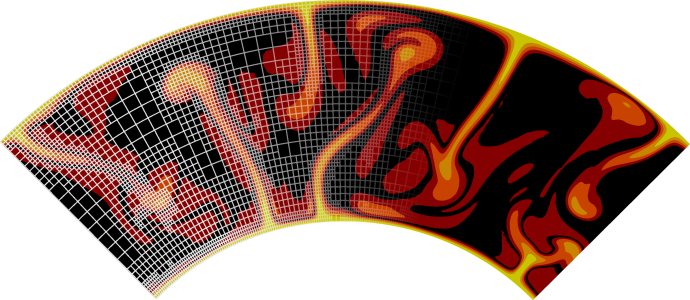
\includegraphics[height=1.25cm]{images/pictograms/aspect_logo}

\includegraphics[height=1.25cm]{images/pictograms/benchmark}

\includegraphics[height=1.25cm]{images/pictograms/triangle}

\includegraphics[height=1.25cm]{images/pictograms/FEM}

\includegraphics[height=1.25cm]{images/pictograms/paraview}

\includegraphics[height=1.25cm]{images/pictograms/publication}

%%%%%%%%%%%%%%%%%%%%%%%%%%%%%%%%%%%%%%%%%%%%%%%%%%%%%%%%%%%%%%%%%%%%%%%%%%%%%%%%%%%%%%%%%%%%%%%%%%%

\begin{flushright} {\tiny {\color{gray} python\_codes/fieldstone\_120/text.tex}} \end{flushright}

%\lstinputlisting[language=bash,basicstyle=\small]{python_codes/template_keywords.key}

\par\noindent\rule{\textwidth}{0.4pt}

\begin{center}
\inpython
{\small Code: \url{https://github.com/cedrict/fieldstone/tree/master/python_codes/fieldstone_120}}
\end{center}

\par\noindent\rule{\textwidth}{0.4pt}

%%%%%%%%%%%%%%%%%%%%%%%%%%%%%%%%%%%%%%%%%%%%%%%%%%%%%%%%%%%%%%%%%%%%%%%%%%%%%%%%%%%%%%%%%%%%%%%%%%%%

\index{stopics}{Donea \& Huerta mms}

This \stone was used to produce all the results in \textcite{thba24} (Subm.).

%======================
\section*{Philosophy}

The rationale behind this stone is as follows:
\begin{itemize}
\item create a library of basis functions and quadrature rules, as well as 
other FE-related tools so as to be able to write much more compact FE codes. 
So far the boundary conditions of this exercise are:
\begin{itemize}
\item Two-dimensional Cartesian domain
\item Continuous Galerkin method
\item Incompressible isothermal Stokes flow, but not isoviscous
\item Most of commonly used element pairs for Stokes equations + some more 'exotic' ones 
\item Dirichlet boundary conditions 
\item Isoparametric mapping 
\item Interior nodes positions with added randomness (if desired)
\item Stokes matrix fully built and sequential direct solver is used (REVISIT)
\item No stabilised formulations, i.e. no ${\bm Q}_1\times Q_1$-stab, 
      ${\bm Q}_1\times P_0$-stab, or $P_1\times P_1$-stab
\item No $P_1isoP_2$ or similar spaces
\item all triangles and quadrilaterals have straight edges.
\end{itemize}
\item Run a suite of manufactured solution benchmarks with all 
these finite element pairs and assess their accuracy.
\item show $L_2$ errors ($v$, $p$, div$(\vec\upnu)$) as function of $h$ and the 
total number of dofs (as in \textcite{cakp15} (2015))
\end{itemize}

\begin{remark}
{\bf 1)} For reasons explained in \textcite{bocg12} (2012) I use 
a symmetric grid ('SYMM') for triangular elements\footnote{See also remark 
of section 20.4.1 in \textcite{tesk12} (2012)} :
\begin{center} 
\includegraphics[width=10cm]{python_codes/fieldstone_120/images/bocg12}\\
{\captionfont Taken from \textcite{bocg12} (2012).}
\end{center} 
\end{remark}

\begin{remark}
{\bf 2)}Unless specified I set nelx=nely, i.e. the number of (quadrilateral) elements
in the $x$ and $y$ directions are equal.
\end{remark}

%%%%%%%%%%%%%%%%%%%%%%%%%%%%%%%%%%%%%%%%%%%%%%%%%%%%%%%%%%%%%%%%%%%%%%%%%%%%%%%
\section*{Finite element pairs for the Stokes equation}

\begin{center}
\begin{tabular}{p{1cm}p{2.75cm}p{3.5cm}p{2.25cm}p{6cm}}
\hline
 &pair & other name & information & remark \\
\hline
\hline
 1&${\bm Q}_1\times Q_0$       & ${\bm Q}_1\times P_0$       & Section~\ref{MMM-ss:pairq1p0} & NOT LBB STABLE but usable\\
 2&${\bm Q}_2\times Q_0$       &                             & Section~\ref{MMM-ss:pairq2q0}\\
 3&${\bm P}_2\times P_0$       &                             & Section~\ref{MMM-ss:p2p0}\\ 
 4&${\bm Q}_2\times Q_1$       &                             & Section~\ref{MMM-ss:pairq2q1}\\
 5&${\bm P}_2\times P_1$       &                             & Section~\ref{MMM-ss:p2p1}\\
 6&${\bm Q}_3\times Q_2$       &                             & Section~\ref{MMM-ss:q32d}\\
 7&${\bm P}_3\times P_2$       &                             & Section~\ref{MMM-ss:p3p2}\\
 8&${\bm Q}_1^+\times Q_1$     & Quad. MINI                  & Section~\ref{MMM-ss:quadmini}\\
 9&${\bm P}_1^+\times P_1$     & MINI                        & Section~\ref{MMM-pair:mini}\\
10&$RT_1\times Q_0$            &                             & Section~\ref{MMM-ss:RTq1p0}\\
11&$RT_2\times Q_0$            &                             & Section~\ref{MMM-ss:RTq1p0}\\
12&$DSSY_1\times Q_0$          &                             & Section~\ref{MMM-ss:pair_dssy2D}\\
13&$DSSY_2\times Q_0$          &                             & Section~\ref{MMM-ss:pair_dssy2D}\\
14&$Han\times Q_0$             &                             & Section~\ref{MMM-ss:han}\\
15&${\bm Q}_2\times P_{-1}$    &                             & Section~\ref{MMM-ss:pairq2pm1}\\
16&${\bm Q}_2\times P_{-1}(u)$ &                             & Section~\ref{MMM-ss:pairq2pm1}\\
17&${\bm Q}_2^{(8)}\times Q_1$ & Serendipity                 & Section~\ref{MMM-sec:serendipity2D}\\
18&${\bm P}_2^+\times P_{-1}$  & Crouzeix-Raviart            & Section~\ref{MMM-sec:crouzeix-raviart}\\
19&${\bm P}_2^+\times P_{1}$   &                             & Section~\ref{MMM-ss:p2pp1}\\
20&${\bm P}_2\times (P_1+P_0)$ & Augm. $P_2\times P_1$       & Section~\ref{MMM-ss:p2p1p0}\\
21&${\bm P}_1^{NC}\times P_0$  & Crouzeix-Raviart            & Section~\ref{MMM-ss:p1ncp0}\\
22&${\bm P}_1\times P_0$       &                             & Section~\ref{MMM-ss:p1p0}  &NOT LBB STABLE and unusable\\
23&${\bm Q}_2\times Q_{-1}$    &                             & Section~\ref{MMM-ss:pair_q2qm1} & NOT LBB STABLE\\
24&${\bm Q}_2\times Q_1+Q_0$   & Augm. ${\bm Q}_2\times Q_1$ & Section~\ref{MMM-ss:q2q1q0} \\
25&$Chen\times Q_0$            &                             & Section~\ref{MMM-ss:chenq0} & NOT SURE \\
26&${\bm Q}_4\times Q_3$       &                             & Section~\ref{MMM-ss:q42d}\\
27&${\bm P}_4\times P_3$       &                             & Section~\ref{MMM-ss:p4p3}\\
\hline
\end{tabular}
\end{center}

\begin{remark}
{\bf 3)} I have indeed built support for 3 unstable elements but 
these should not be included in the publication. 
\end{remark}

\begin{remark}
{\bf 4)} The augmented ${\bm P}_2\times (P_1+P_0)$ element pair is LBB stable 
but special care must be taken with respect to the rank-deficiency 
as explained in \textcite{bocg12} (2012). The same applies to ${\bm Q}_2\times (Q_1+Q_0)$. 
I propose a simple fix later. 
\end{remark}

\begin{remark}
{\bf 5)} The nonconforming ${\bm P}_1^{NC}\times P_0$ gives me a headache and does not 
yield accurate results (esp. the pressure). Not sure why... Coercivity/Korn stuff? I
have yet to find an article using the element 'as is'.
\end{remark}

\begin{remark}
{\bf 6)} Following \textcite{john16} book, I could also do 
${\bm P}_3^+\times P_{-2}$, ${\bm Q}_3\times P_{-2}$. 
\end{remark}

\begin{remark}
{\bf 7)} A modified $Q_2$ Serendipity element was proposed by \textcite{zhxi20} (2020) 
(see Section~\ref{MMM-sec:serendipity2Db}) but it is only different from the standard serendipity 
element when the elements are not rectangles. 
\end{remark}

\begin{remark}
{\bf 8)} Using high-order element spaces ($Q_4$, $P_4$, ...) only makes 
sense in this context if the manufactured solution is also a high-order polynomial 
or contains non-polynomial terms.
\end{remark}


\newpage
%%%%%%%%%%%%%%%%%%%%%%%%%%%%%%%%%%%%%%%%
\section*{velocity-pressure pair spaces}

\begin{center}
Quadrilateral elements\\
\begin{tabular}{ccccccc}
\hline
Vspace $\rightarrow$ & ${\bm Q}_1$  & ${\bm Q}_2$ & ${\bm Q}_2^{(8)}$ & ${\bm Q}_3$  & ${\bm Q}_4$ & ${\bm Q}_1^+$ \\ 
Pspace $\downarrow$ & \\
$Q_0$       & $\sqrt{}$ & $\sqrt{}$ & ?           & ?         &   & ?          \\
$Q_1$       & $\times$  & $\sqrt{}$ & $\sqrt{}$   & ?         &   & $\sqrt{}$  \\
$Q_2$       & $\times$  & $\times$  & $\times$    & $\sqrt{}$ &   & $\times$   \\
$Q_3$       & $\times$  & $\times$  & $\times$    & $\times$  & $\sqrt{}$ & $\times$ \\
$P_{-1}$    & ?         & $\sqrt{}$ & ?           & ?         &   & ?          \\
$P_{-1}(u)$ & ?         & $\sqrt{}$ & ?           & ?         &   & ?          \\
\hline
\end{tabular}
\end{center}

\begin{center}
Triangular elements\\
\begin{tabular}{cccccccc}
\hline
Vspace $\rightarrow$& ${\bm P}_1$ & ${\bm P}_2$ & ${\bm P}_3$ & ${\bm P}_4$ & ${\bm P}_1^+$ & ${\bm P}_2^+$ & ${\bm P}_1^{NC}$  \\
Pspace $\downarrow$ & \\
$P_0$    & $\times$ & $\sqrt{}$ & ?         & $\times$ &  ?        &  ?        & $\sqrt{}$   \\
$P_1$    & $\times$ & $\sqrt{}$ & ?         & $\times$ & $\sqrt{}$ &  ?        & ?           \\
$P_2$    & $\times$ & $\times$  & $\sqrt{}$ & $\times$ & $\times$  & $\times$  & $\times$    \\
$P_3$    & $\times$ & $\times$  & $\times$  & TODO     &           &           &             \\ 
$P_{-1}$ & $\times$ & $\sqrt{}$ & ?         &          &  ?        & $\sqrt{}$ & ?           \\
\hline
\end{tabular}
\end{center}


\newpage
%%%%%%%%%%%%%%%%%%%%%%%%%%%%%%%%%%%%%%%%
\section*{An attempt at classification}

\input{python_codes/fieldstone_120/tikz_potatoes}

$P_1^{nc} \times P_0$ belongs to non-conforming but it does not work.

\newpage
%%%%%%%%%%%%%%%%%%%%%%%%%%%%%%%%%%%%%%%%%%%%%%%%%%%%%%%%%%%%%%%%%%%%%%%%%%%%%%%
%%%%%%%%%%%%%%%%%%%%%%%%%%%%%%%%%%%%%%%%%%%%%%%%%%%%%%%%%%%%%%%%%%%%%%%%%%%%%%%
\section*{The libraries}

There are three files which contain all the required tools to build most of a FE code:

\begin{itemize}

\item {\pythonfile FEbasis2D.py} contains 

\begin{itemize}
\item \lstinline{NNN(r,s,space)}: returns the basis functions $\bN_i (i=1,...m)$ at position $r,s$.
\item \lstinline{dNNNdr(r,s,space)}: returns basis function derivative $\partial_r\bN_i (i=1,...m)$ at position $r,s$.
\item \lstinline{dNNNds(r,s,space)}: returns basis function derivative $\partial_s\bN_i (i=1,...m)$ at position $r,s$.
\item \lstinline{NNN_r(space)}: returns the $r_i (i=1,...m)$ coordinates of the support nodes.
\item \lstinline{NNN_s(space)}: returns the $s_i (i=1,...m)$ coordinates of the support nodes.

\item \lstinline{NNN_m(space)}: returns the number of support nodes.
\begin{lstlisting}
if space=='Q0':     return 1
if space=='P0':     return 1
if space=='Q1':     return 4
if space=='Q-1':    return 4
if space=='Q1+':    return 5
if space=='P1':     return 3
if space=='P1NC':   return 3
if space=='P-1':    return 3
if space=='Pm1':    return 3
if space=='Pm1u':   return 3
if space=='P1+':    return 4
if space=='P1+P0':  return 4
if space=='Q1+Q0':  return 5
if space=='Q2':     return 9
if space=='Q2s':    return 8
if space=='P2':     return 6
if space=='P2+':    return 7
if space=='P3':     return 10
if space=='P4':     return 15
if space=='Q3':     return 16
if space=='Q4':     return 25
if space=='DSSY1':  return 4
if space=='DSSY2':  return 4
if space=='RT1':    return 4
if space=='RT2':    return 4
if space=='Han':    return 5
if space=='Chen':   return 5
\end{lstlisting}


\item \lstinline{mapping(space)}: returns the type of mapping, i.e. $Q_1$ or $P_1$.
\item \lstinline{visualise_nodes(space)}: generates a pdf file with the support nodes 
and the shape of the reference element.
\item \lstinline{visualise_basis_functions(space)}: is an attempt at making a colormap of the basis functions.
\end{itemize}


\item {\pythonfile FEquadrature.py} contains
\begin{itemize}
\item \lstinline{quadrature(space,nqpts)}: it returns the number of quadrature points in the element, 
their coordinates and associated weights. If the element is a quadrilateral then it contains 
\lstinline{nqpts}$\times$\lstinline{nqpts} quadrature points. 
If it is a triangle then it contains \lstinline{nqpts} quadrature points in total. 
In that case only 3,6,7,12,13,16 are authorized.   
\item \lstinline{qcoords_1D(nqpts)}: returns the coordinates of the \lstinline{nqpts} quadrature points between -1 and 1.
Only used for quadrilateral elements.
\item \lstinline{qweights_1D(nqpts)}:returns the weights of the \lstinline{nqpts} quadrature points.
Only used for quadrilateral elements.
\item \lstinline{visualise_quadrature_points(space,nqpts)}: generates a pdf file.
\end{itemize}


\item {\pythonfile FEtools.py} contains

\begin{itemize}
\item \lstinline{cartesian_mesh(Lx,Ly,nelx,nely,space)}: Creates a cartesian mesh of \lstinline{nelx}
$\times$\lstinline{nely} elements in the domain $[0,L_x]\times[0,L_y]$. It returns the total 
number of nodes \lstinline{N}, the number of elements \lstinline{nel}, the coordinates of all the 
nodes in \lstinline{x,y} arrays and the connectivity array \lstinline{icon}.
There is an internal parameter \lstinline{mtype} which splits elements in 2 triangles 
if equal to zero, in 4 triangles if equal to 2, in 6 triangles in equal to 3.\\
\lstinline|mtype=0| can be used in combination with  $P_0$, $P_1$, $P_{-1}$, $P_1^+$, $P_1+P_0$ or $P_2$.\\
\lstinline|mtype=2| can be used in combination with  $P_0$, $P_1$.\\ 
\lstinline|mtype=3| can be used in combination with  $P_1$. 


\item \lstinline{randomize_background_mesh(x1,y1,hx,hy,N1,Lx,Ly)}: this adds a random perturbation
to the coordinates of all the nodes of the background mesh inside the domain (i.e. not on the boundary!). 
The amplitude of the perturbation is bounded by $0.1h_x$ and $0.1h_y$ in the $x$ and $y$ direction.

\item \lstinline{adapt_FE_mesh(x1,y1,icon1,m1,space1,x,y,icon,nel,space)}: This makes sure that 
all the support nodes for a given space are displaced so as to follow the randomized 
background mesh, using a (bi-)linear mapping.

\item \lstinline{export_swarm_to_ascii(x,y,filename)}:
\item \lstinline{export_swarm_scalar_to_ascii(x,y,f,filename)}:
\item \lstinline{export_swarm_vector_to_ascii(x,y,u,v,filename)}:
\item \lstinline{export_connectivity_array_to_ascii(x,y,icon,filename)}:
\item \lstinline{export_elements_to_vtu(x,y,icon,space,filename)}:
\item \lstinline{export_swarm_to_vtu(x,y,filename)}:
\item \lstinline{export_swarm_vector_to_vtu(x,y,vx,vy,filename)}:
\item \lstinline{export_swarm_scalar_to_vtu(x,y,scalar,filename)}:
\item \lstinline{bc_setup(x,y,Lx,Ly,ndof,left,right,bottom,top)}:
\item \lstinline{J(m,dNdr,dNds,x,y)}: computes the Jacobian matrix and its determinant 
for the mapping. 
\item \lstinline{assemble_K(K_el,A_sparse,iconV,mV,ndofV,iel)}:
\item \lstinline{assemble_G(G_el,A_sparse,iconV,iconP,NfemV,mV,mP,ndofV,ndofP,iel)}:
\item \lstinline{assemble_f(f_el,rhs,iconV,mV,ndofV,iel)}:
\item \lstinline{apply_bc(K_el,G_el,f_el,h_el,bc_val,bc_fix,iconV,mV,ndofV,iel)}:
\item \lstinline{visualise_with_tikz(x,y,space)}: generates a .tex file containing 
a tikz drawing of the nodes layout. Only works for $3\times 2$ meshes. 
\end{itemize}

\end{itemize}

\newpage
%%%%%%%%%%%%%%%%%%%%%%%%%%%%%%%%%%%%%%%%%%%%%%%%%%%%%%%%%%%%%%%%%%%%%%%%%%%%%%%
%%%%%%%%%%%%%%%%%%%%%%%%%%%%%%%%%%%%%%%%%%%%%%%%%%%%%%%%%%%%%%%%%%%%%%%%%%%%%%%
\section*{tester \#1}

{\pythonfile tester1.py}: checks that each basis function is 1 on its support node and zero at all other nodes.



\begin{scriptsize}
\begin{verbatim}
=========================================
 tester 1: nodes
=========================================
=========================================
 Q0
=========================================
m= 1
node 0 : [1.]
=========================================
 Q1
=========================================
m= 4
node 0 : [1. 0. 0. 0.]
node 1 : [0. 1. 0. 0.]
node 2 : [0. 0. 1. 0.]
node 3 : [0. 0. 0. 1.]
=========================================
 Q1+
=========================================
m= 5
node 0 : [1. 0. 0. 0. 0.]
node 1 : [0. 1. 0. 0. 0.]
node 2 : [0. 0. 1. 0. 0.]
node 3 : [0. 0. 0. 1. 0.]
node 4 : [0. 0. 0. 0. 1.]
=========================================
 Q2
=========================================
m= 9
node 0 : [ 1. -0.  0. -0.  0. -0. -0.  0.  0.]
node 1 : [ 0.  1. -0. -0.  0.  0. -0.  0.  0.]
node 2 : [0. 0. 1. 0. 0. 0. 0. 0. 0.]
node 3 : [ 0. -0. -0.  1.  0. -0.  0.  0.  0.]
node 4 : [-0.  0. -0.  0.  1.  0. -0. -0.  0.]
node 5 : [-0. -0.  0.  0. -0.  1.  0.  0.  0.]
node 6 : [-0.  0.  0. -0.  0.  0.  1. -0.  0.]
node 7 : [-0.  0. -0.  0. -0. -0.  0.  1.  0.]
node 8 : [ 0. -0.  0. -0. -0.  0.  0. -0.  1.]
=========================================
 Q3
=========================================
m= 16
node 0 : [1. 0. 0. 0. 0. 0. 0. 0. 0. 0. 0. 0. 0. 0. 0. 0.]
node 1 : [ 0.00000000e+00  1.00000000e+00 -1.38777878e-17  0.00000000e+00
  0.00000000e+00  0.00000000e+00 -0.00000000e+00  0.00000000e+00
  0.00000000e+00  0.00000000e+00 -0.00000000e+00  0.00000000e+00
  0.00000000e+00  0.00000000e+00 -0.00000000e+00  0.00000000e+00]
node 2 : [ 0.00000000e+00 -1.38777878e-17  1.00000000e+00  0.00000000e+00
  0.00000000e+00 -0.00000000e+00  0.00000000e+00  0.00000000e+00
  0.00000000e+00 -0.00000000e+00  0.00000000e+00  0.00000000e+00
  0.00000000e+00 -0.00000000e+00  0.00000000e+00  0.00000000e+00]
node 3 : [0. 0. 0. 1. 0. 0. 0. 0. 0. 0. 0. 0. 0. 0. 0. 0.]
node 4 : [ 0.00000000e+00  0.00000000e+00  0.00000000e+00  0.00000000e+00
  1.00000000e+00  0.00000000e+00  0.00000000e+00  0.00000000e+00
 -1.38777878e-17 -0.00000000e+00 -0.00000000e+00 -0.00000000e+00
  0.00000000e+00  0.00000000e+00  0.00000000e+00  0.00000000e+00]
node 5 : [ 0.00000000e+00  0.00000000e+00 -0.00000000e+00  0.00000000e+00
  0.00000000e+00  1.00000000e+00 -1.38777878e-17  0.00000000e+00
 -0.00000000e+00 -1.38777878e-17  1.92592994e-34 -0.00000000e+00
  0.00000000e+00  0.00000000e+00 -0.00000000e+00  0.00000000e+00]
node 6 : [ 0.00000000e+00 -0.00000000e+00  0.00000000e+00  0.00000000e+00
  0.00000000e+00 -1.38777878e-17  1.00000000e+00  0.00000000e+00
 -0.00000000e+00  1.92592994e-34 -1.38777878e-17 -0.00000000e+00
  0.00000000e+00 -0.00000000e+00  0.00000000e+00  0.00000000e+00]
node 7 : [ 0.00000000e+00  0.00000000e+00  0.00000000e+00  0.00000000e+00
  0.00000000e+00  0.00000000e+00  0.00000000e+00  1.00000000e+00
 -0.00000000e+00 -0.00000000e+00 -0.00000000e+00 -1.38777878e-17
  0.00000000e+00  0.00000000e+00  0.00000000e+00  0.00000000e+00]
node 8 : [ 0.00000000e+00  0.00000000e+00  0.00000000e+00  0.00000000e+00
 -1.38777878e-17 -0.00000000e+00 -0.00000000e+00 -0.00000000e+00
  1.00000000e+00  0.00000000e+00  0.00000000e+00  0.00000000e+00
  0.00000000e+00  0.00000000e+00  0.00000000e+00  0.00000000e+00]
node 9 : [ 0.00000000e+00  0.00000000e+00 -0.00000000e+00  0.00000000e+00
 -0.00000000e+00 -1.38777878e-17  1.92592994e-34 -0.00000000e+00
  0.00000000e+00  1.00000000e+00 -1.38777878e-17  0.00000000e+00
  0.00000000e+00  0.00000000e+00 -0.00000000e+00  0.00000000e+00]
node 10 : [ 0.00000000e+00 -0.00000000e+00  0.00000000e+00  0.00000000e+00
 -0.00000000e+00  1.92592994e-34 -1.38777878e-17 -0.00000000e+00
  0.00000000e+00 -1.38777878e-17  1.00000000e+00  0.00000000e+00
  0.00000000e+00 -0.00000000e+00  0.00000000e+00  0.00000000e+00]
node 11 : [ 0.00000000e+00  0.00000000e+00  0.00000000e+00  0.00000000e+00
 -0.00000000e+00 -0.00000000e+00 -0.00000000e+00 -1.38777878e-17
  0.00000000e+00  0.00000000e+00  0.00000000e+00  1.00000000e+00
  0.00000000e+00  0.00000000e+00  0.00000000e+00  0.00000000e+00]
node 12 : [0. 0. 0. 0. 0. 0. 0. 0. 0. 0. 0. 0. 1. 0. 0. 0.]
node 13 : [ 0.00000000e+00  0.00000000e+00 -0.00000000e+00  0.00000000e+00
  0.00000000e+00  0.00000000e+00 -0.00000000e+00  0.00000000e+00
  0.00000000e+00  0.00000000e+00 -0.00000000e+00  0.00000000e+00
  0.00000000e+00  1.00000000e+00 -1.38777878e-17  0.00000000e+00]
node 14 : [ 0.00000000e+00 -0.00000000e+00  0.00000000e+00  0.00000000e+00
  0.00000000e+00 -0.00000000e+00  0.00000000e+00  0.00000000e+00
  0.00000000e+00 -0.00000000e+00  0.00000000e+00  0.00000000e+00
  0.00000000e+00 -1.38777878e-17  1.00000000e+00  0.00000000e+00]
node 15 : [0. 0. 0. 0. 0. 0. 0. 0. 0. 0. 0. 0. 0. 0. 0. 1.]
=========================================
 Q2s
=========================================
m= 8
node 0 : [ 1. -0. -0. -0.  0.  0.  0.  0.]
node 1 : [-0.  1. -0. -0.  0.  0.  0.  0.]
node 2 : [-0. -0.  1. -0.  0.  0.  0.  0.]
node 3 : [-0. -0. -0.  1.  0.  0.  0.  0.]
node 4 : [ 0.  0. -0. -0.  1.  0.  0.  0.]
node 5 : [-0.  0.  0. -0.  0.  1.  0.  0.]
node 6 : [-0. -0.  0.  0.  0.  0.  1.  0.]
node 7 : [ 0. -0. -0.  0.  0.  0.  0.  1.]
=========================================
 P0
=========================================
m= 1
node 0 : [1.]
=========================================
 P1
=========================================
m= 3
node 0 : [1. 0. 0.]
node 1 : [0. 1. 0.]
node 2 : [0. 0. 1.]
=========================================
 P1+
=========================================
m= 4
node 0 : [1. 0. 0. 0.]
node 1 : [0. 1. 0. 0.]
node 2 : [0. 0. 1. 0.]
node 3 : [ 5.55111512e-17 -5.55111512e-17 -5.55111512e-17  1.00000000e+00]
=========================================
 P1NC
=========================================
m= 3
node 0 : [1. 0. 0.]
node 1 : [0. 1. 0.]
node 2 : [0. 0. 1.]
=========================================
 P2
=========================================
m= 6
node 0 : [1. 0. 0. 0. 0. 0.]
node 1 : [0. 1. 0. 0. 0. 0.]
node 2 : [0. 0. 1. 0. 0. 0.]
node 3 : [0. 0. 0. 1. 0. 0.]
node 4 : [0. 0. 0. 0. 1. 0.]
node 5 : [0. 0. 0. 0. 0. 1.]
=========================================
 P3
=========================================
m= 10
node 0 : [1. 0. 0. 0. 0. 0. 0. 0. 0. 0.]
node 1 : [ 1.11022302e-16  1.00000000e+00  1.11022302e-16 -5.55111512e-17
  0.00000000e+00  0.00000000e+00  0.00000000e+00  0.00000000e+00
  0.00000000e+00  0.00000000e+00]
node 2 : [ 4.4408921e-16 -8.8817842e-16  1.0000000e+00 -4.4408921e-16
  0.0000000e+00  0.0000000e+00  0.0000000e+00  0.0000000e+00
  0.0000000e+00  0.0000000e+00]
node 3 : [0. 0. 0. 1. 0. 0. 0. 0. 0. 0.]
node 4 : [ 1.11022302e-16  0.00000000e+00  0.00000000e+00  0.00000000e+00
  1.00000000e+00  0.00000000e+00  0.00000000e+00  1.11022302e-16
  0.00000000e+00 -5.55111512e-17]
node 5 : [ 3.33066907e-16  0.00000000e+00  1.11022302e-16 -5.55111512e-17
 -1.11022302e-16  1.00000000e+00  0.00000000e+00  1.11022302e-16
  0.00000000e+00 -5.55111512e-17]
node 6 : [ 3.33066907e-16 -8.88178420e-16  8.88178420e-16 -4.44089210e-16
 -1.11022302e-16  0.00000000e+00  1.00000000e+00  1.11022302e-16
  0.00000000e+00 -5.55111512e-17]
node 7 : [ 4.4408921e-16  0.0000000e+00  0.0000000e+00  0.0000000e+00
 -8.8817842e-16  0.0000000e+00  0.0000000e+00  1.0000000e+00
  0.0000000e+00 -4.4408921e-16]
node 8 : [ 0.00000000e+00  0.00000000e+00  0.00000000e+00 -5.55111512e-17
 -8.88178420e-16  0.00000000e+00  0.00000000e+00  8.88178420e-16
  1.00000000e+00 -4.44089210e-16]
node 9 : [0. 0. 0. 0. 0. 0. 0. 0. 0. 1.]
=========================================
 P4
=========================================
m= 15
node 0 : [1. 0. 0. 0. 0. 0. 0. 0. 0. 0. 0. 0. 0. 0. 0.]
node 1 : [0. 1. 0. 0. 0. 0. 0. 0. 0. 0. 0. 0. 0. 0. 0.]
node 2 : [0. 0. 1. 0. 0. 0. 0. 0. 0. 0. 0. 0. 0. 0. 0.]
node 3 : [0. 0. 0. 1. 0. 0. 0. 0. 0. 0. 0. 0. 0. 0. 0.]
node 4 : [0. 0. 0. 0. 1. 0. 0. 0. 0. 0. 0. 0. 0. 0. 0.]
node 5 : [0. 0. 0. 0. 0. 1. 0. 0. 0. 0. 0. 0. 0. 0. 0.]
node 6 : [0. 0. 0. 0. 0. 0. 1. 0. 0. 0. 0. 0. 0. 0. 0.]
node 7 : [0. 0. 0. 0. 0. 0. 0. 1. 0. 0. 0. 0. 0. 0. 0.]
node 8 : [0. 0. 0. 0. 0. 0. 0. 0. 1. 0. 0. 0. 0. 0. 0.]
node 9 : [0. 0. 0. 0. 0. 0. 0. 0. 0. 1. 0. 0. 0. 0. 0.]
node 10 : [0. 0. 0. 0. 0. 0. 0. 0. 0. 0. 1. 0. 0. 0. 0.]
node 11 : [0. 0. 0. 0. 0. 0. 0. 0. 0. 0. 0. 1. 0. 0. 0.]
node 12 : [0. 0. 0. 0. 0. 0. 0. 0. 0. 0. 0. 0. 1. 0. 0.]
node 13 : [0. 0. 0. 0. 0. 0. 0. 0. 0. 0. 0. 0. 0. 1. 0.]
node 14 : [0. 0. 0. 0. 0. 0. 0. 0. 0. 0. 0. 0. 0. 0. 1.]
=========================================
 P1+P0
=========================================
m= 4
node 0 : [1. 0. 0. 1.]
node 1 : [0. 1. 0. 1.]
node 2 : [0. 0. 1. 1.]
node 3 : [0.33333333 0.33333333 0.33333333 1.        ]
=========================================
 DSSY1
=========================================
m= 4
node 0 : [1. 0. 0. 0.]
node 1 : [0. 1. 0. 0.]
node 2 : [0. 0. 1. 0.]
node 3 : [0. 0. 0. 1.]
=========================================
 DSSY2
=========================================
m= 4
node 0 : [1. 0. 0. 0.]
node 1 : [0. 1. 0. 0.]
node 2 : [0. 0. 1. 0.]
node 3 : [0. 0. 0. 1.]
=========================================
 RT1
=========================================
m= 4
node 0 : [1. 0. 0. 0.]
node 1 : [0. 1. 0. 0.]
node 2 : [0. 0. 1. 0.]
node 3 : [0. 0. 0. 1.]
=========================================
 RT2
=========================================
m= 4
node 0 : [ 1.125 -0.125  0.125 -0.125]
node 1 : [-0.125  1.125 -0.125  0.125]
node 2 : [ 0.125 -0.125  1.125 -0.125]
node 3 : [-0.125  0.125 -0.125  1.125]
=========================================
 Han
=========================================
m= 5
node 0 : [ 1.  0.  0. -0.  0.]
node 1 : [-0.  1.  0. -0.  0.]
node 2 : [-0.  0.  1. -0.  0.]
node 3 : [-0.  0.  0.  1.  0.]
node 4 : [-0.  0.  0. -0.  1.]
=========================================
 Chen
=========================================
m= 5
node 0 : [1.   0.   0.   0.   0.25]
node 1 : [0.   1.   0.   0.   0.25]
node 2 : [0.   0.   1.   0.   0.25]
node 3 : [0.   0.   0.   1.   0.25]
node 4 : [0.25 0.25 0.25 0.25 1.  ]

\end{verbatim}
\end{scriptsize}


\newpage
%%%%%%%%%%%%%%%%%%%%%%%%%%%%%%%%%%%%%%%%%%%%%%%%%%%%%%%%%%%%%%%%%%%%%%%%%%%%%%%
%%%%%%%%%%%%%%%%%%%%%%%%%%%%%%%%%%%%%%%%%%%%%%%%%%%%%%%%%%%%%%%%%%%%%%%%%%%%%%%
\section*{tester \#2}

{\pythonfile tester2.py}: computes the area of each element by means of numerical 
quadrature. The domain is $3 \times 2$ and there are $3 \times 2$ elements so that we expect 1 for 
quadrilateral elements and 0.5 for triangular elements.  

\begin{tiny}
\begin{verbatim}

=========================================
 tester 2: areas
=========================================
=========================================
 Q1
=========================================
nqel= 9
iel= 0 | iq= 0 | jcob= 2.00 0.00 0.00 2.00 0.25
iel= 0 | iq= 1 | jcob= 2.00 0.00 0.00 2.00 0.25
iel= 0 | iq= 2 | jcob= 2.00 0.00 0.00 2.00 0.25
iel= 0 | iq= 3 | jcob= 2.00 0.00 0.00 2.00 0.25
iel= 0 | iq= 4 | jcob= 2.00 0.00 0.00 2.00 0.25
iel= 0 | iq= 5 | jcob= 2.00 0.00 0.00 2.00 0.25
iel= 0 | iq= 6 | jcob= 2.00 0.00 0.00 2.00 0.25
iel= 0 | iq= 7 | jcob= 2.00 0.00 0.00 2.00 0.25
iel= 0 | iq= 8 | jcob= 2.00 0.00 0.00 2.00 0.25
iel= 1 | iq= 0 | jcob= 2.00 0.00 0.00 2.00 0.25
iel= 1 | iq= 1 | jcob= 2.00 0.00 0.00 2.00 0.25
iel= 1 | iq= 2 | jcob= 2.00 0.00 0.00 2.00 0.25
iel= 1 | iq= 3 | jcob= 2.00 0.00 0.00 2.00 0.25
iel= 1 | iq= 4 | jcob= 2.00 0.00 0.00 2.00 0.25
iel= 1 | iq= 5 | jcob= 2.00 0.00 0.00 2.00 0.25
iel= 1 | iq= 6 | jcob= 2.00 0.00 0.00 2.00 0.25
iel= 1 | iq= 7 | jcob= 2.00 0.00 0.00 2.00 0.25
iel= 1 | iq= 8 | jcob= 2.00 0.00 0.00 2.00 0.25
iel= 2 | iq= 0 | jcob= 2.00 0.00 0.00 2.00 0.25
iel= 2 | iq= 1 | jcob= 2.00 0.00 0.00 2.00 0.25
iel= 2 | iq= 2 | jcob= 2.00 0.00 0.00 2.00 0.25
iel= 2 | iq= 3 | jcob= 2.00 0.00 0.00 2.00 0.25
iel= 2 | iq= 4 | jcob= 2.00 0.00 0.00 2.00 0.25
iel= 2 | iq= 5 | jcob= 2.00 0.00 0.00 2.00 0.25
iel= 2 | iq= 6 | jcob= 2.00 0.00 0.00 2.00 0.25
iel= 2 | iq= 7 | jcob= 2.00 0.00 0.00 2.00 0.25
iel= 2 | iq= 8 | jcob= 2.00 0.00 0.00 2.00 0.25
iel= 3 | iq= 0 | jcob= 2.00 0.00 0.00 2.00 0.25
iel= 3 | iq= 1 | jcob= 2.00 0.00 0.00 2.00 0.25
iel= 3 | iq= 2 | jcob= 2.00 0.00 0.00 2.00 0.25
iel= 3 | iq= 3 | jcob= 2.00 0.00 0.00 2.00 0.25
iel= 3 | iq= 4 | jcob= 2.00 0.00 0.00 2.00 0.25
iel= 3 | iq= 5 | jcob= 2.00 0.00 0.00 2.00 0.25
iel= 3 | iq= 6 | jcob= 2.00 0.00 0.00 2.00 0.25
iel= 3 | iq= 7 | jcob= 2.00 0.00 0.00 2.00 0.25
iel= 3 | iq= 8 | jcob= 2.00 0.00 0.00 2.00 0.25
iel= 4 | iq= 0 | jcob= 2.00 0.00 0.00 2.00 0.25
iel= 4 | iq= 1 | jcob= 2.00 0.00 0.00 2.00 0.25
iel= 4 | iq= 2 | jcob= 2.00 0.00 0.00 2.00 0.25
iel= 4 | iq= 3 | jcob= 2.00 0.00 0.00 2.00 0.25
iel= 4 | iq= 4 | jcob= 2.00 0.00 0.00 2.00 0.25
iel= 4 | iq= 5 | jcob= 2.00 0.00 0.00 2.00 0.25
iel= 4 | iq= 6 | jcob= 2.00 0.00 0.00 2.00 0.25
iel= 4 | iq= 7 | jcob= 2.00 0.00 0.00 2.00 0.25
iel= 4 | iq= 8 | jcob= 2.00 0.00 0.00 2.00 0.25
iel= 5 | iq= 0 | jcob= 2.00 0.00 0.00 2.00 0.25
iel= 5 | iq= 1 | jcob= 2.00 0.00 0.00 2.00 0.25
iel= 5 | iq= 2 | jcob= 2.00 0.00 0.00 2.00 0.25
iel= 5 | iq= 3 | jcob= 2.00 0.00 0.00 2.00 0.25
iel= 5 | iq= 4 | jcob= 2.00 0.00 0.00 2.00 0.25
iel= 5 | iq= 5 | jcob= 2.00 0.00 0.00 2.00 0.25
iel= 5 | iq= 6 | jcob= 2.00 0.00 0.00 2.00 0.25
iel= 5 | iq= 7 | jcob= 2.00 0.00 0.00 2.00 0.25
iel= 5 | iq= 8 | jcob= 2.00 0.00 0.00 2.00 0.25
areas= [1. 1. 1. 1. 1. 1.]
=========================================
 Q1+
=========================================
nqel= 9
iel= 0 | iq= 0 | jcob= 2.00 0.00 0.00 2.00 0.25
iel= 0 | iq= 1 | jcob= 2.00 0.00 0.00 2.00 0.25
iel= 0 | iq= 2 | jcob= 2.00 0.00 0.00 2.00 0.25
iel= 0 | iq= 3 | jcob= 2.00 0.00 0.00 2.00 0.25
iel= 0 | iq= 4 | jcob= 2.00 0.00 0.00 2.00 0.25
iel= 0 | iq= 5 | jcob= 2.00 -0.00 0.00 2.00 0.25
iel= 0 | iq= 6 | jcob= 2.00 0.00 0.00 2.00 0.25
iel= 0 | iq= 7 | jcob= 2.00 0.00 -0.00 2.00 0.25
iel= 0 | iq= 8 | jcob= 2.00 -0.00 -0.00 2.00 0.25
iel= 1 | iq= 0 | jcob= 2.00 0.00 -0.00 2.00 0.25
iel= 1 | iq= 1 | jcob= 2.00 0.00 0.00 2.00 0.25
iel= 1 | iq= 2 | jcob= 2.00 0.00 0.00 2.00 0.25
iel= 1 | iq= 3 | jcob= 2.00 0.00 0.00 2.00 0.25
iel= 1 | iq= 4 | jcob= 2.00 0.00 0.00 2.00 0.25
iel= 1 | iq= 5 | jcob= 2.00 -0.00 0.00 2.00 0.25
iel= 1 | iq= 6 | jcob= 2.00 0.00 0.00 2.00 0.25
iel= 1 | iq= 7 | jcob= 2.00 0.00 -0.00 2.00 0.25
iel= 1 | iq= 8 | jcob= 2.00 -0.00 -0.00 2.00 0.25
iel= 2 | iq= 0 | jcob= 2.00 0.00 0.00 2.00 0.25
iel= 2 | iq= 1 | jcob= 2.00 0.00 0.00 2.00 0.25
iel= 2 | iq= 2 | jcob= 2.00 0.00 0.00 2.00 0.25
iel= 2 | iq= 3 | jcob= 2.00 0.00 0.00 2.00 0.25
iel= 2 | iq= 4 | jcob= 2.00 0.00 0.00 2.00 0.25
iel= 2 | iq= 5 | jcob= 2.00 -0.00 -0.00 2.00 0.25
iel= 2 | iq= 6 | jcob= 2.00 0.00 -0.00 2.00 0.25
iel= 2 | iq= 7 | jcob= 2.00 0.00 0.00 2.00 0.25
iel= 2 | iq= 8 | jcob= 2.00 -0.00 -0.00 2.00 0.25
iel= 3 | iq= 0 | jcob= 2.00 -0.00 0.00 2.00 0.25
iel= 3 | iq= 1 | jcob= 2.00 0.00 0.00 2.00 0.25
iel= 3 | iq= 2 | jcob= 2.00 0.00 0.00 2.00 0.25
iel= 3 | iq= 3 | jcob= 2.00 0.00 0.00 2.00 0.25
iel= 3 | iq= 4 | jcob= 2.00 0.00 0.00 2.00 0.25
iel= 3 | iq= 5 | jcob= 2.00 -0.00 0.00 2.00 0.25
iel= 3 | iq= 6 | jcob= 2.00 0.00 0.00 2.00 0.25
iel= 3 | iq= 7 | jcob= 2.00 0.00 -0.00 2.00 0.25
iel= 3 | iq= 8 | jcob= 2.00 -0.00 -0.00 2.00 0.25
iel= 4 | iq= 0 | jcob= 2.00 -0.00 -0.00 2.00 0.25
iel= 4 | iq= 1 | jcob= 2.00 0.00 0.00 2.00 0.25
iel= 4 | iq= 2 | jcob= 2.00 0.00 0.00 2.00 0.25
iel= 4 | iq= 3 | jcob= 2.00 0.00 0.00 2.00 0.25
iel= 4 | iq= 4 | jcob= 2.00 0.00 0.00 2.00 0.25
iel= 4 | iq= 5 | jcob= 2.00 -0.00 0.00 2.00 0.25
iel= 4 | iq= 6 | jcob= 2.00 0.00 0.00 2.00 0.25
iel= 4 | iq= 7 | jcob= 2.00 0.00 -0.00 2.00 0.25
iel= 4 | iq= 8 | jcob= 2.00 -0.00 -0.00 2.00 0.25
iel= 5 | iq= 0 | jcob= 2.00 -0.00 0.00 2.00 0.25
iel= 5 | iq= 1 | jcob= 2.00 0.00 0.00 2.00 0.25
iel= 5 | iq= 2 | jcob= 2.00 0.00 0.00 2.00 0.25
iel= 5 | iq= 3 | jcob= 2.00 0.00 0.00 2.00 0.25
iel= 5 | iq= 4 | jcob= 2.00 0.00 0.00 2.00 0.25
iel= 5 | iq= 5 | jcob= 2.00 -0.00 -0.00 2.00 0.25
iel= 5 | iq= 6 | jcob= 2.00 0.00 -0.00 2.00 0.25
iel= 5 | iq= 7 | jcob= 2.00 0.00 0.00 2.00 0.25
iel= 5 | iq= 8 | jcob= 2.00 -0.00 -0.00 2.00 0.25
areas= [1. 1. 1. 1. 1. 1.]
=========================================
 Q2
=========================================
nqel= 9
iel= 0 | iq= 0 | jcob= 2.00 0.00 0.00 2.00 0.25
iel= 0 | iq= 1 | jcob= 2.00 0.00 0.00 2.00 0.25
iel= 0 | iq= 2 | jcob= 2.00 -0.00 0.00 2.00 0.25
iel= 0 | iq= 3 | jcob= 2.00 0.00 0.00 2.00 0.25
iel= 0 | iq= 4 | jcob= 2.00 0.00 0.00 2.00 0.25
iel= 0 | iq= 5 | jcob= 2.00 0.00 0.00 2.00 0.25
iel= 0 | iq= 6 | jcob= 2.00 0.00 0.00 2.00 0.25
iel= 0 | iq= 7 | jcob= 2.00 0.00 0.00 2.00 0.25
iel= 0 | iq= 8 | jcob= 2.00 0.00 -0.00 2.00 0.25
iel= 1 | iq= 0 | jcob= 2.00 0.00 -0.00 2.00 0.25
iel= 1 | iq= 1 | jcob= 2.00 0.00 0.00 2.00 0.25
iel= 1 | iq= 2 | jcob= 2.00 -0.00 0.00 2.00 0.25
iel= 1 | iq= 3 | jcob= 2.00 0.00 0.00 2.00 0.25
iel= 1 | iq= 4 | jcob= 2.00 0.00 0.00 2.00 0.25
iel= 1 | iq= 5 | jcob= 2.00 0.00 0.00 2.00 0.25
iel= 1 | iq= 6 | jcob= 2.00 0.00 -0.00 2.00 0.25
iel= 1 | iq= 7 | jcob= 2.00 0.00 0.00 2.00 0.25
iel= 1 | iq= 8 | jcob= 2.00 0.00 0.00 2.00 0.25
iel= 2 | iq= 0 | jcob= 2.00 0.00 0.00 2.00 0.25
iel= 2 | iq= 1 | jcob= 2.00 0.00 0.00 2.00 0.25
iel= 2 | iq= 2 | jcob= 2.00 -0.00 0.00 2.00 0.25
iel= 2 | iq= 3 | jcob= 2.00 0.00 0.00 2.00 0.25
iel= 2 | iq= 4 | jcob= 2.00 0.00 0.00 2.00 0.25
iel= 2 | iq= 5 | jcob= 2.00 0.00 0.00 2.00 0.25
iel= 2 | iq= 6 | jcob= 2.00 0.00 -0.00 2.00 0.25
iel= 2 | iq= 7 | jcob= 2.00 0.00 0.00 2.00 0.25
iel= 2 | iq= 8 | jcob= 2.00 0.00 0.00 2.00 0.25
iel= 3 | iq= 0 | jcob= 2.00 -0.00 0.00 2.00 0.25
iel= 3 | iq= 1 | jcob= 2.00 0.00 0.00 2.00 0.25
iel= 3 | iq= 2 | jcob= 2.00 -0.00 0.00 2.00 0.25
iel= 3 | iq= 3 | jcob= 2.00 0.00 0.00 2.00 0.25
iel= 3 | iq= 4 | jcob= 2.00 0.00 0.00 2.00 0.25
iel= 3 | iq= 5 | jcob= 2.00 0.00 0.00 2.00 0.25
iel= 3 | iq= 6 | jcob= 2.00 0.00 0.00 2.00 0.25
iel= 3 | iq= 7 | jcob= 2.00 0.00 0.00 2.00 0.25
iel= 3 | iq= 8 | jcob= 2.00 0.00 -0.00 2.00 0.25
iel= 4 | iq= 0 | jcob= 2.00 -0.00 -0.00 2.00 0.25
iel= 4 | iq= 1 | jcob= 2.00 0.00 0.00 2.00 0.25
iel= 4 | iq= 2 | jcob= 2.00 -0.00 0.00 2.00 0.25
iel= 4 | iq= 3 | jcob= 2.00 0.00 0.00 2.00 0.25
iel= 4 | iq= 4 | jcob= 2.00 0.00 0.00 2.00 0.25
iel= 4 | iq= 5 | jcob= 2.00 0.00 0.00 2.00 0.25
iel= 4 | iq= 6 | jcob= 2.00 0.00 -0.00 2.00 0.25
iel= 4 | iq= 7 | jcob= 2.00 0.00 0.00 2.00 0.25
iel= 4 | iq= 8 | jcob= 2.00 0.00 0.00 2.00 0.25
iel= 5 | iq= 0 | jcob= 2.00 -0.00 0.00 2.00 0.25
iel= 5 | iq= 1 | jcob= 2.00 0.00 0.00 2.00 0.25
iel= 5 | iq= 2 | jcob= 2.00 -0.00 0.00 2.00 0.25
iel= 5 | iq= 3 | jcob= 2.00 0.00 0.00 2.00 0.25
iel= 5 | iq= 4 | jcob= 2.00 0.00 0.00 2.00 0.25
iel= 5 | iq= 5 | jcob= 2.00 0.00 0.00 2.00 0.25
iel= 5 | iq= 6 | jcob= 2.00 0.00 -0.00 2.00 0.25
iel= 5 | iq= 7 | jcob= 2.00 0.00 0.00 2.00 0.25
iel= 5 | iq= 8 | jcob= 2.00 0.00 0.00 2.00 0.25
areas= [1. 1. 1. 1. 1. 1.]
=========================================
 Q3
=========================================
nqel= 9
iel= 0 | iq= 0 | jcob= 2.00 -0.00 0.00 2.00 0.25
iel= 0 | iq= 1 | jcob= 2.00 0.00 0.00 2.00 0.25
iel= 0 | iq= 2 | jcob= 2.00 0.00 -0.00 2.00 0.25
iel= 0 | iq= 3 | jcob= 2.00 0.00 0.00 2.00 0.25
iel= 0 | iq= 4 | jcob= 2.00 0.00 0.00 2.00 0.25
iel= 0 | iq= 5 | jcob= 2.00 0.00 -0.00 2.00 0.25
iel= 0 | iq= 6 | jcob= 2.00 0.00 0.00 2.00 0.25
iel= 0 | iq= 7 | jcob= 2.00 -0.00 0.00 2.00 0.25
iel= 0 | iq= 8 | jcob= 2.00 0.00 -0.00 2.00 0.25
iel= 1 | iq= 0 | jcob= 2.00 -0.00 0.00 2.00 0.25
iel= 1 | iq= 1 | jcob= 2.00 0.00 0.00 2.00 0.25
iel= 1 | iq= 2 | jcob= 2.00 0.00 -0.00 2.00 0.25
iel= 1 | iq= 3 | jcob= 2.00 0.00 0.00 2.00 0.25
iel= 1 | iq= 4 | jcob= 2.00 0.00 0.00 2.00 0.25
iel= 1 | iq= 5 | jcob= 2.00 0.00 -0.00 2.00 0.25
iel= 1 | iq= 6 | jcob= 2.00 0.00 -0.00 2.00 0.25
iel= 1 | iq= 7 | jcob= 2.00 -0.00 0.00 2.00 0.25
iel= 1 | iq= 8 | jcob= 2.00 0.00 0.00 2.00 0.25
iel= 2 | iq= 0 | jcob= 2.00 -0.00 -0.00 2.00 0.25
iel= 2 | iq= 1 | jcob= 2.00 0.00 0.00 2.00 0.25
iel= 2 | iq= 2 | jcob= 2.00 0.00 0.00 2.00 0.25
iel= 2 | iq= 3 | jcob= 2.00 0.00 0.00 2.00 0.25
iel= 2 | iq= 4 | jcob= 2.00 0.00 0.00 2.00 0.25
iel= 2 | iq= 5 | jcob= 2.00 0.00 -0.00 2.00 0.25
iel= 2 | iq= 6 | jcob= 2.00 0.00 0.00 2.00 0.25
iel= 2 | iq= 7 | jcob= 2.00 -0.00 0.00 2.00 0.25
iel= 2 | iq= 8 | jcob= 2.00 0.00 -0.00 2.00 0.25
iel= 3 | iq= 0 | jcob= 2.00 -0.00 0.00 2.00 0.25
iel= 3 | iq= 1 | jcob= 2.00 0.00 0.00 2.00 0.25
iel= 3 | iq= 2 | jcob= 2.00 0.00 -0.00 2.00 0.25
iel= 3 | iq= 3 | jcob= 2.00 0.00 0.00 2.00 0.25
iel= 3 | iq= 4 | jcob= 2.00 0.00 0.00 2.00 0.25
iel= 3 | iq= 5 | jcob= 2.00 0.00 -0.00 2.00 0.25
iel= 3 | iq= 6 | jcob= 2.00 0.00 0.00 2.00 0.25
iel= 3 | iq= 7 | jcob= 2.00 -0.00 0.00 2.00 0.25
iel= 3 | iq= 8 | jcob= 2.00 0.00 -0.00 2.00 0.25
iel= 4 | iq= 0 | jcob= 2.00 -0.00 0.00 2.00 0.25
iel= 4 | iq= 1 | jcob= 2.00 0.00 0.00 2.00 0.25
iel= 4 | iq= 2 | jcob= 2.00 0.00 -0.00 2.00 0.25
iel= 4 | iq= 3 | jcob= 2.00 0.00 0.00 2.00 0.25
iel= 4 | iq= 4 | jcob= 2.00 0.00 0.00 2.00 0.25
iel= 4 | iq= 5 | jcob= 2.00 0.00 -0.00 2.00 0.25
iel= 4 | iq= 6 | jcob= 2.00 0.00 -0.00 2.00 0.25
iel= 4 | iq= 7 | jcob= 2.00 -0.00 0.00 2.00 0.25
iel= 4 | iq= 8 | jcob= 2.00 0.00 0.00 2.00 0.25
iel= 5 | iq= 0 | jcob= 2.00 -0.00 -0.00 2.00 0.25
iel= 5 | iq= 1 | jcob= 2.00 0.00 0.00 2.00 0.25
iel= 5 | iq= 2 | jcob= 2.00 0.00 0.00 2.00 0.25
iel= 5 | iq= 3 | jcob= 2.00 0.00 0.00 2.00 0.25
iel= 5 | iq= 4 | jcob= 2.00 0.00 0.00 2.00 0.25
iel= 5 | iq= 5 | jcob= 2.00 0.00 -0.00 2.00 0.25
iel= 5 | iq= 6 | jcob= 2.00 0.00 0.00 2.00 0.25
iel= 5 | iq= 7 | jcob= 2.00 -0.00 0.00 2.00 0.25
iel= 5 | iq= 8 | jcob= 2.00 0.00 -0.00 2.00 0.25
areas= [1. 1. 1. 1. 1. 1.]
=========================================
 Q2s
=========================================
nqel= 9
iel= 0 | iq= 0 | jcob= 2.00 0.00 0.00 2.00 0.25
iel= 0 | iq= 1 | jcob= 2.00 0.00 0.00 2.00 0.25
iel= 0 | iq= 2 | jcob= 2.00 -0.00 0.00 2.00 0.25
iel= 0 | iq= 3 | jcob= 2.00 0.00 0.00 2.00 0.25
iel= 0 | iq= 4 | jcob= 2.00 0.00 0.00 2.00 0.25
iel= 0 | iq= 5 | jcob= 2.00 0.00 0.00 2.00 0.25
iel= 0 | iq= 6 | jcob= 2.00 0.00 0.00 2.00 0.25
iel= 0 | iq= 7 | jcob= 2.00 0.00 0.00 2.00 0.25
iel= 0 | iq= 8 | jcob= 2.00 -0.00 0.00 2.00 0.25
iel= 1 | iq= 0 | jcob= 2.00 0.00 0.00 2.00 0.25
iel= 1 | iq= 1 | jcob= 2.00 0.00 0.00 2.00 0.25
iel= 1 | iq= 2 | jcob= 2.00 -0.00 0.00 2.00 0.25
iel= 1 | iq= 3 | jcob= 2.00 0.00 0.00 2.00 0.25
iel= 1 | iq= 4 | jcob= 2.00 0.00 0.00 2.00 0.25
iel= 1 | iq= 5 | jcob= 2.00 0.00 0.00 2.00 0.25
iel= 1 | iq= 6 | jcob= 2.00 0.00 -0.00 2.00 0.25
iel= 1 | iq= 7 | jcob= 2.00 0.00 0.00 2.00 0.25
iel= 1 | iq= 8 | jcob= 2.00 -0.00 0.00 2.00 0.25
iel= 2 | iq= 0 | jcob= 2.00 0.00 0.00 2.00 0.25
iel= 2 | iq= 1 | jcob= 2.00 0.00 0.00 2.00 0.25
iel= 2 | iq= 2 | jcob= 2.00 -0.00 0.00 2.00 0.25
iel= 2 | iq= 3 | jcob= 2.00 0.00 0.00 2.00 0.25
iel= 2 | iq= 4 | jcob= 2.00 0.00 0.00 2.00 0.25
iel= 2 | iq= 5 | jcob= 2.00 0.00 0.00 2.00 0.25
iel= 2 | iq= 6 | jcob= 2.00 0.00 0.00 2.00 0.25
iel= 2 | iq= 7 | jcob= 2.00 0.00 0.00 2.00 0.25
iel= 2 | iq= 8 | jcob= 2.00 -0.00 0.00 2.00 0.25
iel= 3 | iq= 0 | jcob= 2.00 -0.00 0.00 2.00 0.25
iel= 3 | iq= 1 | jcob= 2.00 0.00 0.00 2.00 0.25
iel= 3 | iq= 2 | jcob= 2.00 -0.00 0.00 2.00 0.25
iel= 3 | iq= 3 | jcob= 2.00 0.00 0.00 2.00 0.25
iel= 3 | iq= 4 | jcob= 2.00 0.00 0.00 2.00 0.25
iel= 3 | iq= 5 | jcob= 2.00 0.00 0.00 2.00 0.25
iel= 3 | iq= 6 | jcob= 2.00 0.00 0.00 2.00 0.25
iel= 3 | iq= 7 | jcob= 2.00 0.00 0.00 2.00 0.25
iel= 3 | iq= 8 | jcob= 2.00 0.00 0.00 2.00 0.25
iel= 4 | iq= 0 | jcob= 2.00 -0.00 0.00 2.00 0.25
iel= 4 | iq= 1 | jcob= 2.00 0.00 0.00 2.00 0.25
iel= 4 | iq= 2 | jcob= 2.00 -0.00 0.00 2.00 0.25
iel= 4 | iq= 3 | jcob= 2.00 0.00 0.00 2.00 0.25
iel= 4 | iq= 4 | jcob= 2.00 0.00 0.00 2.00 0.25
iel= 4 | iq= 5 | jcob= 2.00 0.00 0.00 2.00 0.25
iel= 4 | iq= 6 | jcob= 2.00 0.00 -0.00 2.00 0.25
iel= 4 | iq= 7 | jcob= 2.00 0.00 0.00 2.00 0.25
iel= 4 | iq= 8 | jcob= 2.00 0.00 0.00 2.00 0.25
iel= 5 | iq= 0 | jcob= 2.00 -0.00 0.00 2.00 0.25
iel= 5 | iq= 1 | jcob= 2.00 0.00 0.00 2.00 0.25
iel= 5 | iq= 2 | jcob= 2.00 -0.00 0.00 2.00 0.25
iel= 5 | iq= 3 | jcob= 2.00 0.00 0.00 2.00 0.25
iel= 5 | iq= 4 | jcob= 2.00 0.00 0.00 2.00 0.25
iel= 5 | iq= 5 | jcob= 2.00 0.00 0.00 2.00 0.25
iel= 5 | iq= 6 | jcob= 2.00 0.00 0.00 2.00 0.25
iel= 5 | iq= 7 | jcob= 2.00 0.00 0.00 2.00 0.25
iel= 5 | iq= 8 | jcob= 2.00 0.00 0.00 2.00 0.25
areas= [1. 1. 1. 1. 1. 1.]
=========================================
 DSSY1
=========================================
nqel= 9
iel= 0 | iq= 0 | jcob= 2.00 0.00 -0.00 2.00 0.25
iel= 0 | iq= 1 | jcob= 2.00 0.00 0.00 2.00 0.25
iel= 0 | iq= 2 | jcob= 2.00 0.00 0.00 2.00 0.25
iel= 0 | iq= 3 | jcob= 2.00 0.00 -0.00 2.00 0.25
iel= 0 | iq= 4 | jcob= 2.00 0.00 0.00 2.00 0.25
iel= 0 | iq= 5 | jcob= 2.00 0.00 0.00 2.00 0.25
iel= 0 | iq= 6 | jcob= 2.00 0.00 -0.00 2.00 0.25
iel= 0 | iq= 7 | jcob= 2.00 0.00 0.00 2.00 0.25
iel= 0 | iq= 8 | jcob= 2.00 0.00 0.00 2.00 0.25
iel= 1 | iq= 0 | jcob= 2.00 0.00 -0.00 2.00 0.25
iel= 1 | iq= 1 | jcob= 2.00 0.00 0.00 2.00 0.25
iel= 1 | iq= 2 | jcob= 2.00 0.00 0.00 2.00 0.25
iel= 1 | iq= 3 | jcob= 2.00 0.00 -0.00 2.00 0.25
iel= 1 | iq= 4 | jcob= 2.00 0.00 0.00 2.00 0.25
iel= 1 | iq= 5 | jcob= 2.00 0.00 0.00 2.00 0.25
iel= 1 | iq= 6 | jcob= 2.00 0.00 -0.00 2.00 0.25
iel= 1 | iq= 7 | jcob= 2.00 0.00 0.00 2.00 0.25
iel= 1 | iq= 8 | jcob= 2.00 0.00 0.00 2.00 0.25
iel= 2 | iq= 0 | jcob= 2.00 0.00 -0.00 2.00 0.25
iel= 2 | iq= 1 | jcob= 2.00 0.00 0.00 2.00 0.25
iel= 2 | iq= 2 | jcob= 2.00 0.00 0.00 2.00 0.25
iel= 2 | iq= 3 | jcob= 2.00 0.00 -0.00 2.00 0.25
iel= 2 | iq= 4 | jcob= 2.00 0.00 0.00 2.00 0.25
iel= 2 | iq= 5 | jcob= 2.00 0.00 0.00 2.00 0.25
iel= 2 | iq= 6 | jcob= 2.00 0.00 -0.00 2.00 0.25
iel= 2 | iq= 7 | jcob= 2.00 0.00 0.00 2.00 0.25
iel= 2 | iq= 8 | jcob= 2.00 0.00 0.00 2.00 0.25
iel= 3 | iq= 0 | jcob= 2.00 -0.00 -0.00 2.00 0.25
iel= 3 | iq= 1 | jcob= 2.00 -0.00 0.00 2.00 0.25
iel= 3 | iq= 2 | jcob= 2.00 -0.00 0.00 2.00 0.25
iel= 3 | iq= 3 | jcob= 2.00 0.00 -0.00 2.00 0.25
iel= 3 | iq= 4 | jcob= 2.00 0.00 0.00 2.00 0.25
iel= 3 | iq= 5 | jcob= 2.00 0.00 0.00 2.00 0.25
iel= 3 | iq= 6 | jcob= 2.00 0.00 -0.00 2.00 0.25
iel= 3 | iq= 7 | jcob= 2.00 0.00 0.00 2.00 0.25
iel= 3 | iq= 8 | jcob= 2.00 0.00 0.00 2.00 0.25
iel= 4 | iq= 0 | jcob= 2.00 -0.00 -0.00 2.00 0.25
iel= 4 | iq= 1 | jcob= 2.00 -0.00 0.00 2.00 0.25
iel= 4 | iq= 2 | jcob= 2.00 -0.00 0.00 2.00 0.25
iel= 4 | iq= 3 | jcob= 2.00 0.00 -0.00 2.00 0.25
iel= 4 | iq= 4 | jcob= 2.00 0.00 0.00 2.00 0.25
iel= 4 | iq= 5 | jcob= 2.00 0.00 0.00 2.00 0.25
iel= 4 | iq= 6 | jcob= 2.00 0.00 -0.00 2.00 0.25
iel= 4 | iq= 7 | jcob= 2.00 0.00 0.00 2.00 0.25
iel= 4 | iq= 8 | jcob= 2.00 0.00 0.00 2.00 0.25
iel= 5 | iq= 0 | jcob= 2.00 -0.00 -0.00 2.00 0.25
iel= 5 | iq= 1 | jcob= 2.00 -0.00 0.00 2.00 0.25
iel= 5 | iq= 2 | jcob= 2.00 -0.00 0.00 2.00 0.25
iel= 5 | iq= 3 | jcob= 2.00 0.00 -0.00 2.00 0.25
iel= 5 | iq= 4 | jcob= 2.00 0.00 0.00 2.00 0.25
iel= 5 | iq= 5 | jcob= 2.00 0.00 0.00 2.00 0.25
iel= 5 | iq= 6 | jcob= 2.00 0.00 -0.00 2.00 0.25
iel= 5 | iq= 7 | jcob= 2.00 0.00 0.00 2.00 0.25
iel= 5 | iq= 8 | jcob= 2.00 0.00 0.00 2.00 0.25
areas= [1. 1. 1. 1. 1. 1.]
=========================================
 DSSY2
=========================================
nqel= 9
iel= 0 | iq= 0 | jcob= 2.00 0.00 0.00 2.00 0.25
iel= 0 | iq= 1 | jcob= 2.00 0.00 0.00 2.00 0.25
iel= 0 | iq= 2 | jcob= 2.00 0.00 0.00 2.00 0.25
iel= 0 | iq= 3 | jcob= 2.00 0.00 0.00 2.00 0.25
iel= 0 | iq= 4 | jcob= 2.00 0.00 0.00 2.00 0.25
iel= 0 | iq= 5 | jcob= 2.00 0.00 0.00 2.00 0.25
iel= 0 | iq= 6 | jcob= 2.00 0.00 0.00 2.00 0.25
iel= 0 | iq= 7 | jcob= 2.00 0.00 0.00 2.00 0.25
iel= 0 | iq= 8 | jcob= 2.00 0.00 0.00 2.00 0.25
iel= 1 | iq= 0 | jcob= 2.00 0.00 0.00 2.00 0.25
iel= 1 | iq= 1 | jcob= 2.00 0.00 0.00 2.00 0.25
iel= 1 | iq= 2 | jcob= 2.00 0.00 0.00 2.00 0.25
iel= 1 | iq= 3 | jcob= 2.00 0.00 0.00 2.00 0.25
iel= 1 | iq= 4 | jcob= 2.00 0.00 0.00 2.00 0.25
iel= 1 | iq= 5 | jcob= 2.00 0.00 0.00 2.00 0.25
iel= 1 | iq= 6 | jcob= 2.00 0.00 0.00 2.00 0.25
iel= 1 | iq= 7 | jcob= 2.00 0.00 0.00 2.00 0.25
iel= 1 | iq= 8 | jcob= 2.00 0.00 0.00 2.00 0.25
iel= 2 | iq= 0 | jcob= 2.00 0.00 0.00 2.00 0.25
iel= 2 | iq= 1 | jcob= 2.00 0.00 0.00 2.00 0.25
iel= 2 | iq= 2 | jcob= 2.00 0.00 0.00 2.00 0.25
iel= 2 | iq= 3 | jcob= 2.00 0.00 0.00 2.00 0.25
iel= 2 | iq= 4 | jcob= 2.00 0.00 0.00 2.00 0.25
iel= 2 | iq= 5 | jcob= 2.00 0.00 0.00 2.00 0.25
iel= 2 | iq= 6 | jcob= 2.00 0.00 0.00 2.00 0.25
iel= 2 | iq= 7 | jcob= 2.00 0.00 0.00 2.00 0.25
iel= 2 | iq= 8 | jcob= 2.00 0.00 0.00 2.00 0.25
iel= 3 | iq= 0 | jcob= 2.00 0.00 0.00 2.00 0.25
iel= 3 | iq= 1 | jcob= 2.00 0.00 0.00 2.00 0.25
iel= 3 | iq= 2 | jcob= 2.00 0.00 0.00 2.00 0.25
iel= 3 | iq= 3 | jcob= 2.00 0.00 0.00 2.00 0.25
iel= 3 | iq= 4 | jcob= 2.00 0.00 0.00 2.00 0.25
iel= 3 | iq= 5 | jcob= 2.00 0.00 0.00 2.00 0.25
iel= 3 | iq= 6 | jcob= 2.00 0.00 0.00 2.00 0.25
iel= 3 | iq= 7 | jcob= 2.00 0.00 0.00 2.00 0.25
iel= 3 | iq= 8 | jcob= 2.00 0.00 0.00 2.00 0.25
iel= 4 | iq= 0 | jcob= 2.00 0.00 0.00 2.00 0.25
iel= 4 | iq= 1 | jcob= 2.00 0.00 0.00 2.00 0.25
iel= 4 | iq= 2 | jcob= 2.00 0.00 0.00 2.00 0.25
iel= 4 | iq= 3 | jcob= 2.00 0.00 0.00 2.00 0.25
iel= 4 | iq= 4 | jcob= 2.00 0.00 0.00 2.00 0.25
iel= 4 | iq= 5 | jcob= 2.00 0.00 0.00 2.00 0.25
iel= 4 | iq= 6 | jcob= 2.00 0.00 0.00 2.00 0.25
iel= 4 | iq= 7 | jcob= 2.00 0.00 0.00 2.00 0.25
iel= 4 | iq= 8 | jcob= 2.00 0.00 0.00 2.00 0.25
iel= 5 | iq= 0 | jcob= 2.00 0.00 0.00 2.00 0.25
iel= 5 | iq= 1 | jcob= 2.00 0.00 0.00 2.00 0.25
iel= 5 | iq= 2 | jcob= 2.00 0.00 0.00 2.00 0.25
iel= 5 | iq= 3 | jcob= 2.00 0.00 0.00 2.00 0.25
iel= 5 | iq= 4 | jcob= 2.00 0.00 0.00 2.00 0.25
iel= 5 | iq= 5 | jcob= 2.00 0.00 0.00 2.00 0.25
iel= 5 | iq= 6 | jcob= 2.00 0.00 0.00 2.00 0.25
iel= 5 | iq= 7 | jcob= 2.00 0.00 0.00 2.00 0.25
iel= 5 | iq= 8 | jcob= 2.00 0.00 0.00 2.00 0.25
areas= [1. 1. 1. 1. 1. 1.]
=========================================
 RT1
=========================================
nqel= 9
iel= 0 | iq= 0 | jcob= 2.00 0.00 0.00 2.00 0.25
iel= 0 | iq= 1 | jcob= 2.00 0.00 0.00 2.00 0.25
iel= 0 | iq= 2 | jcob= 2.00 0.00 0.00 2.00 0.25
iel= 0 | iq= 3 | jcob= 2.00 0.00 0.00 2.00 0.25
iel= 0 | iq= 4 | jcob= 2.00 0.00 0.00 2.00 0.25
iel= 0 | iq= 5 | jcob= 2.00 0.00 0.00 2.00 0.25
iel= 0 | iq= 6 | jcob= 2.00 0.00 0.00 2.00 0.25
iel= 0 | iq= 7 | jcob= 2.00 0.00 0.00 2.00 0.25
iel= 0 | iq= 8 | jcob= 2.00 0.00 0.00 2.00 0.25
iel= 1 | iq= 0 | jcob= 2.00 0.00 0.00 2.00 0.25
iel= 1 | iq= 1 | jcob= 2.00 0.00 0.00 2.00 0.25
iel= 1 | iq= 2 | jcob= 2.00 0.00 0.00 2.00 0.25
iel= 1 | iq= 3 | jcob= 2.00 0.00 0.00 2.00 0.25
iel= 1 | iq= 4 | jcob= 2.00 0.00 0.00 2.00 0.25
iel= 1 | iq= 5 | jcob= 2.00 0.00 0.00 2.00 0.25
iel= 1 | iq= 6 | jcob= 2.00 0.00 0.00 2.00 0.25
iel= 1 | iq= 7 | jcob= 2.00 0.00 0.00 2.00 0.25
iel= 1 | iq= 8 | jcob= 2.00 0.00 0.00 2.00 0.25
iel= 2 | iq= 0 | jcob= 2.00 0.00 -0.00 2.00 0.25
iel= 2 | iq= 1 | jcob= 2.00 0.00 0.00 2.00 0.25
iel= 2 | iq= 2 | jcob= 2.00 0.00 0.00 2.00 0.25
iel= 2 | iq= 3 | jcob= 2.00 0.00 -0.00 2.00 0.25
iel= 2 | iq= 4 | jcob= 2.00 0.00 0.00 2.00 0.25
iel= 2 | iq= 5 | jcob= 2.00 0.00 0.00 2.00 0.25
iel= 2 | iq= 6 | jcob= 2.00 0.00 -0.00 2.00 0.25
iel= 2 | iq= 7 | jcob= 2.00 0.00 0.00 2.00 0.25
iel= 2 | iq= 8 | jcob= 2.00 0.00 0.00 2.00 0.25
iel= 3 | iq= 0 | jcob= 2.00 0.00 0.00 2.00 0.25
iel= 3 | iq= 1 | jcob= 2.00 0.00 0.00 2.00 0.25
iel= 3 | iq= 2 | jcob= 2.00 0.00 0.00 2.00 0.25
iel= 3 | iq= 3 | jcob= 2.00 0.00 0.00 2.00 0.25
iel= 3 | iq= 4 | jcob= 2.00 0.00 0.00 2.00 0.25
iel= 3 | iq= 5 | jcob= 2.00 0.00 0.00 2.00 0.25
iel= 3 | iq= 6 | jcob= 2.00 0.00 0.00 2.00 0.25
iel= 3 | iq= 7 | jcob= 2.00 0.00 0.00 2.00 0.25
iel= 3 | iq= 8 | jcob= 2.00 0.00 0.00 2.00 0.25
iel= 4 | iq= 0 | jcob= 2.00 0.00 0.00 2.00 0.25
iel= 4 | iq= 1 | jcob= 2.00 0.00 0.00 2.00 0.25
iel= 4 | iq= 2 | jcob= 2.00 0.00 0.00 2.00 0.25
iel= 4 | iq= 3 | jcob= 2.00 0.00 0.00 2.00 0.25
iel= 4 | iq= 4 | jcob= 2.00 0.00 0.00 2.00 0.25
iel= 4 | iq= 5 | jcob= 2.00 0.00 0.00 2.00 0.25
iel= 4 | iq= 6 | jcob= 2.00 0.00 0.00 2.00 0.25
iel= 4 | iq= 7 | jcob= 2.00 0.00 0.00 2.00 0.25
iel= 4 | iq= 8 | jcob= 2.00 0.00 0.00 2.00 0.25
iel= 5 | iq= 0 | jcob= 2.00 0.00 -0.00 2.00 0.25
iel= 5 | iq= 1 | jcob= 2.00 0.00 0.00 2.00 0.25
iel= 5 | iq= 2 | jcob= 2.00 0.00 0.00 2.00 0.25
iel= 5 | iq= 3 | jcob= 2.00 0.00 -0.00 2.00 0.25
iel= 5 | iq= 4 | jcob= 2.00 0.00 0.00 2.00 0.25
iel= 5 | iq= 5 | jcob= 2.00 0.00 0.00 2.00 0.25
iel= 5 | iq= 6 | jcob= 2.00 0.00 -0.00 2.00 0.25
iel= 5 | iq= 7 | jcob= 2.00 0.00 0.00 2.00 0.25
iel= 5 | iq= 8 | jcob= 2.00 0.00 0.00 2.00 0.25
areas= [1. 1. 1. 1. 1. 1.]
=========================================
 RT2
=========================================
nqel= 9
iel= 0 | iq= 0 | jcob= 2.00 0.00 0.00 2.00 0.25
iel= 0 | iq= 1 | jcob= 2.00 0.00 0.00 2.00 0.25
iel= 0 | iq= 2 | jcob= 2.00 0.00 0.00 2.00 0.25
iel= 0 | iq= 3 | jcob= 2.00 0.00 0.00 2.00 0.25
iel= 0 | iq= 4 | jcob= 2.00 0.00 0.00 2.00 0.25
iel= 0 | iq= 5 | jcob= 2.00 0.00 0.00 2.00 0.25
iel= 0 | iq= 6 | jcob= 2.00 0.00 0.00 2.00 0.25
iel= 0 | iq= 7 | jcob= 2.00 0.00 0.00 2.00 0.25
iel= 0 | iq= 8 | jcob= 2.00 0.00 0.00 2.00 0.25
iel= 1 | iq= 0 | jcob= 2.00 0.00 -0.00 2.00 0.25
iel= 1 | iq= 1 | jcob= 2.00 0.00 0.00 2.00 0.25
iel= 1 | iq= 2 | jcob= 2.00 0.00 0.00 2.00 0.25
iel= 1 | iq= 3 | jcob= 2.00 0.00 -0.00 2.00 0.25
iel= 1 | iq= 4 | jcob= 2.00 0.00 0.00 2.00 0.25
iel= 1 | iq= 5 | jcob= 2.00 0.00 0.00 2.00 0.25
iel= 1 | iq= 6 | jcob= 2.00 0.00 -0.00 2.00 0.25
iel= 1 | iq= 7 | jcob= 2.00 0.00 0.00 2.00 0.25
iel= 1 | iq= 8 | jcob= 2.00 0.00 0.00 2.00 0.25
iel= 2 | iq= 0 | jcob= 2.00 0.00 0.00 2.00 0.25
iel= 2 | iq= 1 | jcob= 2.00 0.00 0.00 2.00 0.25
iel= 2 | iq= 2 | jcob= 2.00 0.00 0.00 2.00 0.25
iel= 2 | iq= 3 | jcob= 2.00 0.00 0.00 2.00 0.25
iel= 2 | iq= 4 | jcob= 2.00 0.00 0.00 2.00 0.25
iel= 2 | iq= 5 | jcob= 2.00 0.00 0.00 2.00 0.25
iel= 2 | iq= 6 | jcob= 2.00 0.00 0.00 2.00 0.25
iel= 2 | iq= 7 | jcob= 2.00 0.00 0.00 2.00 0.25
iel= 2 | iq= 8 | jcob= 2.00 0.00 0.00 2.00 0.25
iel= 3 | iq= 0 | jcob= 2.00 0.00 0.00 2.00 0.25
iel= 3 | iq= 1 | jcob= 2.00 0.00 0.00 2.00 0.25
iel= 3 | iq= 2 | jcob= 2.00 0.00 0.00 2.00 0.25
iel= 3 | iq= 3 | jcob= 2.00 0.00 0.00 2.00 0.25
iel= 3 | iq= 4 | jcob= 2.00 0.00 0.00 2.00 0.25
iel= 3 | iq= 5 | jcob= 2.00 0.00 0.00 2.00 0.25
iel= 3 | iq= 6 | jcob= 2.00 0.00 0.00 2.00 0.25
iel= 3 | iq= 7 | jcob= 2.00 0.00 0.00 2.00 0.25
iel= 3 | iq= 8 | jcob= 2.00 0.00 0.00 2.00 0.25
iel= 4 | iq= 0 | jcob= 2.00 0.00 -0.00 2.00 0.25
iel= 4 | iq= 1 | jcob= 2.00 0.00 0.00 2.00 0.25
iel= 4 | iq= 2 | jcob= 2.00 0.00 0.00 2.00 0.25
iel= 4 | iq= 3 | jcob= 2.00 0.00 -0.00 2.00 0.25
iel= 4 | iq= 4 | jcob= 2.00 0.00 0.00 2.00 0.25
iel= 4 | iq= 5 | jcob= 2.00 0.00 0.00 2.00 0.25
iel= 4 | iq= 6 | jcob= 2.00 0.00 -0.00 2.00 0.25
iel= 4 | iq= 7 | jcob= 2.00 0.00 0.00 2.00 0.25
iel= 4 | iq= 8 | jcob= 2.00 0.00 0.00 2.00 0.25
iel= 5 | iq= 0 | jcob= 2.00 0.00 0.00 2.00 0.25
iel= 5 | iq= 1 | jcob= 2.00 0.00 0.00 2.00 0.25
iel= 5 | iq= 2 | jcob= 2.00 0.00 0.00 2.00 0.25
iel= 5 | iq= 3 | jcob= 2.00 0.00 0.00 2.00 0.25
iel= 5 | iq= 4 | jcob= 2.00 0.00 0.00 2.00 0.25
iel= 5 | iq= 5 | jcob= 2.00 0.00 0.00 2.00 0.25
iel= 5 | iq= 6 | jcob= 2.00 0.00 0.00 2.00 0.25
iel= 5 | iq= 7 | jcob= 2.00 0.00 0.00 2.00 0.25
iel= 5 | iq= 8 | jcob= 2.00 0.00 0.00 2.00 0.25
areas= [1. 1. 1. 1. 1. 1.]
=========================================
 Han
=========================================
nqel= 9
iel= 0 | iq= 0 | jcob= 2.00 0.00 0.00 2.00 0.25
iel= 0 | iq= 1 | jcob= 2.00 0.00 0.00 2.00 0.25
iel= 0 | iq= 2 | jcob= 2.00 0.00 0.00 2.00 0.25
iel= 0 | iq= 3 | jcob= 2.00 0.00 0.00 2.00 0.25
iel= 0 | iq= 4 | jcob= 2.00 0.00 0.00 2.00 0.25
iel= 0 | iq= 5 | jcob= 2.00 0.00 0.00 2.00 0.25
iel= 0 | iq= 6 | jcob= 2.00 0.00 0.00 2.00 0.25
iel= 0 | iq= 7 | jcob= 2.00 0.00 0.00 2.00 0.25
iel= 0 | iq= 8 | jcob= 2.00 0.00 0.00 2.00 0.25
iel= 1 | iq= 0 | jcob= 2.00 0.00 -0.00 2.00 0.25
iel= 1 | iq= 1 | jcob= 2.00 0.00 0.00 2.00 0.25
iel= 1 | iq= 2 | jcob= 2.00 0.00 0.00 2.00 0.25
iel= 1 | iq= 3 | jcob= 2.00 0.00 -0.00 2.00 0.25
iel= 1 | iq= 4 | jcob= 2.00 0.00 0.00 2.00 0.25
iel= 1 | iq= 5 | jcob= 2.00 0.00 0.00 2.00 0.25
iel= 1 | iq= 6 | jcob= 2.00 0.00 -0.00 2.00 0.25
iel= 1 | iq= 7 | jcob= 2.00 0.00 0.00 2.00 0.25
iel= 1 | iq= 8 | jcob= 2.00 0.00 0.00 2.00 0.25
iel= 2 | iq= 0 | jcob= 2.00 0.00 0.00 2.00 0.25
iel= 2 | iq= 1 | jcob= 2.00 0.00 0.00 2.00 0.25
iel= 2 | iq= 2 | jcob= 2.00 0.00 0.00 2.00 0.25
iel= 2 | iq= 3 | jcob= 2.00 0.00 0.00 2.00 0.25
iel= 2 | iq= 4 | jcob= 2.00 0.00 0.00 2.00 0.25
iel= 2 | iq= 5 | jcob= 2.00 0.00 0.00 2.00 0.25
iel= 2 | iq= 6 | jcob= 2.00 0.00 0.00 2.00 0.25
iel= 2 | iq= 7 | jcob= 2.00 0.00 0.00 2.00 0.25
iel= 2 | iq= 8 | jcob= 2.00 0.00 0.00 2.00 0.25
iel= 3 | iq= 0 | jcob= 2.00 -0.00 0.00 2.00 0.25
iel= 3 | iq= 1 | jcob= 2.00 -0.00 0.00 2.00 0.25
iel= 3 | iq= 2 | jcob= 2.00 -0.00 0.00 2.00 0.25
iel= 3 | iq= 3 | jcob= 2.00 0.00 0.00 2.00 0.25
iel= 3 | iq= 4 | jcob= 2.00 0.00 0.00 2.00 0.25
iel= 3 | iq= 5 | jcob= 2.00 0.00 0.00 2.00 0.25
iel= 3 | iq= 6 | jcob= 2.00 0.00 0.00 2.00 0.25
iel= 3 | iq= 7 | jcob= 2.00 0.00 0.00 2.00 0.25
iel= 3 | iq= 8 | jcob= 2.00 0.00 0.00 2.00 0.25
iel= 4 | iq= 0 | jcob= 2.00 -0.00 -0.00 2.00 0.25
iel= 4 | iq= 1 | jcob= 2.00 -0.00 0.00 2.00 0.25
iel= 4 | iq= 2 | jcob= 2.00 -0.00 0.00 2.00 0.25
iel= 4 | iq= 3 | jcob= 2.00 0.00 -0.00 2.00 0.25
iel= 4 | iq= 4 | jcob= 2.00 0.00 0.00 2.00 0.25
iel= 4 | iq= 5 | jcob= 2.00 0.00 0.00 2.00 0.25
iel= 4 | iq= 6 | jcob= 2.00 0.00 -0.00 2.00 0.25
iel= 4 | iq= 7 | jcob= 2.00 0.00 0.00 2.00 0.25
iel= 4 | iq= 8 | jcob= 2.00 0.00 0.00 2.00 0.25
iel= 5 | iq= 0 | jcob= 2.00 -0.00 0.00 2.00 0.25
iel= 5 | iq= 1 | jcob= 2.00 -0.00 0.00 2.00 0.25
iel= 5 | iq= 2 | jcob= 2.00 -0.00 0.00 2.00 0.25
iel= 5 | iq= 3 | jcob= 2.00 0.00 0.00 2.00 0.25
iel= 5 | iq= 4 | jcob= 2.00 0.00 0.00 2.00 0.25
iel= 5 | iq= 5 | jcob= 2.00 0.00 0.00 2.00 0.25
iel= 5 | iq= 6 | jcob= 2.00 0.00 0.00 2.00 0.25
iel= 5 | iq= 7 | jcob= 2.00 0.00 0.00 2.00 0.25
iel= 5 | iq= 8 | jcob= 2.00 0.00 0.00 2.00 0.25
areas= [1. 1. 1. 1. 1. 1.]
=========================================
 Chen
=========================================
nqel= 9
iel= 0 | iq= 0 | jcob= 1.30 -0.70 -0.70 1.30 0.83
iel= 0 | iq= 1 | jcob= 0.93 -1.07 0.00 2.00 0.54
iel= 0 | iq= 2 | jcob= -0.32 -2.32 2.32 4.32 0.25
iel= 0 | iq= 3 | jcob= 2.00 0.00 -1.07 0.93 0.54
iel= 0 | iq= 4 | jcob= 2.00 0.00 0.00 2.00 0.25
\end{verbatim}
\end{tiny}

\newpage
%%%%%%%%%%%%%%%%%%%%%%%%%%%%%%%%%%%%%%%%%%%%%%%%%%%%%%%%%%%%%%%%%%%%%%%%%%%%%%%
%%%%%%%%%%%%%%%%%%%%%%%%%%%%%%%%%%%%%%%%%%%%%%%%%%%%%%%%%%%%%%%%%%%%%%%%%%%%%%%
\section*{tester \#3}


{\pythonfile tester3.py}: computes the space derivatives of each coordinate minus one, 
so that we expect zero (down to machine precision). It returns 'passed' if the results is 
less than $10^{-12}$.   



\begin{tiny}
\begin{verbatim}
=========================================
 tester 3: linear fields
=========================================
Q1 passed
Q1+ passed
Q2 passed
Q3 passed
Q2s passed
DSSY1 passed
DSSY2 passed
RT1 passed
RT2 passed
Han passed
jcob<0
\end{verbatim}
\end{tiny}



\newpage
%%%%%%%%%%%%%%%%%%%%%%%%%%%%%%%%%%%%%%%%%%%%%%%%%%%%%%%%%%%%%%%%%%%%%%%%%%%%%%%
%%%%%%%%%%%%%%%%%%%%%%%%%%%%%%%%%%%%%%%%%%%%%%%%%%%%%%%%%%%%%%%%%%%%%%%%%%%%%%%
\section*{tester \#4}


{\pythonfile tester4.py}: computes the gradient of $x^2/2$ and $y^2/2$ (i.e. resp. $x$ and $y$) to which the coordinate of the quadrature point is subtracted so that one expect zero again. This test can only be passed by quadratic and higher order elements.



\begin{tiny}
\begin{verbatim}
=========================================
 tester 4: quadratic fields
=========================================
Q2 passed
Q3 passed
Q2s passed
jcob<0
\end{verbatim}
\end{tiny}



\newpage
%%%%%%%%%%%%%%%%%%%%%%%%%%%%%%%%%%%%%%%%%%%%%%%%%%%%%%%%%%%%%%%%%%%%%%%%%%%%%%%
%%%%%%%%%%%%%%%%%%%%%%%%%%%%%%%%%%%%%%%%%%%%%%%%%%%%%%%%%%%%%%%%%%%%%%%%%%%%%%%
\section*{tester \#5}

{\pythonfile tester5.py}: produces 3x2 tikz files and corresponding iconV files. 

\begin{tiny}
\begin{verbatim}
=========================================
 Q1 : NV = 12  nel= 6
=========================================
=========================================
 Q1+ : NV = 18  nel= 6
=========================================
=========================================
 Q2 : NV = 35  nel= 6
=========================================
=========================================
 Q3 : NV = 70  nel= 6
=========================================
=========================================
 Q4 : NV = 117  nel= 6
=========================================
=========================================
 Q2s : NV = 29  nel= 6
=========================================
=========================================
 DSSY1 : NV = 17  nel= 6
=========================================
=========================================
 DSSY2 : NV = 17  nel= 6
=========================================
=========================================
 RT1 : NV = 17  nel= 6
=========================================
=========================================
 RT2 : NV = 17  nel= 6
=========================================
=========================================
 Han : NV = 23  nel= 6
=========================================
=========================================
 Chen : NV = 23  nel= 6
=========================================
=========================================
 P1 : NV = 12  nel= 12
=========================================
=========================================
 P1+ : NV = 24  nel= 12
=========================================
=========================================
 P1NC : NV = 23  nel= 12
=========================================
=========================================
 P2 : NV = 35  nel= 12
=========================================
=========================================
 P2+ : NV = 47  nel= 12
=========================================
=========================================
 P3 : NV = 70  nel= 12
=========================================
=========================================
 P1+P0 : NV = 24  nel= 12
=========================================
=========================================
 P4 : NV = 117  nel= 12
=========================================
\end{verbatim}
\end{tiny}




\newpage
%%%%%%%%%%%%%%%%%%%%%%%%%%%%%%%%%%%%%%%%%%%%%%%%%%%%%%%%%%%%%%%%%%%%%%%%%%%%%%%
%%%%%%%%%%%%%%%%%%%%%%%%%%%%%%%%%%%%%%%%%%%%%%%%%%%%%%%%%%%%%%%%%%%%%%%%%%%%%%%
\section*{tester \#6: Supported element spaces}

{\pythonfile tester6.py}: produces pdf files of reference elements.

These figures are obtained by running \lstinline{tester6.py}.

\begin{center}
\includegraphics[width=4cm]{python_codes/fieldstone_120/spaces/Q1_nodes}
\includegraphics[width=4cm]{python_codes/fieldstone_120/spaces/Q2_nodes}
\includegraphics[width=4cm]{python_codes/fieldstone_120/spaces/Q3_nodes}
\includegraphics[width=4cm]{python_codes/fieldstone_120/spaces/Q4_nodes}\\
\includegraphics[width=4cm]{python_codes/fieldstone_120/spaces/Q1+_nodes}
\includegraphics[width=4cm]{python_codes/fieldstone_120/spaces/Q2s_nodes}
\includegraphics[width=4cm]{python_codes/fieldstone_120/spaces/RT1_nodes}
\includegraphics[width=4cm]{python_codes/fieldstone_120/spaces/DSSY1_nodes}\\
\includegraphics[width=4cm]{python_codes/fieldstone_120/spaces/Han_nodes}\\
\includegraphics[width=4cm]{python_codes/fieldstone_120/spaces/P1_nodes}
\includegraphics[width=4cm]{python_codes/fieldstone_120/spaces/P2_nodes}
\includegraphics[width=4cm]{python_codes/fieldstone_120/spaces/P3_nodes}
\includegraphics[width=4cm]{python_codes/fieldstone_120/spaces/P4_nodes}
\includegraphics[width=4cm]{python_codes/fieldstone_120/spaces/P1+_nodes}
\includegraphics[width=4cm]{python_codes/fieldstone_120/spaces/P1NC_nodes}
\includegraphics[width=4cm]{python_codes/fieldstone_120/spaces/P2+_nodes}
\end{center}


\newpage
%%%%%%%%%%%%%%%%%%%%%%%%%%%%%%%%%%%%%%%%%%%%%%%%%%%%%%%%%%%%%%%%%%%%%%%%%%%%%%%
%%%%%%%%%%%%%%%%%%%%%%%%%%%%%%%%%%%%%%%%%%%%%%%%%%%%%%%%%%%%%%%%%%%%%%%%%%%%%%%
\section*{tester \#7: zero-th order consistency}

It computes the sume $\sum_i \bN_i(x,y)$ at all quadrature points. 
We expect 1 (down to machine precision). If the value is not 1 it 
writes 'problem'.

\begin{tiny}
\begin{verbatim}
=========================================
 tester 7: 0th order consistency
=========================================
=========================================
 Q1
=========================================
nqel= 49
=========================================
 Q1+
=========================================
nqel= 49
=========================================
 Q2
=========================================
nqel= 49
=========================================
 Q3
=========================================
nqel= 49
=========================================
 Q2s
=========================================
nqel= 49
=========================================
 DSSY1
=========================================
nqel= 49
=========================================
 DSSY2
=========================================
nqel= 49
=========================================
 RT1
=========================================
nqel= 49
=========================================
 RT2
=========================================
nqel= 49
=========================================
 Han
=========================================
nqel= 49
=========================================
 Chen
=========================================
nqel= 49
problem
problem
problem
problem
problem
problem
=========================================
 P1
=========================================
nqel= 7
=========================================
 P1+
=========================================
nqel= 7
=========================================
 P2
=========================================
nqel= 7
=========================================
 P2+
=========================================
nqel= 7
=========================================
 P3
=========================================
nqel= 7
=========================================
 P4
=========================================
nqel= 7
\end{verbatim}
\end{tiny}

\newpage
%%%%%%%%%%%%%%%%%%%%%%%%%%%%%%%%%%%%%%%%%%%%%%%%%%%%%%%%%%%%%%%%%%%%%%%%%%%%%%%
%%%%%%%%%%%%%%%%%%%%%%%%%%%%%%%%%%%%%%%%%%%%%%%%%%%%%%%%%%%%%%%%%%%%%%%%%%%%%%%
\section*{tester \#8: }


\begin{tiny}
\begin{verbatim}
**********************************************************
QUADRILATERALS
**********************************************************
nqpts= 1 | sum(weights) 1D= 2.0
nqpts= 1 | sum(weights) 2D= 4.0
nqpts= 2 | sum(weights) 1D= 2.0
nqpts= 2 | sum(weights) 2D= 4.0
nqpts= 3 | sum(weights) 1D= 2.0
nqpts= 3 | sum(weights) 2D= 4.0
nqpts= 4 | sum(weights) 1D= 2.0
nqpts= 4 | sum(weights) 2D= 4.0
nqpts= 5 | sum(weights) 1D= 2.0
nqpts= 5 | sum(weights) 2D= 4.0
nqpts= 6 | sum(weights) 1D= 2.0
nqpts= 6 | sum(weights) 2D= 4.0
nqpts= 7 | sum(weights) 1D= 2.0 
nqpts= 7 | sum(weights) 2D= 4.0 
nqpts= 8 | sum(weights) 1D= 2.0
nqpts= 8 | sum(weights) 2D= 4.0
nqpts= 9 | sum(weights) 1D= 2.0
nqpts= 9 | sum(weights) 2D= 4.0 
nqpts= 10 | sum(weights) 1D= 2.0
nqpts= 10 | sum(weights) 2D= 4.0
**********************************************************
TRIANGLES
**********************************************************
nqpts= 1 | sum(weights) 2D= 0.5
nqpts= 3 | sum(weights) 2D= 0.5
nqpts= 6 | sum(weights) 2D= 0.5
nqpts= 7 | sum(weights) 2D= 0.5
nqpts= 12 | sum(weights) 2D= 0.5
nqpts= 13 | sum(weights) 2D= 0.5
nqpts= 16 | sum(weights) 2D= 0.5
**********************************************************
\end{verbatim}
\end{tiny}





\newpage
%%%%%%%%%%%%%%%%%%%%%%%%%%%%%%%%%%%%%%%%%%%%%%%%%%%%%%%%%%%%%%%%%%%%%%%%%%%%%%%
%%%%%%%%%%%%%%%%%%%%%%%%%%%%%%%%%%%%%%%%%%%%%%%%%%%%%%%%%%%%%%%%%%%%%%%%%%%%%%%
\section*{List of scripts}

The main code {\pythonfile stone.py} accepts either 5 or 7 arguments.

\begin{itemize}
\item 5 arguments: \lstinline{nelx,Vspace,Pspace,experiment,unstructured}
\item 7 arguments: \lstinline{nelx,Vspace,Pspace,experiment,unstructured,etastar,drho}
\end{itemize} 

The \lstinline{experiment} is as follows:
\begin{lstlisting}
if experiment=='dh'             : import mms_dh as mms
if experiment=='jolm17'         : import mms_jolm17 as mms
if experiment=='sinker'         : import mms_sinker as mms
if experiment=='sinker_reduced' : import mms_sinker_reduced as mms
if experiment=='sinker_open'    : import mms_sinker_open as mms
if experiment=='poiseuille'     : import mms_poiseuille as mms
if experiment=='johnbook'       : import mms_johnbook as mms
if experiment=='bocg12'         : import mms_bocg12 as mms
if experiment=='solcx'          : import mms_solcx as mms
if experiment=='solkz'          : import mms_solkz as mms
if experiment=='solvi'          : import mms_solvi as mms
if experiment=='RTwave'         : import mms_RTwave as mms
if experiment=='jokn16'         : import mms_jokn16 as mms
if experiment=='plin'           : import mms_plin as mms
if experiment=='lire19'         : import mms_lire19 as mms
\end{lstlisting}

In the main folder there are many scripts that allow us to run the code
for a wide range of parameter values (like resolution, element type, ...)

There are several bash scripts that run various series of benchmarks
for many resolutions and/or number of quadrature points, boundary conditions, meshes, .... 

\begin{verbatim}
-rwxrwxr-x 1 cedrict cedrict 1,5K nov 27  2023 script_paper_bocg12_structured
-rwxrwxr-x 1 cedrict cedrict 1,4K nov 27  2023 script_paper_bocg12_unstructured
-rwxrwxr-x 1 cedrict cedrict 1,5K dec  7  2023 script_paper_dh_structured
-rwxrwxr-x 1 cedrict cedrict 1,6K jan 14  2024 script_paper_dh_unstructured
-rwxrwxr-x 1 cedrict cedrict 1,4K nov 27  2023 script_paper_johnbook_structured
-rwxrwxr-x 1 cedrict cedrict 1,2K nov 27  2023 script_paper_johnbook_unstructured
-rwxrwxr-x 1 cedrict cedrict 1,4K dec  5  2023 script_paper_jokn16_structured
-rwxrwxr-x 1 cedrict cedrict 1,3K dec  6  2023 script_paper_jokn16_unstructured
-rwxrwxr-x 1 cedrict cedrict 1,4K nov 27  2023 script_paper_jolm17_structured
-rwxrwxr-x 1 cedrict cedrict  528 nov 27  2023 script_paper_master
-rwxrwxr-x 1 cedrict cedrict 1,6K nov 23  2023 script_paper_rtwave
-rwxrwxr-x 1 cedrict cedrict 1,7K nov 22  2023 script_paper_sinker
-rwxrwxr-x 1 cedrict cedrict 1,7K jul  2  2023 script_paper_sinker_open
-rwxrwxr-x 1 cedrict cedrict 1,7K jan 12  2024 script_paper_sinker_reduced
-rwxrwxr-x 1 cedrict cedrict 1,4K nov 27  2023 script_paper_solcx_structured
-rwxrwxr-x 1 cedrict cedrict 1,3K nov 27  2023 script_paper_solcx_unstructured
-rwxrwxr-x 1 cedrict cedrict 1,4K nov 27  2023 script_paper_solkz_structured
-rwxrwxr-x 1 cedrict cedrict 1,4K nov 27  2023 script_paper_solkz_unstructured
-rwxrwxr-x 1 cedrict cedrict 1,6K jan 14  2024 script_paper_solvi_structured
-rwxrwxr-x 1 cedrict cedrict 1,5K jan 14  2024 script_paper_solvi_unstructured
-rwxrwxr-x 1 cedrict cedrict 4,3K jul  2  2023 script_run_all
-rwxrwxr-x 1 cedrict cedrict 1,4K jan 14  2024 script_test_mini
\end{verbatim}




\newpage
%%%%%%%%%%%%%%%%%%%%%%%%%%%%%%%%%%%%%%%%%%%%%%%%%%%%%%%%%%%%%%%%%%%%%%%%%%%%%%%
%%%%%%%%%%%%%%%%%%%%%%%%%%%%%%%%%%%%%%%%%%%%%%%%%%%%%%%%%%%%%%%%%%%%%%%%%%%%%%%
\section*{$3\times 2$ meshes with velocity nodes}

%------------------
\begin{multicols}{2}
\input{python_codes/fieldstone_120/spaces/3x2_P1}

\begin{tiny}
\verbatiminput{python_codes/fieldstone_120/spaces/iconV_elt1_P1.ascii}
\end{tiny}
\end{multicols}

%------------------
\begin{multicols}{2}
\input{python_codes/fieldstone_120/spaces/3x2_P2}

\begin{tiny}
\verbatiminput{python_codes/fieldstone_120/spaces/iconV_elt1_P2.ascii}
\end{tiny}
\end{multicols}

%------------------
\begin{multicols}{2}
\input{python_codes/fieldstone_120/spaces/3x2_P3}

\begin{tiny}
\verbatiminput{python_codes/fieldstone_120/spaces/iconV_elt1_P3.ascii}
\end{tiny}
\end{multicols}


%------------------
\begin{multicols}{2}
\input{python_codes/fieldstone_120/spaces/3x2_P4}

\begin{tiny}
\verbatiminput{python_codes/fieldstone_120/spaces/iconV_elt1_P4.ascii}
\end{tiny}
\end{multicols}

\newpage
%------------------
\begin{multicols}{2}
\input{python_codes/fieldstone_120/spaces/3x2_P1+}

\begin{tiny}
\verbatiminput{python_codes/fieldstone_120/spaces/iconV_elt1_P1+.ascii}
\end{tiny}
\end{multicols}

%------------------
\begin{multicols}{2}
\input{python_codes/fieldstone_120/spaces/3x2_P2+}

\begin{tiny}
\verbatiminput{python_codes/fieldstone_120/spaces/iconV_elt1_P2+.ascii}
\end{tiny}
\end{multicols}

%------------------
\begin{multicols}{2}
\input{python_codes/fieldstone_120/spaces/3x2_P1NC}

\begin{tiny}
\verbatiminput{python_codes/fieldstone_120/spaces/iconV_elt1_P1NC.ascii}
\end{tiny}
\end{multicols}


%------------------
\begin{multicols}{2}
\input{python_codes/fieldstone_120/spaces/3x2_Q1}

\begin{tiny}
\verbatiminput{python_codes/fieldstone_120/spaces/iconV_elt1_Q1.ascii}
\end{tiny}
\end{multicols}

\newpage
%------------------
\begin{multicols}{2}
\input{python_codes/fieldstone_120/spaces/3x2_Q2}

\begin{tiny}
\verbatiminput{python_codes/fieldstone_120/spaces/iconV_elt1_Q2.ascii}
\end{tiny}
\end{multicols}

%------------------
\begin{multicols}{2}
\input{python_codes/fieldstone_120/spaces/3x2_Q3}

\begin{tiny}
\verbatiminput{python_codes/fieldstone_120/spaces/iconV_elt1_Q3.ascii}
\end{tiny}
\end{multicols}

%------------------
\begin{multicols}{2}
\input{python_codes/fieldstone_120/spaces/3x2_Q4}

\begin{tiny}
\verbatiminput{python_codes/fieldstone_120/spaces/iconV_elt1_Q4.ascii}
\end{tiny}
\end{multicols}


%------------------
\begin{multicols}{2}
\input{python_codes/fieldstone_120/spaces/3x2_Q1+}

\begin{tiny}
\verbatiminput{python_codes/fieldstone_120/spaces/iconV_elt1_Q1+.ascii}
\end{tiny}
\end{multicols}

\newpage
%------------------
\begin{multicols}{2}
\input{python_codes/fieldstone_120/spaces/3x2_DSSY1}

\begin{tiny}
\verbatiminput{python_codes/fieldstone_120/spaces/iconV_elt1_DSSY1.ascii}
\end{tiny}
\end{multicols}

%------------------
%\begin{multicols}{2}
%\input{python_codes/fieldstone_120/spaces/3x2_DSSY2}

%\begin{tiny}
%\verbatiminput{python_codes/fieldstone_120/spaces/iconV_elt1_DSSY2.ascii}
%\end{tiny}
%\end{multicols}

%------------------
\begin{multicols}{2}
\input{python_codes/fieldstone_120/spaces/3x2_RT1}

\begin{tiny}
\verbatiminput{python_codes/fieldstone_120/spaces/iconV_elt1_RT1.ascii}
\end{tiny}
\end{multicols}

%------------------
%\begin{multicols}{2}
%\input{python_codes/fieldstone_120/spaces/3x2_RT2}

%\begin{tiny}
%\verbatiminput{python_codes/fieldstone_120/spaces/iconV_elt1_RT2.ascii}
%\end{tiny}
%\end{multicols}

%------------------
\begin{multicols}{2}
\input{python_codes/fieldstone_120/spaces/3x2_Han}

\begin{tiny}
\verbatiminput{python_codes/fieldstone_120/spaces/iconV_elt1_Han.ascii}
\end{tiny}
\end{multicols}


%------------------
\begin{multicols}{2}


\begin{center} 
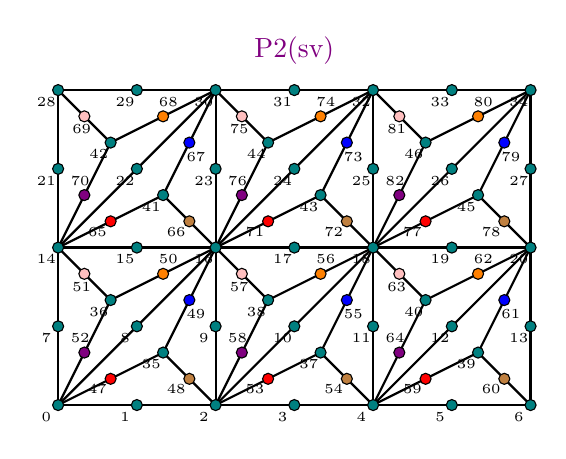
\begin{tikzpicture} 

%\draw[fill=gray!23,gray!23](0,0) rectangle (6,5);
%\draw[step=0.5cm,gray,very thin] (0,0) grid (6,4); %background grid

%ielx=1,iely=1,low
\draw[thick] (0,0)--(1.33333,0.66667);
\draw[thick] (2,0)--(1.33333,0.66667);
\draw[thick] (2,2)--(1.33333,0.66667);
%ielx=1,iely=1,high
\draw[thick] (0,0)--(0.666667,1.3333);
\draw[thick] (0,2)--(0.666667,1.3333);
\draw[thick] (2,2)--(0.666667,1.3333);

%ielx=2,iely=1,low
\draw[thick] (2,0)--(3.33333,0.66667);
\draw[thick] (4,0)--(3.33333,0.66667);
\draw[thick] (4,2)--(3.33333,0.66667);
%ielx=2,iely=1,high
\draw[thick] (2,0)--(2.666667,1.3333);
\draw[thick] (2,2)--(2.666667,1.3333);
\draw[thick] (4,2)--(2.666667,1.3333);

%ielx=2,iely=1,high
\draw[thick] (4,0)--(5.33333,0.66667);
\draw[thick] (6,0)--(5.33333,0.66667);
\draw[thick] (6,2)--(5.33333,0.66667);
%ielx=3,iely=1,high
\draw[thick] (4,0)--(4.666667,1.3333);
\draw[thick] (4,2)--(4.666667,1.3333);
\draw[thick] (6,2)--(4.666667,1.3333);

%ielx=1,iely=2,low
\draw[thick] (0,2)--(1.33333,2.66667);
\draw[thick] (2,2)--(1.33333,2.66667);
\draw[thick] (2,4)--(1.33333,2.66667);
%ielx=1,iely=1,high
\draw[thick] (0,2)--(0.666667,3.3333);
\draw[thick] (0,4)--(0.666667,3.3333);
\draw[thick] (2,4)--(0.666667,3.3333);


%ielx=2,iely=1,low
\draw[thick] (2,2)--(3.33333,2.66667);
\draw[thick] (4,2)--(3.33333,2.66667);
\draw[thick] (4,4)--(3.33333,2.66667);
%ielx=2,iely=1,high
\draw[thick] (2,2)--(2.666667,3.3333);
\draw[thick] (2,4)--(2.666667,3.3333);
\draw[thick] (4,4)--(2.666667,3.3333);

%ielx=2,iely=1,high
\draw[thick] (4,2)--(5.33333,2.66667);
\draw[thick] (6,2)--(5.33333,2.66667);
\draw[thick] (6,4)--(5.33333,2.66667);
%ielx=3,iely=1,high
\draw[thick] (4,2)--(4.666667,3.3333);
\draw[thick] (4,4)--(4.666667,3.3333);
\draw[thick] (6,4)--(4.666667,3.3333);





\node[violet] at (3,4.5) {P2(sv)}; 
\draw[thick] (0,0) -- (6,0) -- (6,4) -- (0,4) -- cycle; 
\draw[thick] (0,2) -- (6,2) ; 
\draw[thick] (2,0) -- (2,4) ; 
\draw[thick] (4,0) -- (4,4) ; 
\draw[thick] (0,2) -- (2,4) ; %diag
\draw[thick] (0,0) -- (4,4) ; %diag
\draw[thick] (2,0) -- (6,4) ; %diag
\draw[thick] (4,0) -- (6,2) ; %diag

%\draw[thick] (6,0) -- (4,2) -- (6,4) ; 
\draw[black,fill=teal] ( 0.000000 , 0.000000)     circle (2pt); 
\node[] at ( -0.150000, -0.150000 ) {\tiny 0 }; 
\draw[black,fill=teal] ( 1.000000 , 0.000000)     circle (2pt); 
\node[] at ( 0.850000, -0.150000 ) {\tiny 1 }; 
\draw[black,fill=teal] ( 2.000000 , 0.000000)     circle (2pt); 
\node[] at ( 1.850000, -0.150000 ) {\tiny 2 }; 
\draw[black,fill=teal] ( 3.000000 , 0.000000)     circle (2pt); 
\node[] at ( 2.850000, -0.150000 ) {\tiny 3 }; 
\draw[black,fill=teal] ( 4.000000 , 0.000000)     circle (2pt); 
\node[] at ( 3.850000, -0.150000 ) {\tiny 4 }; 
\draw[black,fill=teal] ( 5.000000 , 0.000000)     circle (2pt); 
\node[] at ( 4.850000, -0.150000 ) {\tiny 5 }; 
\draw[black,fill=teal] ( 6.000000 , 0.000000)     circle (2pt); 
\node[] at ( 5.850000, -0.150000 ) {\tiny 6 }; 
\draw[black,fill=teal] ( 0.000000 , 1.000000)     circle (2pt); 
\node[] at ( -0.150000, 0.850000 ) {\tiny 7 }; 
\draw[black,fill=teal] ( 1.000000 , 1.000000)     circle (2pt); 
\node[] at ( 0.850000, 0.850000 ) {\tiny 8 }; 
\draw[black,fill=teal] ( 2.000000 , 1.000000)     circle (2pt); 
\node[] at ( 1.850000, 0.850000 ) {\tiny 9 }; 
\draw[black,fill=teal] ( 3.000000 , 1.000000)     circle (2pt); 
\node[] at ( 2.850000, 0.850000 ) {\tiny 10 }; 
\draw[black,fill=teal] ( 4.000000 , 1.000000)     circle (2pt); 
\node[] at ( 3.850000, 0.850000 ) {\tiny 11 }; 
\draw[black,fill=teal] ( 5.000000 , 1.000000)     circle (2pt); 
\node[] at ( 4.850000, 0.850000 ) {\tiny 12 }; 
\draw[black,fill=teal] ( 6.000000 , 1.000000)     circle (2pt); 
\node[] at ( 5.850000, 0.850000 ) {\tiny 13 }; 
\draw[black,fill=teal] ( 0.000000 , 2.000000)     circle (2pt); 
\node[] at ( -0.150000, 1.850000 ) {\tiny 14 }; 
\draw[black,fill=teal] ( 1.000000 , 2.000000)     circle (2pt); 
\node[] at ( 0.850000, 1.850000 ) {\tiny 15 }; 
\draw[black,fill=teal] ( 2.000000 , 2.000000)     circle (2pt); 
\node[] at ( 1.850000, 1.850000 ) {\tiny 16 }; 
\draw[black,fill=teal] ( 3.000000 , 2.000000)     circle (2pt); 
\node[] at ( 2.850000, 1.850000 ) {\tiny 17 }; 
\draw[black,fill=teal] ( 4.000000 , 2.000000)     circle (2pt); 
\node[] at ( 3.850000, 1.850000 ) {\tiny 18 }; 
\draw[black,fill=teal] ( 5.000000 , 2.000000)     circle (2pt); 
\node[] at ( 4.850000, 1.850000 ) {\tiny 19 }; 
\draw[black,fill=teal] ( 6.000000 , 2.000000)     circle (2pt); 
\node[] at ( 5.850000, 1.850000 ) {\tiny 20 }; 
\draw[black,fill=teal] ( 0.000000 , 3.000000)     circle (2pt); 
\node[] at ( -0.150000, 2.850000 ) {\tiny 21 }; 
\draw[black,fill=teal] ( 1.000000 , 3.000000)     circle (2pt); 
\node[] at ( 0.850000, 2.850000 ) {\tiny 22 }; 
\draw[black,fill=teal] ( 2.000000 , 3.000000)     circle (2pt); 
\node[] at ( 1.850000, 2.850000 ) {\tiny 23 }; 
\draw[black,fill=teal] ( 3.000000 , 3.000000)     circle (2pt); 
\node[] at ( 2.850000, 2.850000 ) {\tiny 24 }; 
\draw[black,fill=teal] ( 4.000000 , 3.000000)     circle (2pt); 
\node[] at ( 3.850000, 2.850000 ) {\tiny 25 }; 
\draw[black,fill=teal] ( 5.000000 , 3.000000)     circle (2pt); 
\node[] at ( 4.850000, 2.850000 ) {\tiny 26 }; 
\draw[black,fill=teal] ( 6.000000 , 3.000000)     circle (2pt); 
\node[] at ( 5.850000, 2.850000 ) {\tiny 27 }; 
\draw[black,fill=teal] ( 0.000000 , 4.000000)     circle (2pt); 
\node[] at ( -0.150000, 3.850000 ) {\tiny 28 }; 
\draw[black,fill=teal] ( 1.000000 , 4.000000)     circle (2pt); 
\node[] at ( 0.850000, 3.850000 ) {\tiny 29 }; 
\draw[black,fill=teal] ( 2.000000 , 4.000000)     circle (2pt); 
\node[] at ( 1.850000, 3.850000 ) {\tiny 30 }; 
\draw[black,fill=teal] ( 3.000000 , 4.000000)     circle (2pt); 
\node[] at ( 2.850000, 3.850000 ) {\tiny 31 }; 
\draw[black,fill=teal] ( 4.000000 , 4.000000)     circle (2pt); 
\node[] at ( 3.850000, 3.850000 ) {\tiny 32 }; 
\draw[black,fill=teal] ( 5.000000 , 4.000000)     circle (2pt); 
\node[] at ( 4.850000, 3.850000 ) {\tiny 33 }; 
\draw[black,fill=teal] ( 6.000000 , 4.000000)     circle (2pt); 
\node[] at ( 5.850000, 3.850000 ) {\tiny 34 }; 

\draw[black,fill=teal] ( 1.333333 , 0.666667)     circle (2pt); 
\node[] at ( 1.183333, 0.516667 ) {\tiny 35 }; 
\draw[black,fill=teal] ( 0.666667 , 1.333333)     circle (2pt); 
\node[] at ( 0.516667, 1.183333 ) {\tiny 36 }; 
\draw[black,fill=teal] ( 3.333333 , 0.666667)     circle (2pt); 
\node[] at ( 3.183333, 0.516667 ) {\tiny 37 }; 
\draw[black,fill=teal] ( 2.666667 , 1.333333)     circle (2pt); 
\node[] at ( 2.516667, 1.183333 ) {\tiny 38 }; 
\draw[black,fill=teal] ( 5.333333 , 0.666667)     circle (2pt); 
\node[] at ( 5.183333, 0.516667 ) {\tiny 39 }; 
\draw[black,fill=teal] ( 4.666667 , 1.333333)     circle (2pt); 
\node[] at ( 4.516667, 1.183333 ) {\tiny 40 }; 

\draw[black,fill=teal] ( 1.333333 , 2.666667)     circle (2pt); 
\node[] at ( 1.183333, 2.516667 ) {\tiny 41 }; 
\draw[black,fill=teal] ( 0.666667 , 3.333333)     circle (2pt); 
\node[] at ( 0.516667, 3.183333 ) {\tiny 42 }; 
\draw[black,fill=teal] ( 3.333333 , 2.666667)     circle (2pt); 
\node[] at ( 3.183333, 2.516667 ) {\tiny 43 }; 
\draw[black,fill=teal] ( 2.666667 , 3.333333)     circle (2pt); 
\node[] at ( 2.516667, 3.183333 ) {\tiny 44 }; 
\draw[black,fill=teal] ( 5.333333 , 2.666667)     circle (2pt); 
\node[] at ( 5.183333, 2.516667 ) {\tiny 45 }; 
\draw[black,fill=teal] ( 4.666667 , 3.333333)     circle (2pt); 
\node[] at ( 4.516667, 3.183333 ) {\tiny 46 }; 

\draw[black,fill=red] ( 0.666667 , 0.3333)     circle (2pt); 
\node[] at ( 0.5, 0.2 ) {\tiny 47 }; 
\draw[black,fill=red] ( 2.666667 , 0.3333)     circle (2pt); 
\node[] at ( 2.5, 0.2 ) {\tiny 53 }; 
\draw[black,fill=red] ( 4.666667 , 0.3333)     circle (2pt); 
\node[] at ( 4.5, 0.2 ) {\tiny 59 }; 
\draw[black,fill=red] ( 0.666667 , 2.3333)     circle (2pt); 
\node[] at ( 0.5, 2.2 ) {\tiny 65 }; 
\draw[black,fill=red] ( 2.666667 , 2.3333)     circle (2pt); 
\node[] at ( 2.5, 2.2 ) {\tiny 71 }; 
\draw[black,fill=red] ( 4.666667 , 2.3333)     circle (2pt); 
\node[] at ( 4.5, 2.2 ) {\tiny 77 }; 

\draw[black,fill=brown] ( 1.6667 , 0.3333)     circle (2pt); 
\node[] at ( 1.5, 0.2 ) {\tiny 48 }; 
\draw[black,fill=brown] ( 3.6667 , 0.3333)     circle (2pt); 
\node[] at ( 3.5, 0.2 ) {\tiny 54 }; 
\draw[black,fill=brown] ( 5.6667 , 0.3333)     circle (2pt); 
\node[] at ( 5.5, 0.2 ) {\tiny 60 }; 
\draw[black,fill=brown] ( 1.6667 , 2.3333)     circle (2pt); 
\node[] at ( 1.5, 2.2 ) {\tiny 66 }; 
\draw[black,fill=brown] ( 3.6667 , 2.3333)     circle (2pt); 
\node[] at ( 3.5, 2.2 ) {\tiny 72 }; 
\draw[black,fill=brown] ( 5.6667 , 2.3333)     circle (2pt); 
\node[] at ( 5.5, 2.2 ) {\tiny 78 }; 

\draw[black,fill=blue] ( 1.6667 , 1.3333)     circle (2pt); 
\node[] at ( 1.75, 1.15 ) {\tiny 49 }; 
\draw[black,fill=blue] ( 3.6667 , 1.3333)     circle (2pt); 
\node[] at ( 3.75, 1.15 ) {\tiny 55 }; 
\draw[black,fill=blue] ( 5.6667 , 1.3333)     circle (2pt); 
\node[] at ( 5.75, 1.15 ) {\tiny 61 }; 
\draw[black,fill=blue] ( 1.6667 , 3.3333)     circle (2pt); 
\node[] at ( 1.75, 3.15 ) {\tiny 67 }; 
\draw[black,fill=blue] ( 3.6667 , 3.3333)     circle (2pt); 
\node[] at ( 3.75, 3.15 ) {\tiny 73 }; 
\draw[black,fill=blue] ( 5.6667 , 3.3333)     circle (2pt); 
\node[] at ( 5.75, 3.15 ) {\tiny 79 }; 

\draw[black,fill=violet] ( 0.3333,0.666667)     circle (2pt); 
\node[] at ( 1.4,1.85 ) {\tiny 50 }; 
\draw[black,fill=violet] ( 2.3333,0.666667)     circle (2pt); 
\node[] at ( 3.4,1.85 ) {\tiny 56 }; 
\draw[black,fill=violet] ( 4.3333,0.666667)     circle (2pt); 
\node[] at ( 5.4,1.85 ) {\tiny 62 }; 
\draw[black,fill=violet] ( 0.3333,2.666667)     circle (2pt); 
\node[] at ( 1.4,3.85 ) {\tiny 68 }; 
\draw[black,fill=violet] ( 2.3333,2.666667)     circle (2pt); 
\node[] at ( 3.4,3.85 ) {\tiny 74 }; 
\draw[black,fill=violet] ( 4.3333,2.666667)     circle (2pt); 
\node[] at ( 5.4,3.85 ) {\tiny 80 }; 

\draw[black,fill=pink] ( 0.3333, 1.6667)     circle (2pt); 
\node[] at ( 0.3,1.5 ) {\tiny 51 }; 
\draw[black,fill=pink] ( 2.3333, 1.6667)     circle (2pt); 
\node[] at ( 2.3,1.5 ) {\tiny 57 }; 
\draw[black,fill=pink] ( 4.3333, 1.6667)     circle (2pt); 
\node[] at ( 4.3,1.5 ) {\tiny 63 }; 
\draw[black,fill=pink] ( 0.3333, 3.6667)     circle (2pt); 
\node[] at ( 0.3,3.5 ) {\tiny 69 }; 
\draw[black,fill=pink] ( 2.3333, 3.6667)     circle (2pt); 
\node[] at ( 2.3,3.5 ) {\tiny 75 }; 
\draw[black,fill=pink] ( 4.3333, 3.6667)     circle (2pt); 
\node[] at ( 4.3,3.5 ) {\tiny 81 }; 

\draw[black,fill=orange] ( 1.3333, 1.6667)     circle (2pt); 
\node[] at ( 0.28,0.85 ) {\tiny 52 }; 
\draw[black,fill=orange] ( 3.3333, 1.6667)     circle (2pt); 
\node[] at ( 2.28,0.85 ) {\tiny 58 }; 
\draw[black,fill=orange] ( 5.3333, 1.6667)     circle (2pt); 
\node[] at ( 4.28,0.85 ) {\tiny 64 }; 
\draw[black,fill=orange] ( 1.3333, 3.6667)     circle (2pt); 
\node[] at ( 0.28,2.85 ) {\tiny 70 }; 
\draw[black,fill=orange] ( 3.3333, 3.6667)     circle (2pt); 
\node[] at ( 2.28,2.85 ) {\tiny 76 }; 
\draw[black,fill=orange] ( 5.3333, 3.6667)     circle (2pt); 
\node[] at ( 4.28,2.85 ) {\tiny 82 }; 


\end{tikzpicture} 
\end{center} 


%\begin{tiny}
%\verbatiminput{python_codes/fieldstone_120/spaces/iconV_elt1_Han.ascii}
%\end{tiny}
\end{multicols}

%------------------
\begin{multicols}{2}

\begin{center} 
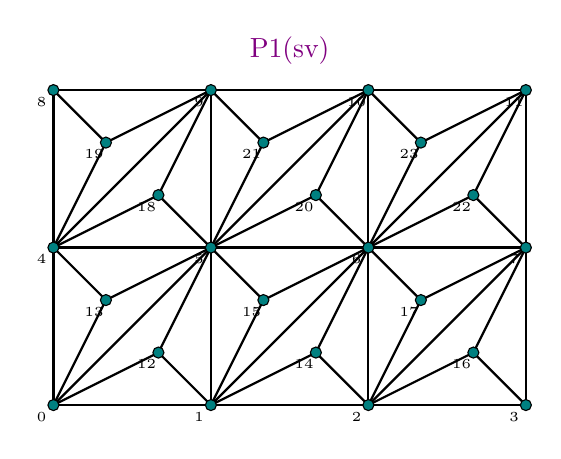
\begin{tikzpicture} 

%\draw[fill=gray!23,gray!23](0,0) rectangle (6,5);
%\draw[step=0.5cm,gray,very thin] (0,0) grid (6,4); %background grid

%ielx=1,iely=1,low
\draw[thick] (0,0)--(1.33333,0.66667);
\draw[thick] (2,0)--(1.33333,0.66667);
\draw[thick] (2,2)--(1.33333,0.66667);
%ielx=1,iely=1,high
\draw[thick] (0,0)--(0.666667,1.3333);
\draw[thick] (0,2)--(0.666667,1.3333);
\draw[thick] (2,2)--(0.666667,1.3333);

%ielx=2,iely=1,low
\draw[thick] (2,0)--(3.33333,0.66667);
\draw[thick] (4,0)--(3.33333,0.66667);
\draw[thick] (4,2)--(3.33333,0.66667);
%ielx=2,iely=1,high
\draw[thick] (2,0)--(2.666667,1.3333);
\draw[thick] (2,2)--(2.666667,1.3333);
\draw[thick] (4,2)--(2.666667,1.3333);

%ielx=2,iely=1,high
\draw[thick] (4,0)--(5.33333,0.66667);
\draw[thick] (6,0)--(5.33333,0.66667);
\draw[thick] (6,2)--(5.33333,0.66667);
%ielx=3,iely=1,high
\draw[thick] (4,0)--(4.666667,1.3333);
\draw[thick] (4,2)--(4.666667,1.3333);
\draw[thick] (6,2)--(4.666667,1.3333);

%ielx=1,iely=2,low
\draw[thick] (0,2)--(1.33333,2.66667);
\draw[thick] (2,2)--(1.33333,2.66667);
\draw[thick] (2,4)--(1.33333,2.66667);
%ielx=1,iely=1,high
\draw[thick] (0,2)--(0.666667,3.3333);
\draw[thick] (0,4)--(0.666667,3.3333);
\draw[thick] (2,4)--(0.666667,3.3333);


%ielx=2,iely=1,low
\draw[thick] (2,2)--(3.33333,2.66667);
\draw[thick] (4,2)--(3.33333,2.66667);
\draw[thick] (4,4)--(3.33333,2.66667);
%ielx=2,iely=1,high
\draw[thick] (2,2)--(2.666667,3.3333);
\draw[thick] (2,4)--(2.666667,3.3333);
\draw[thick] (4,4)--(2.666667,3.3333);

%ielx=2,iely=1,high
\draw[thick] (4,2)--(5.33333,2.66667);
\draw[thick] (6,2)--(5.33333,2.66667);
\draw[thick] (6,4)--(5.33333,2.66667);
%ielx=3,iely=1,high
\draw[thick] (4,2)--(4.666667,3.3333);
\draw[thick] (4,4)--(4.666667,3.3333);
\draw[thick] (6,4)--(4.666667,3.3333);





\node[violet] at (3,4.5) {P1(sv)}; 
\draw[thick] (0,0) -- (6,0) -- (6,4) -- (0,4) -- cycle; 
\draw[thick] (0,2) -- (6,2) ; 
\draw[thick] (2,0) -- (2,4) ; 
\draw[thick] (4,0) -- (4,4) ; 
\draw[thick] (0,2) -- (2,4) ; %diag
\draw[thick] (0,0) -- (4,4) ; %diag
\draw[thick] (2,0) -- (6,4) ; %diag
\draw[thick] (4,0) -- (6,2) ; %diag

%\draw[thick] (6,0) -- (4,2) -- (6,4) ; 
\draw[black,fill=teal] ( 0.000000 , 0.000000)     circle (2pt); 
\node[] at ( -0.150000, -0.150000 ) {\tiny 0 }; 
\draw[black,fill=teal] ( 2.000000 , 0.000000)     circle (2pt); 
\node[] at ( 1.850000, -0.150000 ) {\tiny 1 }; 
\draw[black,fill=teal] ( 4.000000 , 0.000000)     circle (2pt); 
\node[] at ( 3.850000, -0.150000 ) {\tiny 2 }; 
\draw[black,fill=teal] ( 6.000000 , 0.000000)     circle (2pt); 
\node[] at ( 5.850000, -0.150000 ) {\tiny 3 }; 
\draw[black,fill=teal] ( 0.000000 , 2.000000)     circle (2pt); 
\node[] at ( -0.150000, 1.850000 ) {\tiny 4 }; 
\draw[black,fill=teal] ( 2.000000 , 2.000000)     circle (2pt); 
\node[] at ( 1.850000, 1.850000 ) {\tiny 5 }; 
\draw[black,fill=teal] ( 4.000000 , 2.000000)     circle (2pt); 
\node[] at ( 3.850000, 1.850000 ) {\tiny 6 }; 
\draw[black,fill=teal] ( 6.000000 , 2.000000)     circle (2pt); 
\node[] at ( 5.850000, 1.850000 ) {\tiny 7 }; 
\draw[black,fill=teal] ( 0.000000 , 4.000000)     circle (2pt); 
\node[] at ( -0.150000, 3.850000 ) {\tiny 8 }; 
\draw[black,fill=teal] ( 2.000000 , 4.000000)     circle (2pt); 
\node[] at ( 1.850000, 3.850000 ) {\tiny 9 }; 
\draw[black,fill=teal] ( 4.000000 , 4.000000)     circle (2pt); 
\node[] at ( 3.850000, 3.850000 ) {\tiny 10 }; 
\draw[black,fill=teal] ( 6.000000 , 4.000000)     circle (2pt); 
\node[] at ( 5.850000, 3.850000 ) {\tiny 11 }; 

\draw[black,fill=teal] ( 1.333333 , 0.666667)     circle (2pt); 
\node[] at ( 1.183333, 0.516667 ) {\tiny 12 }; 
\draw[black,fill=teal] ( 0.666667 , 1.333333)     circle (2pt); 
\node[] at ( 0.516667, 1.183333 ) {\tiny 13 }; 
\draw[black,fill=teal] ( 3.333333 , 0.666667)     circle (2pt); 
\node[] at ( 3.183333, 0.516667 ) {\tiny 14 }; 
\draw[black,fill=teal] ( 2.666667 , 1.333333)     circle (2pt); 
\node[] at ( 2.516667, 1.183333 ) {\tiny 15 }; 
\draw[black,fill=teal] ( 5.333333 , 0.666667)     circle (2pt); 
\node[] at ( 5.183333, 0.516667 ) {\tiny 16 }; 
\draw[black,fill=teal] ( 4.666667 , 1.333333)     circle (2pt); 
\node[] at ( 4.516667, 1.183333 ) {\tiny 17 }; 

\draw[black,fill=teal] ( 1.333333 , 2.666667)     circle (2pt); 
\node[] at ( 1.183333, 2.516667 ) {\tiny 18 }; 
\draw[black,fill=teal] ( 0.666667 , 3.333333)     circle (2pt); 
\node[] at ( 0.516667, 3.183333 ) {\tiny 19 }; 
\draw[black,fill=teal] ( 3.333333 , 2.666667)     circle (2pt); 
\node[] at ( 3.183333, 2.516667 ) {\tiny 20 }; 
\draw[black,fill=teal] ( 2.666667 , 3.333333)     circle (2pt); 
\node[] at ( 2.516667, 3.183333 ) {\tiny 21 }; 
\draw[black,fill=teal] ( 5.333333 , 2.666667)     circle (2pt); 
\node[] at ( 5.183333, 2.516667 ) {\tiny 22 }; 
\draw[black,fill=teal] ( 4.666667 , 3.333333)     circle (2pt); 
\node[] at ( 4.516667, 3.183333 ) {\tiny 23 }; 

\end{tikzpicture} 
\end{center} 



%\begin{tiny}
%\verbatiminput{python_codes/fieldstone_120/spaces/iconV_elt1_Han.ascii}
%\end{tiny}
\end{multicols}











\newpage
%%%%%%%%%%%%%%%%%%%%%%%%%%%%%%%%%%%%%%%%%%%%%%%%%%%%%%%%%%%%%%%%%%%%%%%%%%%%%%%
%%%%%%%%%%%%%%%%%%%%%%%%%%%%%%%%%%%%%%%%%%%%%%%%%%%%%%%%%%%%%%%%%%%%%%%%%%%%%%%
\section*{Pressure normalisation for augmented Taylor-Hood elements}


I tried both ${\bm P}_2\times (P_1+P_0)$ and ${\bm Q}_2\times (Q_1+Q_0)$ on different manufactured solutions 
and I observed for both that the pressure I obtained visually consisted of 2 fields: (for quads) 
the continuous $Q_1$ which looked similar to the expected analytical field although offset by what 
seemed a constant (bottom green points), and the $Q_0$ field (top green points) which was 
very different than the $Q_1$ pressure:

\begin{center}
\includegraphics[width=7cm]{python_codes/fieldstone_120/images/q2q1q0pb}
\end{center}

I of course make sure in my code that the pressure fulfills $\int p dV=0$ but since 
the global constant function $p=constant$ is both in the $Q_1$ and $Q_0$ spaces the 
resulting normalised pressure was never good (see green line on plot below). 
This got me thinking about the '2 hydrostatic modes' of Gresho \& Sani and
I ended up looking at pressure normalisation in the following way (for quads again):
\begin{eqnarray}
0 
&=& \int_\Omega p dV \nn\\
&=& \sum_e \int_{\Omega_e} p dV \nn\\
&=& \sum_e \int_{\Omega_e} \left( \sum_{i=1}^5 \bN_i(x,y) p_i \right) dV \nn\\
&=& \sum_e \int_{\Omega_e} \left( \sum_{i=1}^4 \bN_i(x,y) p_i + \bN_5 p_5 \right) dV
\end{eqnarray}
with $\bN_{1,2,3,4}(r,s)=\frac14(1\pm r)(1\pm s)$ being
the $Q_1$ basis functions, $p_{1,2,3,4}$ the pressures at the corners
of the quad and $\bN_5(r,s)=1$ the $Q_0$ basis functions with $p_5$ the elemental pressure.
I then obtain 
\begin{eqnarray}
0 
&=& \underbrace{\sum_e \int_{\Omega_e} \left( \sum_{i=1}^4 \bN_i(x,y) p_i \right) dV}_{<p>_{Q_1}}
+ \underbrace{\sum_e \int_{\Omega_e} p_5  dV}_{<p>_{Q_0}}
\end{eqnarray}
and proceed to normalise the pressure by imposing both $<p>_{Q_1}=0$ and $<p>_{Q_0}=0$.
In this case the 'doubly normalised' pressure agrees with the analytical solution 
and I obtain the following error convergence plot:

\begin{center}
\includegraphics[width=6cm]{python_codes/fieldstone_120/images/q2q1q0}\\
{\captionfont 'doubly normalised' pressure error convergence is quadratic (blue line) and 
velocity error convergence is cubic (purple line). The green line is the 'wrong/raw' pressure. }
\end{center}




\newpage
%%%%%%%%%%%%%%%%%%%%%%%%%%%%%%%%%%%%%%%%%%%%%%%%%%%%%%%%%%%%%%%%%%%%%%%%%%%%%%%
%%%%%%%%%%%%%%%%%%%%%%%%%%%%%%%%%%%%%%%%%%%%%%%%%%%%%%%%%%%%%%%%%%%%%%%%%%%%%%%
\section*{Breakdown of the code}

One starts by loading the required finite element functions 
for the basis functions, the numerical quadrature and various tools:
\begin{lstlisting}
import FEbasis2D as FE
import FEquadrature as Q
import FEtools as Tools 
\end{lstlisting}

Then the desired setup/manufacture solution is imported, say:
\begin{lstlisting}
import mms_jolm17 as mms
\end{lstlisting}


The domain is a unit square:
\begin{lstlisting}
Lx=1
Ly=1
\end{lstlisting}

It is discretised by means of a $nelx\times nely$ cells. If quadrilateral 
elements are to be used then there are $nelx\times nely$ elements. If 
triangular elements are to be used then the cells are cut into two 
triangles and there are then $2\times nelx\times nely$ elements.

\begin{lstlisting}
nelx=16
\end{lstlisting}
In practice \lstinline{nely} is always set to the \lstinline{nelx} value.


%There are four boundaries to the domain (left, right, bottom and top). For the 
%benchmark under consideration we need to impose no slip boundary conditions 
%on all sides of the domain:
%\begin{lstlisting}
%left_bc  ='no_slip'
%right_bc ='no_slip'
%bottom_bc='no_slip'
%top_bc   ='no_slip'
%\end{lstlisting}

In two dimensions there are two velocity degrees of freedom per 
velocity node but only one pressure degree of freedom per pressure node:
\begin{lstlisting}
ndofV=2
ndofP=1
\end{lstlisting}

A finite element space must be assigned to both velocity and pressure. For example: 
\begin{lstlisting}
Vspace='Q2'
Pspace='Q1'
\end{lstlisting}

Whether a (bi-)linear mapping or isoparametric mapping is used is set with 
this parameter:
\begin{lstlisting}
isoparametric=False
\end{lstlisting}

Whether the mesh is randomized or not is set with 
\begin{lstlisting}
randomize_mesh=True
\end{lstlisting}

Whether the mesh structured or unstructured is set with 
\begin{lstlisting}
unstructured=0
\end{lstlisting}

A quadrature order must be assigned. If quadrilateral elements are used
this parameter is the number of quadrature points per dimension. 
If triangular elements are used it is the total number of quadrature points 
inside the element. For example: 
\begin{lstlisting}
nqpts=Q.nqpts_default(Vpsace)
\end{lstlisting}

For the chosen velocity and pressure spaces we retrieve the number of nodes 
('support points') inside an element.
\begin{lstlisting}
mV=FE.NNN_m(Vspace)
mP=FE.NNN_m(Pspace)
\end{lstlisting}

We then setup the quadrature rule for an element. This function 
returns the number of quadrature points inside the element, 
their coordinates in the $r,s$ space and their weights: 
\begin{lstlisting}
nqel,qcoords_r,qcoords_s,qweights=Q.quadrature(Vspace,nqpts)
\end{lstlisting}

The mesh is then created, or rather the meshes: one for the 
velocity nodes, one for the pressure nodes. They both count the 
same number of elements. There are \lstinline{NV} velocity nodes and their
coordinates are stored in the \lstinline{xV} and \lstinline{yV} arrays.
Likewise there are \lstinline{NP} pressure nodes and their
coordinates are stored in the \lstinline{xP} and \lstinline{yP} arrays. 

\begin{lstlisting}
if not unstructured:
   NV,nel,xV,yV,iconV=Tools.cartesian_mesh(Lx,Ly,nelx,nely,Vspace,mtype)
   NP,nel,xP,yP,iconP=Tools.cartesian_mesh(Lx,Ly,nelx,nely,Pspace,mtype)
else:
   nel,NV,NP,xV,yV,iconV,xP,yP,iconP=Tools.generate_random_mesh(Lx,nelx,\
                                                 Vspace,Pspace,experiment)  
\end{lstlisting}

Now that we know the number of elements and nodes we can compute the 
total number of quadrature points \lstinline{nq}, 
the total number of velocity dofs \lstinline{NfemV}, 
the total number of pressure dofs \lstinline{NfemP}, 
and the total number of dofs:

\begin{lstlisting}
nq=nqel*nel
NfemV=NV*ndofV
NfemP=NP*ndofP
Nfem=NfemV+NfemP
\end{lstlisting}

We will later need two arrays of size \lstinline{NfemV} (we are only imposing
velocity boundary conditions). \lstinline{bc_fix} is a boolean array.
We set \lstinline{bc_fix[i]=True} if the value of a given velocity dof \lstinline{i} is set. 
and the value of \lstinline{bc_val[i]} is the value of the desired boundary condition.

\begin{lstlisting}
bc_fix,bc_val=Tools.bc_setup(xV,yV,uth,vth,Lx,Ly,ndofV,mms.left_bc,mms.right_bc,mms.bottom_bc,mms.top_bc)
\end{lstlisting}

We then build the background mesh used for the mapping:
\begin{lstlisting}
space1=FE.mapping(Vspace)
m1=FE.NNN_m(space1)
N1,nel1,x1,y1,icon1=Tools.cartesian_mesh(Lx,Ly,nelx,nely,space1,mtype)
if randomize_mesh:
   hx=Lx/nelx
   hy=Ly/nely
   Tools.adapt_FE_mesh(x1,y1,icon1,m1,space1,xV,yV,iconV,nel,Vspace)
   Tools.adapt_FE_mesh(x1,y1,icon1,m1,space1,xP,yP,iconP,nel,Pspace)
\end{lstlisting}




Then we proceed to compute the volume of each element, i.e. 
\[
V_e = \int_{\Omega_e} dV = \sum_{iq=1}^{n_q} \omega_{i_q} |J_{i_q}|
\]
which translates as follows: 
\begin{lstlisting}
area=np.zeros(nel,dtype=np.float64) 
for iel in range(0,nel):
    for iq in range(0,nqel):
        rq=qcoords_r[iq]
        sq=qcoords_s[iq]
        weightq=qweights[iq]
        NNNV=FE.NNN(rq,sq,Vspace)
        xq=NNNV.dot(xV[iconV[:,iel]]) 
        yq=NNNV.dot(yV[iconV[:,iel]]) 
        dNNNVdr=FE.dNNNdr(rq,sq,Vspace)
        dNNNVds=FE.dNNNds(rq,sq,Vspace)
        if isoparametric:
           jcob,jcbi=Tools.J(mV,dNNNVdr,dNNNVds,xV[iconV[0:mV,iel]],yV[iconV[0:mV,iel]])
        else:
           dNNN1dr=FE.dNNNdr(rq,sq,space1)
           dNNN1ds=FE.dNNNds(rq,sq,space1)
           jcob,jcbi=Tools.J(m1,dNNN1dr,dNNN1ds,x1[icon1[0:m1,iel]],y1[icon1[0:m1,iel]])
        area[iel]+=jcob*weightq
\end{lstlisting}

\newpage
%=========================================
\section*{Examples of unstructured meshes}

\begin{center}
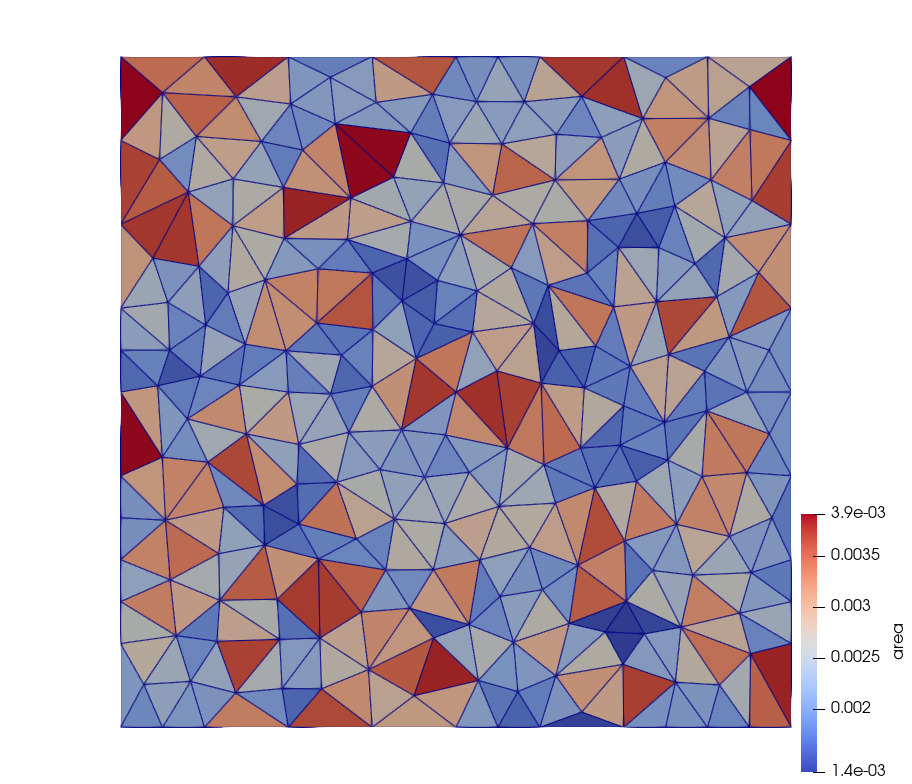
\includegraphics[width=5.7cm]{python_codes/fieldstone_120/images/unstructured16}
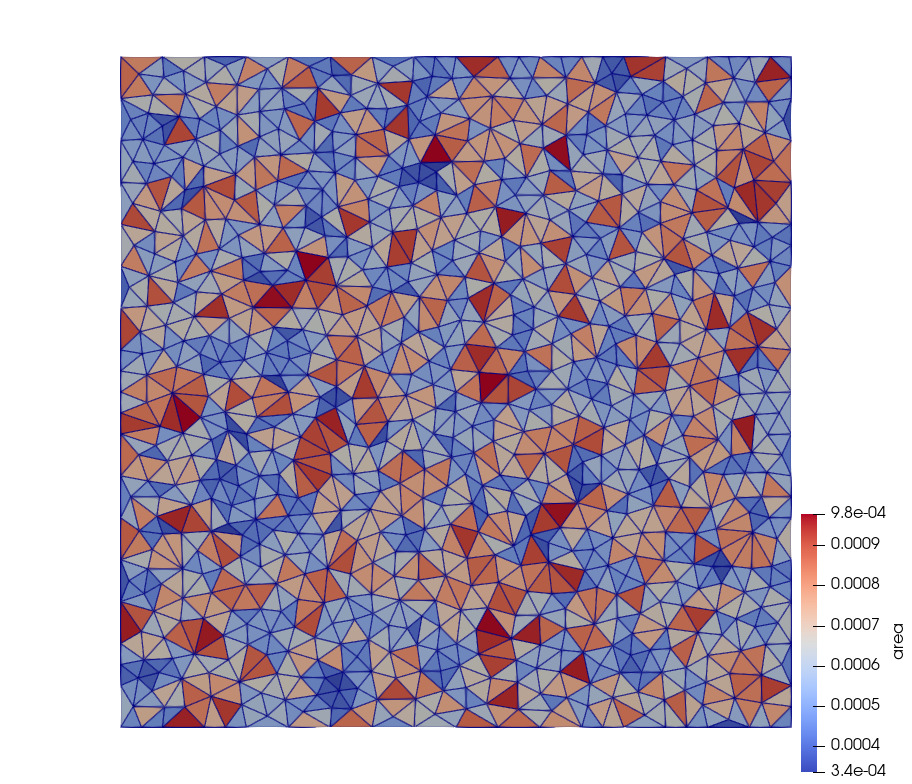
\includegraphics[width=5.7cm]{python_codes/fieldstone_120/images/unstructured32}\\
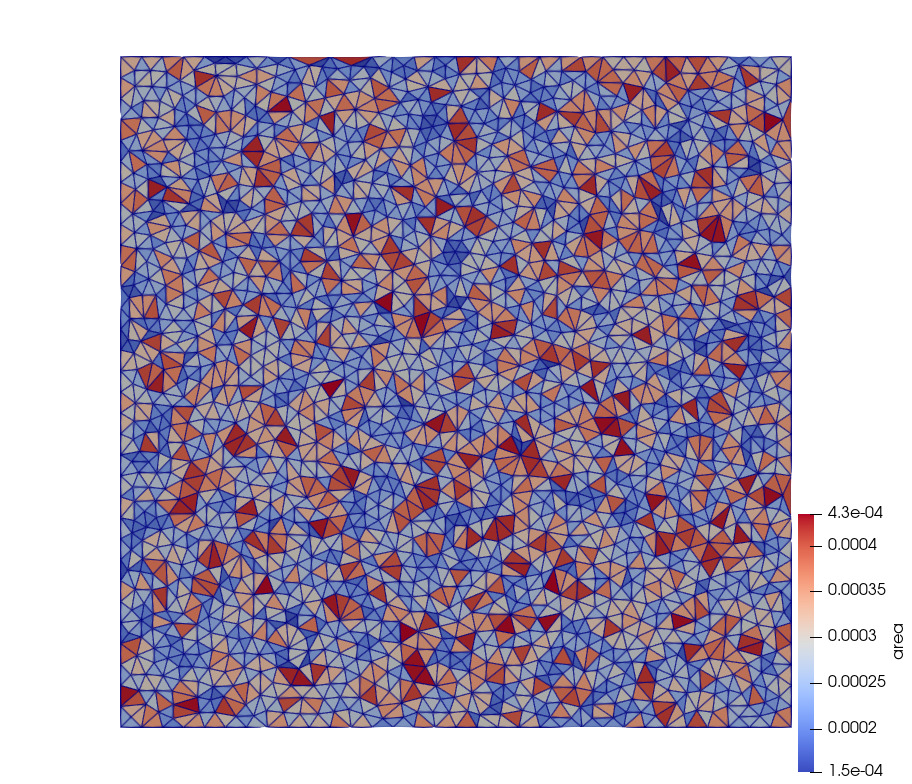
\includegraphics[width=5.7cm]{python_codes/fieldstone_120/images/unstructured48}
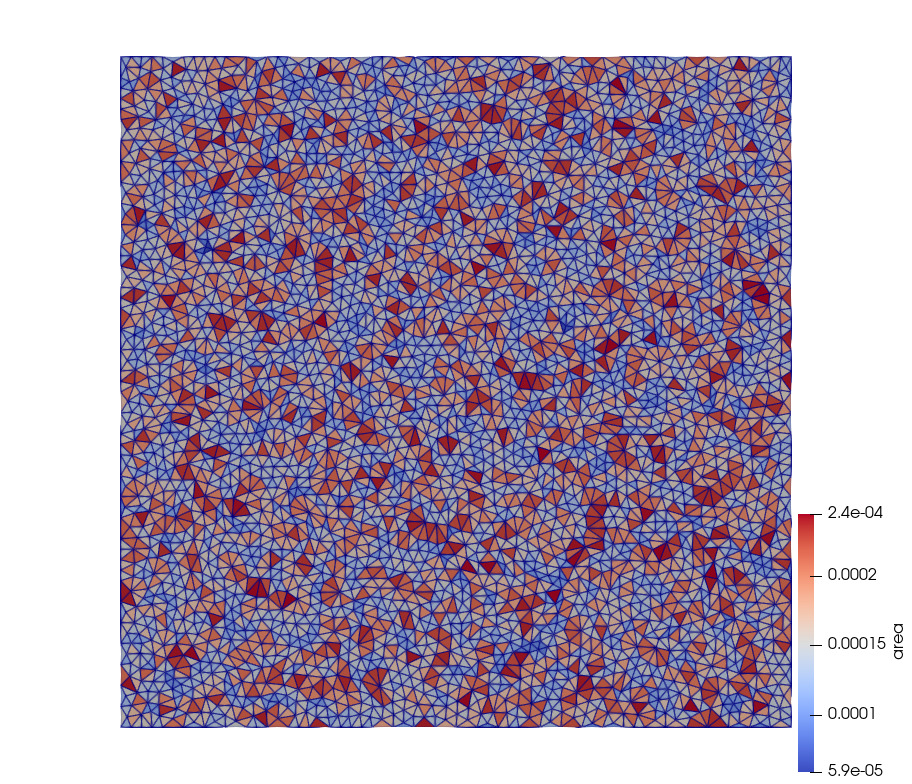
\includegraphics[width=5.7cm]{python_codes/fieldstone_120/images/unstructured64}
\end{center}


\newpage
%===============================================
\section*{Results - Donea \& Huerta (nov. 2024)}

{\tt script\_paper\_dh\_structured} and {\tt script\_paper\_dh\_unstructured}


%---------------------------
\subsection*{Structured mesh}

\begin{center}
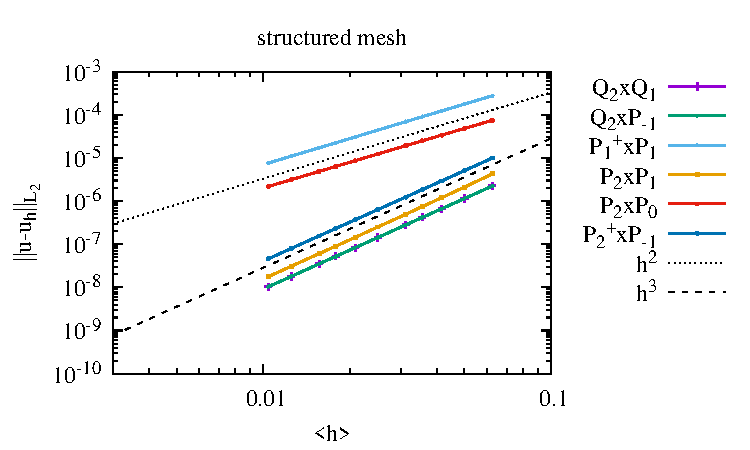
\includegraphics[width=5.7cm]{python_codes/fieldstone_120/paperresults/dh_structured_errorsV.pdf}
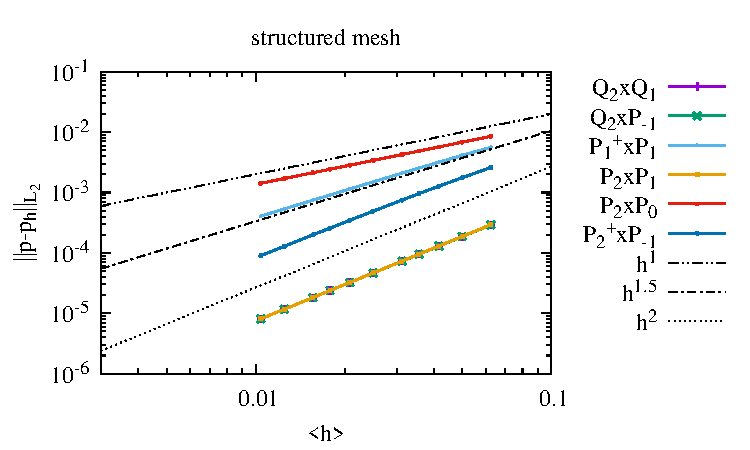
\includegraphics[width=5.7cm]{python_codes/fieldstone_120/paperresults/dh_structured_errorsP.pdf}
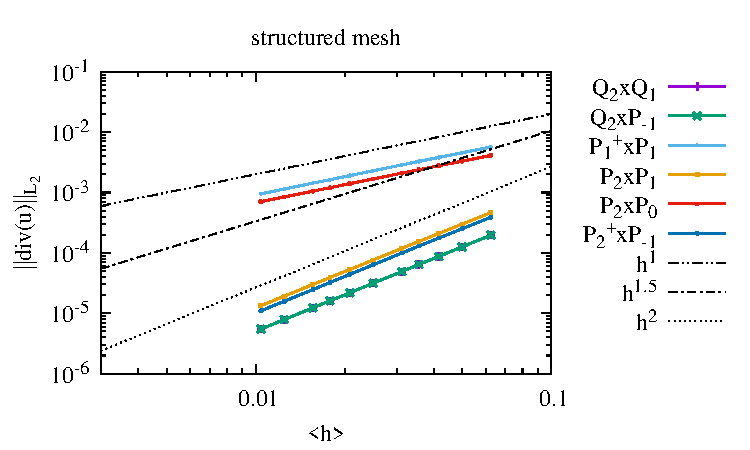
\includegraphics[width=5.7cm]{python_codes/fieldstone_120/paperresults/dh_structured_errors_divv.pdf}\\
\end{center}

\begin{center}
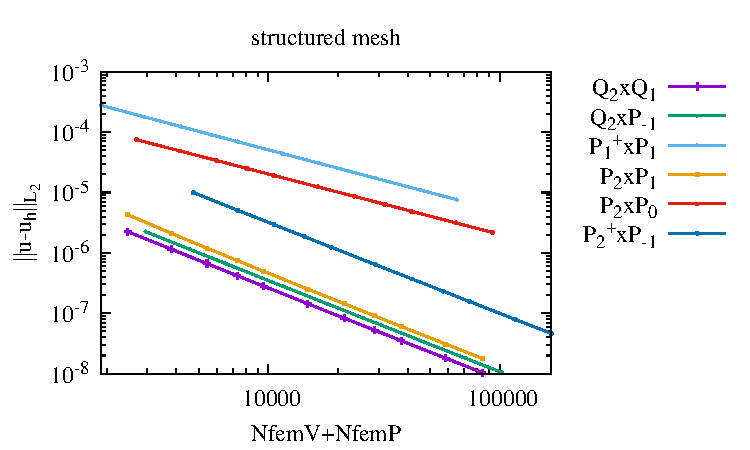
\includegraphics[width=5.7cm]{python_codes/fieldstone_120/paperresults/dh_structured_errorsV2.pdf}
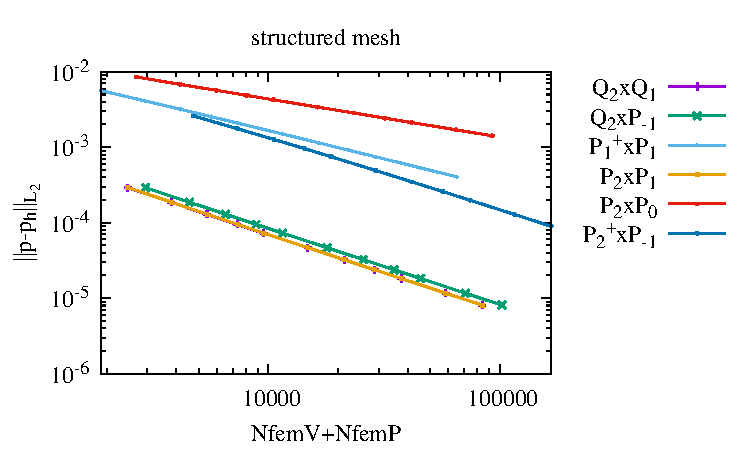
\includegraphics[width=5.7cm]{python_codes/fieldstone_120/paperresults/dh_structured_errorsP2.pdf}
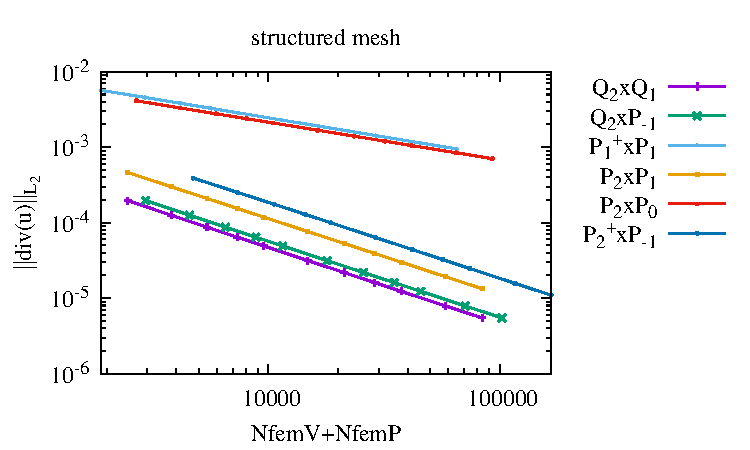
\includegraphics[width=5.7cm]{python_codes/fieldstone_120/paperresults/dh_structured_errors_divv2.pdf}\\
\end{center}

\begin{center}
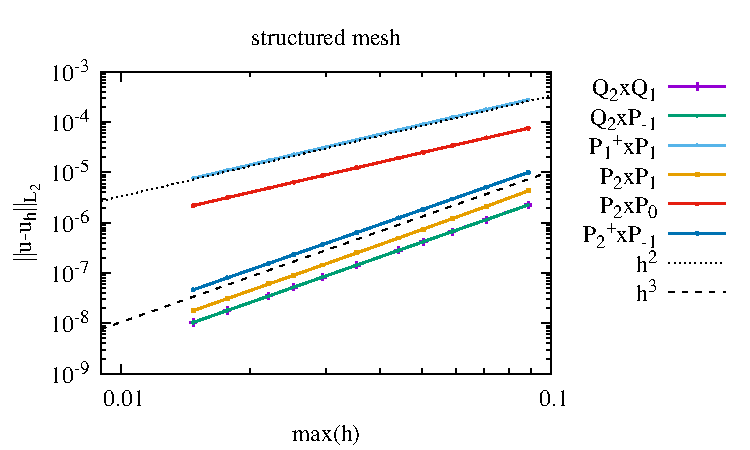
\includegraphics[width=5.7cm]{python_codes/fieldstone_120/paperresults/dh_structured_errorsV3.pdf}
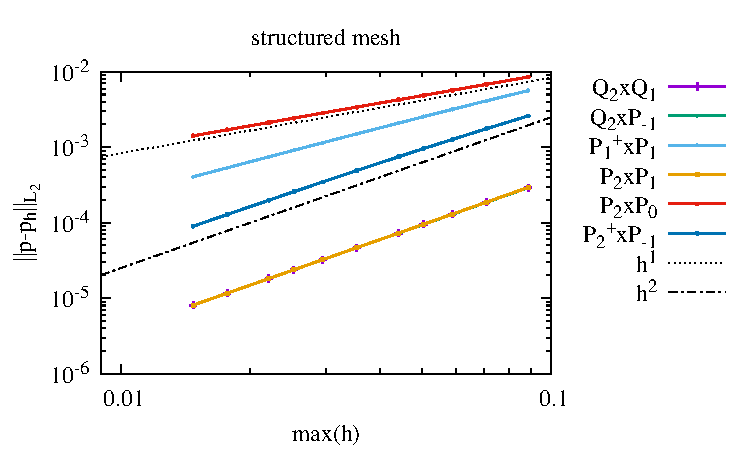
\includegraphics[width=5.7cm]{python_codes/fieldstone_120/paperresults/dh_structured_errorsP3.pdf}
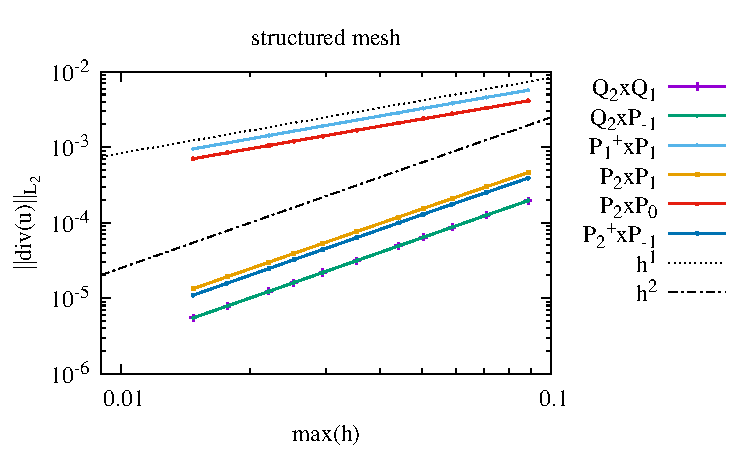
\includegraphics[width=5.7cm]{python_codes/fieldstone_120/paperresults/dh_structured_errors_divv3.pdf}\\
\end{center}

%---------------------------
\subsection*{Unstructured mesh}

\begin{center}
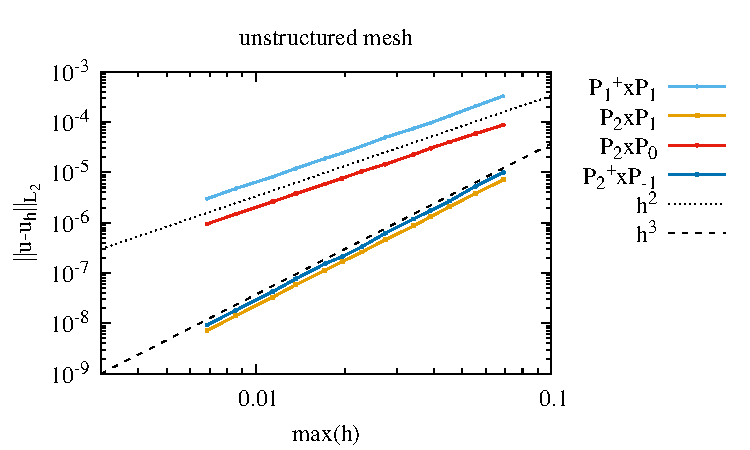
\includegraphics[width=5.7cm]{python_codes/fieldstone_120/paperresults/dh_unstructured_errorsV.pdf}
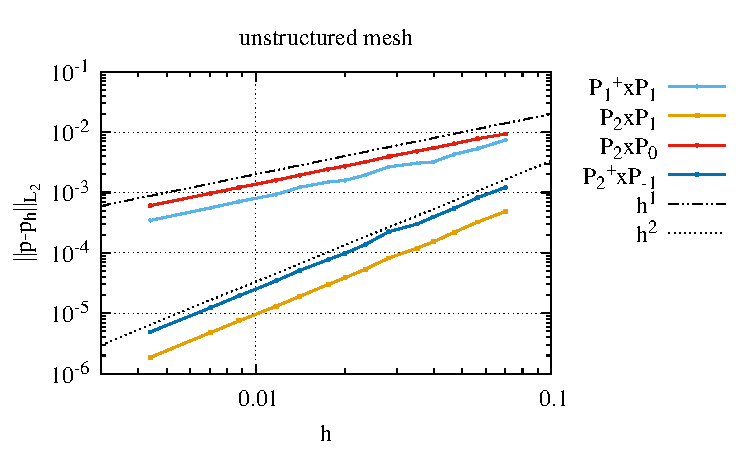
\includegraphics[width=5.7cm]{python_codes/fieldstone_120/paperresults/dh_unstructured_errorsP.pdf}
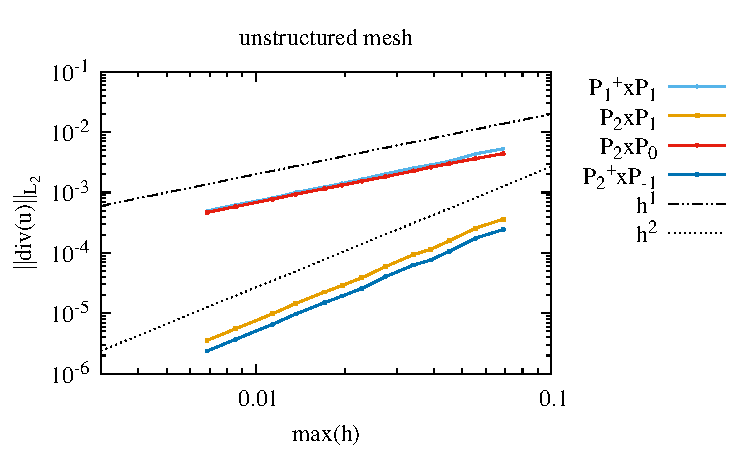
\includegraphics[width=5.7cm]{python_codes/fieldstone_120/paperresults/dh_unstructured_errors_divv.pdf}\\
\end{center}

\begin{center}
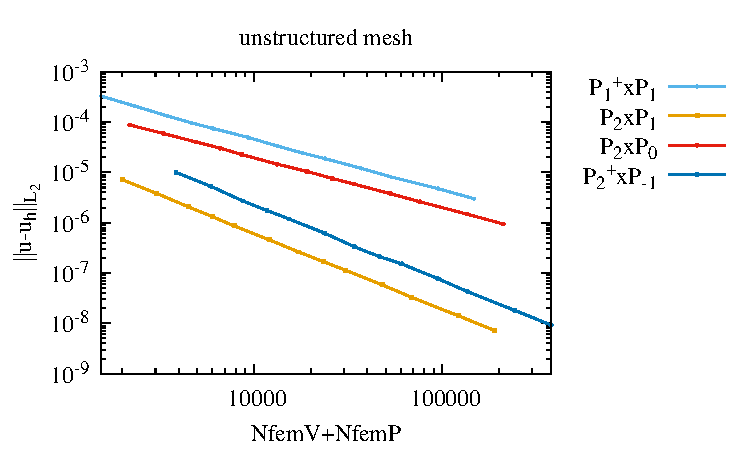
\includegraphics[width=5.7cm]{python_codes/fieldstone_120/paperresults/dh_unstructured_errorsV2.pdf}
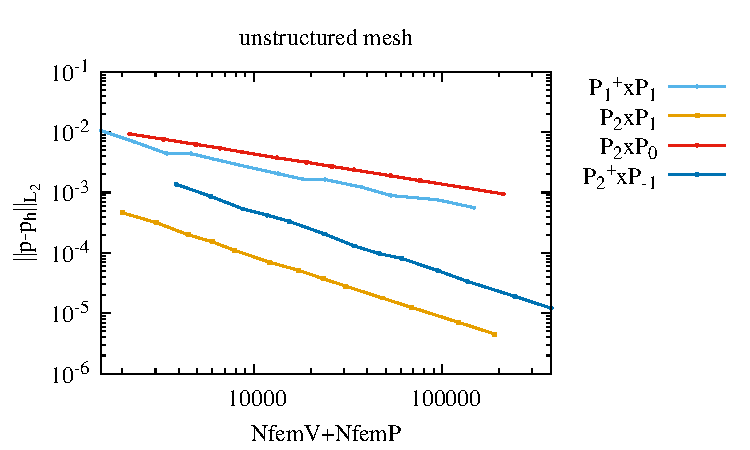
\includegraphics[width=5.7cm]{python_codes/fieldstone_120/paperresults/dh_unstructured_errorsP2.pdf}
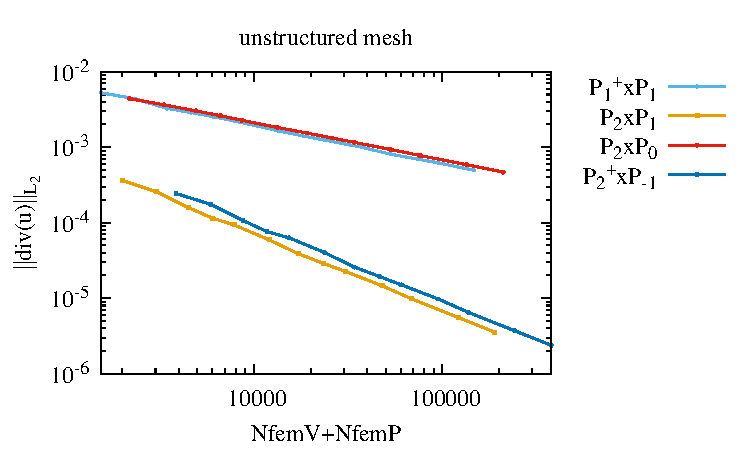
\includegraphics[width=5.7cm]{python_codes/fieldstone_120/paperresults/dh_unstructured_errors_divv2.pdf}\\
\end{center}

\begin{center}
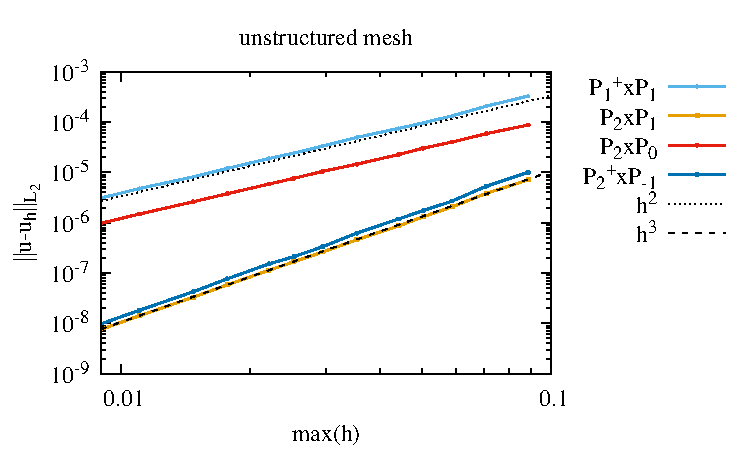
\includegraphics[width=5.7cm]{python_codes/fieldstone_120/paperresults/dh_unstructured_errorsV3.pdf}
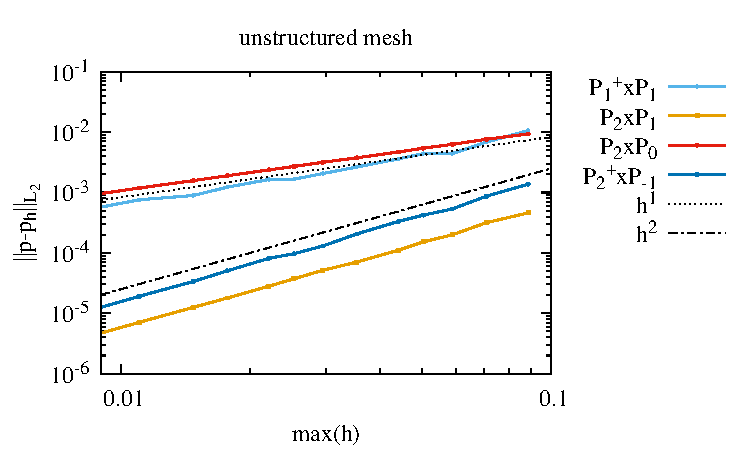
\includegraphics[width=5.7cm]{python_codes/fieldstone_120/paperresults/dh_unstructured_errorsP3.pdf}
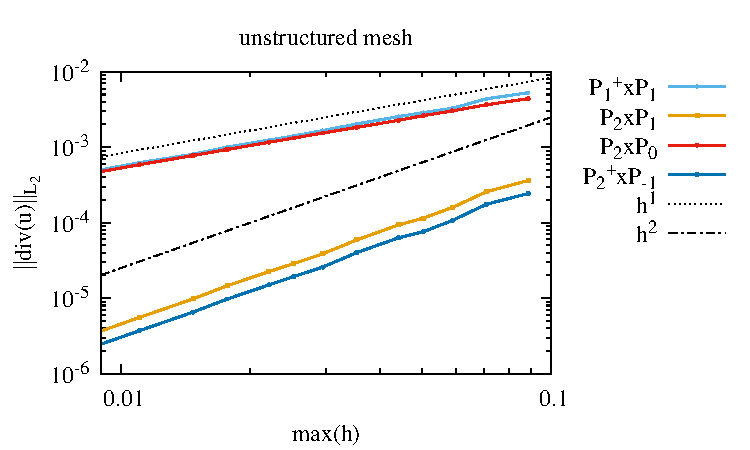
\includegraphics[width=5.7cm]{python_codes/fieldstone_120/paperresults/dh_unstructured_errors_divv3.pdf}\\
\end{center}






\newpage
%%%%%%%%%%%%%%%%%%%%%%%%%%%%%%%%%%%%%%%%%%%%%%%%%%%%%%%%%%%%%%%%%%%%%%%%%%%%%%%
\section*{NEW Results - SolKz}

{\tt script\_paper\_solkz\_structured} and {\tt script\_paper\_solkz\_unstructured}

\begin{center}
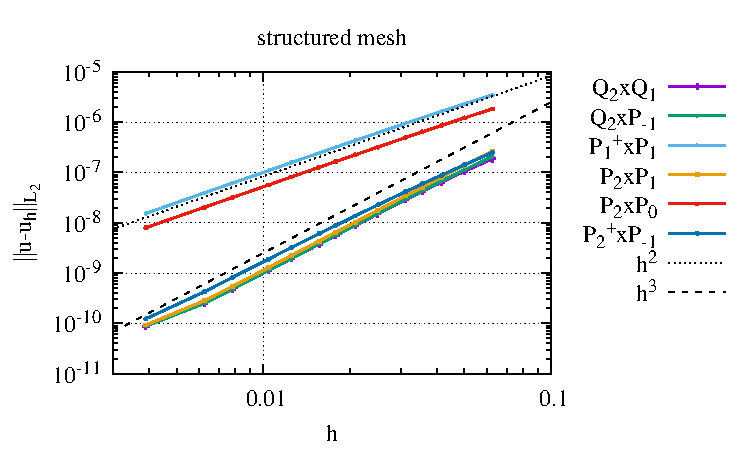
\includegraphics[width=8cm]{python_codes/fieldstone_120/paperresults/solkz_structured_errorsV.pdf}
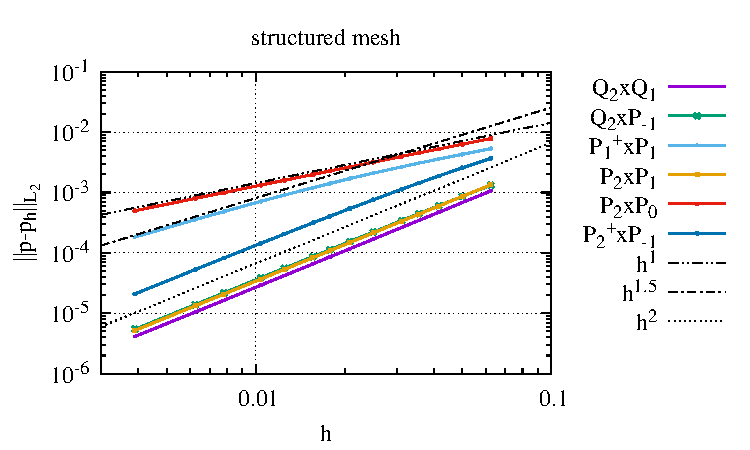
\includegraphics[width=8cm]{python_codes/fieldstone_120/paperresults/solkz_structured_errorsP.pdf}\\
\includegraphics[width=8cm]{python_codes/fieldstone_120/paperresults/solkz_unstructured_errorsV.pdf}
\includegraphics[width=8cm]{python_codes/fieldstone_120/paperresults/solkz_unstructured_errorsP.pdf}
\end{center}

\textcite{demh19} uses CR elements and report cubic convergence for velocity and quadratic for pressure.


\newpage
%%%%%%%%%%%%%%%%%%%%%%%%%%%%%%%%%%%%%%%%%%%%%%%%%%%%%%%%%%%%%%%%%%%%%%%%%%%%%%%
\section*{NEW Results - SolCx}

{\tt script\_paper\_solcx\_structured} and {\tt script\_paper\_solcx\_unstructured}

\begin{center}
\includegraphics[width=8cm]{python_codes/fieldstone_120/paperresults/solcx_structured_errorsV.pdf}
\includegraphics[width=8cm]{python_codes/fieldstone_120/paperresults/solcx_structured_errorsP.pdf}\\
\includegraphics[width=8cm]{python_codes/fieldstone_120/paperresults/solcx_unstructured_errorsV.pdf}
\includegraphics[width=8cm]{python_codes/fieldstone_120/paperresults/solcx_unstructured_errorsP.pdf}
\end{center}

\textcite{demh19} uses CR elements and also reports cubic convergence for velocity and quadratic for pressure
for both even and odd meshes

%\includegraphics[width=5.7cm]{python_codes/fieldstone_120/paperresults/solcx/unstructured/vel}
%\includegraphics[width=5.7cm]{python_codes/fieldstone_120/paperresults/solcx/unstructured/press}

\newpage
%%%%%%%%%%%%%%%%%%%%%%%%%%%%%%%%%%%%%%%%%%%%%%%%%%%%%%%%%%%%%%%%%%%%%%%%%%%%%%%
\section*{NEW Results - square sinker}

The domain is the unit square. Free-slip boundary conditions are applied on all 
four sides. The domain is filled with fluid with $\eta_f=1$ and $\rho_f=1$.
There is a square sinker in the middle of the domain of size $0.25\times 0.25$ with $\eta_s=100$ and
$\rho_s=1.001$. Gravity is set to $\vec{g}=-\vec{e}_y$. 
Resolutions \lstinline{nelx=16,32,64,128} are chosen so that element boundaries align with sinker boundaries 
(material averaging is then irrelevant, an element is either 100\% fluid or 100\% sinker material). 

%There is no analytical solution so by setting $\vec{\upnu}^{th}=\vec{0}$ and 
%$p^{th}=0$ the computed errors are in fact the vrms and prms shown hereunder.

Reported velocity is the root mean square velocity inside the whole block.
Reported pressure is the pressure(s) on the middle node of the block.

%-------------------------------
\subsubsection*{structured mesh}

{\tt script\_paper\_sinker}

\begin{center}
\includegraphics[width=4cm]{python_codes/fieldstone_120/paperresults/sinker/structured/vel.png}
\includegraphics[width=4cm]{python_codes/fieldstone_120/paperresults/sinker/structured/press.png}
\end{center}

\begin{center}
\includegraphics[width=7cm]{python_codes/fieldstone_120/paperresults/sinker/structured/sinker_vel_16}
\includegraphics[width=7cm]{python_codes/fieldstone_120/paperresults/sinker/structured/sinker_vel_32}\\
\includegraphics[width=7cm]{python_codes/fieldstone_120/paperresults/sinker/structured/sinker_vel_64}
\includegraphics[width=7cm]{python_codes/fieldstone_120/paperresults/sinker/structured/sinker_vel_128}\\
\includegraphics[width=7cm]{python_codes/fieldstone_120/paperresults/sinker/structured/sinker_press_16}
\includegraphics[width=7cm]{python_codes/fieldstone_120/paperresults/sinker/structured/sinker_press_32}\\
\includegraphics[width=7cm]{python_codes/fieldstone_120/paperresults/sinker/structured/sinker_press_64}
\includegraphics[width=7cm]{python_codes/fieldstone_120/paperresults/sinker/structured/sinker_press_128}
\end{center}


\newpage
%%%%%%%%%%%%%%%%%%%%%%%%%%%%%%%%%%%%%%%%%%%%%%%%%%%%%%%%%%%%%%%%%%%%%%%%%%%%%%%
\section*{NEW Results - square sinker (reduced density)}


%----------------------------
\subsection*{Structured mesh}

\begin{center}
\includegraphics[width=8cm]{python_codes/fieldstone_120/paperresults/sinker_reduced/structured/sinker_reduced_vel_16}
\includegraphics[width=8cm]{python_codes/fieldstone_120/paperresults/sinker_reduced/structured/sinker_reduced_vel_32}\\
\includegraphics[width=8cm]{python_codes/fieldstone_120/paperresults/sinker_reduced/structured/sinker_reduced_vel_64}
\includegraphics[width=8cm]{python_codes/fieldstone_120/paperresults/sinker_reduced/structured/sinker_reduced_vel_128}\\
\includegraphics[width=8cm]{python_codes/fieldstone_120/paperresults/sinker_reduced/structured/sinker_reduced_vel_160}\\
\includegraphics[width=8cm]{python_codes/fieldstone_120/paperresults/sinker_reduced/structured/sinker_reduced_press_16}
\includegraphics[width=8cm]{python_codes/fieldstone_120/paperresults/sinker_reduced/structured/sinker_reduced_press_32}\\
\includegraphics[width=8cm]{python_codes/fieldstone_120/paperresults/sinker_reduced/structured/sinker_reduced_press_64}
\includegraphics[width=8cm]{python_codes/fieldstone_120/paperresults/sinker_reduced/structured/sinker_reduced_press_128}\\
\includegraphics[width=8cm]{python_codes/fieldstone_120/paperresults/sinker_reduced/structured/sinker_reduced_press_160}\\
\end{center}




\newpage
%%%%%%%%%%%%%%%%%%%%%%%%%%%%%%%%%%%%%%%%%%%%%%%%%%%%%%%%%%%%%%%%%%%%%%%%%%%%%%%
\section*{NEW Results - SolVi}

%-------------------------------
\subsection*{structured mesh}

\begin{center}
\includegraphics[width=8cm]{python_codes/fieldstone_120/paperresults/solvi_structured_errorsV.pdf}
\includegraphics[width=8cm]{python_codes/fieldstone_120/paperresults/solvi_structured_errorsP.pdf}\\
\includegraphics[width=8cm]{python_codes/fieldstone_120/paperresults/solvi_p_profile_structured_32.pdf}
\includegraphics[width=8cm]{python_codes/fieldstone_120/paperresults/solvi_p_profile_structured_96.pdf}
\end{center}


%-------------------------------
\subsection*{unstructured mesh}

\begin{center}
\includegraphics[width=8cm]{python_codes/fieldstone_120/paperresults/solvi_unstructured_errorsV.pdf}
\includegraphics[width=8cm]{python_codes/fieldstone_120/paperresults/solvi_unstructured_errorsP.pdf}\\
\includegraphics[width=8cm]{python_codes/fieldstone_120/paperresults/solvi_p_profile_unstructured_32.pdf}
\includegraphics[width=8cm]{python_codes/fieldstone_120/paperresults/solvi_p_profile_unstructured_96.pdf}
\end{center}

\begin{center}
\includegraphics[width=5cm]{python_codes/fieldstone_120/images/solvi_mesh2}
\includegraphics[width=5cm]{python_codes/fieldstone_120/images/solvi_vel}
\includegraphics[width=5cm]{python_codes/fieldstone_120/images/solvi_press}\\
{\captionfont P2+P-1, nelx=32}
\end{center}


\begin{center}
\includegraphics[width=8cm]{python_codes/fieldstone_120/images/solvi_mesh}\\
{\captionfont How the unstructured mesh is built.}
\end{center}








\newpage
%%%%%%%%%%%%%%%%%%%%%%%%%%%%%%%%%%%%%%%%%%%%%%%%%%%%%%%%%%%%%%%%%%%%%%%%%%%%%%%
\section*{NEW Results - mms from John's book}

It is derived in Section~\ref{MMM-ss:mms_johnbook}. The velocity and pressure fields are:
\begin{eqnarray}
u(x,y) &=& 1000 x^2(1-x)^4  y^2 (3-5y) (1-y) \\
v(x,y) &=& -1000 2x(1-3x) (1-x)^3  y^3(1-y)^2   \\
p(x,y) &=& \pi^2 [xy^3 \cos(2\pi x^2 y) - x^2y \sin(2\pi xy) ]+1/8
\end{eqnarray}
In this case the viscosity is constant $\eta=1$. The same fields 
with non-constant viscosity is explored in the jokn16 benchmark here after.

\begin{center}
\includegraphics[width=8cm]{python_codes/fieldstone_120/paperresults/johnbook_structured_errorsV.pdf}
\includegraphics[width=8cm]{python_codes/fieldstone_120/paperresults/johnbook_structured_errorsP.pdf}\\
\includegraphics[width=8cm]{python_codes/fieldstone_120/paperresults/johnbook_unstructured_errorsV.pdf}
\includegraphics[width=8cm]{python_codes/fieldstone_120/paperresults/johnbook_unstructured_errorsP.pdf}\\
\end{center}


\begin{center} 
\includegraphics[width=6cm]{python_codes/fieldstone_120/images/john_c}\\
\includegraphics[width=8.5cm]{python_codes/fieldstone_120/images/john_b}
\includegraphics[width=8.5cm]{python_codes/fieldstone_120/images/john_a}\\
{\captionfont Taken from \textcite{john16} (book). Top are the initial grids (level 0).}
\end{center} 

\todo[inline]{check the type of grid used in the book}

Comparison between my results and John's. 
Between parenthesis are the rates obtained by John. I get identical rates: happy!
Rather interestingly he and I (on structured grid) find that CR pressure errors are much 
higher (more than 2 orders of magnitude!) than all other elements 
that converge quadratically. 


\begin{center}
\begin{tabular}{lcc}
\hline
     & vel & p \\
\hline
${\bm Q}_2\times Q_1$ & 3(3) & 2(2)   \\
${\bm Q}_2\times P_{-1}$  & 3(3) & 2(2)   \\
${\bm P}_1^+\times P_1$ & 2(2) & 1.5 (1.5) \\
${\bm P}_2\times P_1$ & 3(3) & 2(2)   \\
${\bm P}_2\times P_0$ & 2(x) & 1 (x)   \\
${\bm P}_2^+\times P_{-1}$   & 3(3) & 2(2)   \\
\hline
\end{tabular}
\end{center}

check rate of mini that seems to have decreased!

\newpage
%%%%%%%%%%%%%%%%%%%%%%%%%%%%%%%%%%%%%%%%%%%%%%%%%%%%%%%%%%%%%%%%%%%%%%%%%%%%%%%
\section*{NEW Results - Rayleigh-Taylor wave}

\begin{center}
\includegraphics[height=4.5cm]{python_codes/fieldstone_120/images/rt_setup}
\includegraphics[height=4.5cm]{python_codes/fieldstone_120/images/rt_vel}
\includegraphics[height=4.5cm]{python_codes/fieldstone_120/images/rt_press}
\end{center}

\begin{center}
\includegraphics[width=8cm]{python_codes/fieldstone_120/paperresults/rt/structured/rt_wave_vel_Q2Q1.pdf}
\includegraphics[width=8cm]{python_codes/fieldstone_120/paperresults/rt/structured/rt_wave_vel_Q2Pm1.pdf}\\
\includegraphics[width=8cm]{python_codes/fieldstone_120/paperresults/rt/structured/rt_wave_vel_P1+P1.pdf}
\includegraphics[width=8cm]{python_codes/fieldstone_120/paperresults/rt/structured/rt_wave_vel_P2P1.pdf}\\
\includegraphics[width=8cm]{python_codes/fieldstone_120/paperresults/rt/structured/rt_wave_vel_P2P0.pdf}
\includegraphics[width=8cm]{python_codes/fieldstone_120/paperresults/rt/structured/rt_wave_vel_P2+P-1.pdf} 
\end{center}

mid edge nodes are placed on straight edge elements

\newpage
%%%%%%%%%%%%%%%%%%%%%%%%%%%%%%%%%%%%%%%%%%%%%%%%%%%%%%%%%%%%%%%%%%%%%%%%%%%%%%%
\section*{NEW Results - bocg12 mms}

It originates in page 392 of \textcite{bocg12}, see Section~\ref{MMM-ss:mms_bocg12}.
I recall here the solution:
\begin{eqnarray}
u(x,y) &=& x^2(x-1)^2 2y(y-1)(2y-1) \nn\\
v(x,y) &=& -2x(x-1)(2x -1)y^2(y-1)^2  \nn\\
p(x,y) &=& \frac12 x^2 -\frac16 \nn
\end{eqnarray}

\begin{center}
\includegraphics[width=13cm]{python_codes/fieldstone_120/images/bocg12tab}
\end{center}

{\tt script\_paper\_bocg12\_structured} and {\tt script\_paper\_bocg12\_unstructured}

\begin{center}
\includegraphics[width=8cm]{python_codes/fieldstone_120/paperresults/bocg12_structured_errorsV.pdf}
\includegraphics[width=8cm]{python_codes/fieldstone_120/paperresults/bocg12_structured_errorsP.pdf}\\
\includegraphics[width=8cm]{python_codes/fieldstone_120/paperresults/bocg12_unstructured_errorsV.pdf}
\includegraphics[width=8cm]{python_codes/fieldstone_120/paperresults/bocg12_unstructured_errorsP.pdf}
\end{center}


\begin{center}
\includegraphics[width=7cm]{python_codes/fieldstone_120/images/bocg12_vel}
\includegraphics[width=7cm]{python_codes/fieldstone_120/images/bocg12_press}
\end{center}


\newpage
%%%%%%%%%%%%%%%%%%%%%%%%%%%%%%%%%%%%%%%%%%%%%%%%%%%%%%%%%%%%%%%%%%%%%%%%%%%%%%%
\section*{NEW Results - jolm17 mms}

It originates in \textcite{jolm17} (2017), see Section~\ref{MMM-ss:mms_jolm17}.
I recall here the solution:

\begin{eqnarray}
u(x,y) &=& 200x^2(1-x)^2y(1-y)(1-2y) \\
v(x,y) &=& -200x(1-x)(1-2x)y^2(1-y)^2 \\
p(x,y) &=& 10\left[(x-1/2)^3y^2+(1-x)^3(y-1/2)^3 \right]
\end{eqnarray}

\begin{center}
\includegraphics[width=5cm]{python_codes/fieldstone_120/images/jolm17_vel}
\includegraphics[width=5cm]{python_codes/fieldstone_120/images/jolm17_press}
\end{center}

\begin{center}
\includegraphics[width=8cm]{python_codes/fieldstone_120/paperresults/jolm17_structured_errorsV.pdf}
\includegraphics[width=8cm]{python_codes/fieldstone_120/paperresults/jolm17_structured_errorsP.pdf}
\end{center}

\newpage
%%%%%%%%%%%%%%%%%%%%%%%%%%%%%%%%%%%%%%%%%%%%%%%%%%%%%%%%%%%%%%%%%%%%%%%%%%%%%%%
\section*{NEW Results - jokn16 mms}

{\tt script\_paper\_jokn16\_structured} and {\tt script\_paper\_jokn16\_unstructured}

This benchmark is presented in Section~\ref{MMM-ss:mms_jokn16}.
\begin{eqnarray}
u(x,y) &=&  1000 x^2(1-x)^4  y^2 (3-5y) (1-y) \nonumber\\
v(x,y) &=& -1000 2x(1-3x) (1-x)^3  y^3(1-y)^2 \nonumber\\
p(x,y) &=& \pi^2 [xy^3 \cos(2\pi x^2 y) - x^2y \sin(2\pi xy) ]+1/8 \nonumber\\
\eta_1(x,y) &=& \eta_{min}+(\eta_{max}-\eta_{min}) x^2 (1-x)y^2(1-y)\frac{721}{16} 
\nonumber
\end{eqnarray}
with $\eta_{min}=1$ and $\eta_{max}=10^p$.

Note that this is the 1st benchmark with viscosity contrast where the 
rhs (forcing term) actually contains the derivative of the viscosity.

\begin{center}
\includegraphics[width=5cm]{python_codes/fieldstone_120/images/jokn16_vel}
\includegraphics[width=5cm]{python_codes/fieldstone_120/images/jokn16_press}
\includegraphics[width=5cm]{python_codes/fieldstone_120/images/jokn16_eta}
\end{center}

\begin{center}
\includegraphics[width=8cm]{python_codes/fieldstone_120/paperresults/jokn16_structured_errorsV.pdf}
\includegraphics[width=8cm]{python_codes/fieldstone_120/paperresults/jokn16_structured_errorsP.pdf}\\
\includegraphics[width=8cm]{python_codes/fieldstone_120/paperresults/jokn16_unstructured_errorsV.pdf}
\includegraphics[width=8cm]{python_codes/fieldstone_120/paperresults/jokn16_unstructured_errorsP.pdf}\\
{\captionfont obtained with $p=1,2,3,4$}
\end{center}


\newpage
%%%%%%%%%%%%%%%%%%%%%%%%%%%%%%%%%%%%%%%%%%%%%%%%%%%%%%%%%%%%%%%%%%%%%%%%%%%%%%%
\section*{Results - linear pressure 'plin' mms }

This manufactured solution is presented in Section~\ref{MMM-mms_plin}.

The domain is the unit square.
The velocity field is the same as the Donea \& Huerta benchmark:
\begin{eqnarray}
u(x,y) 
&=& x^2(1- x)^2 (2y - 6y^2 + 4y^3)  \nn\\
v(x,y) 
&=& -y^2 (1 - y)^2 (2x - 6x^2 + 4x^3) \nn
\end{eqnarray}
but the pressure is different and given by a linear field with zero average 
over the domain:
\[
p(x,y) = a \left(x-\frac12\right) + b\left(y-\frac12 \right)
\]
with $a=3$ and $b=5$.

One can plot the errors as a function of the average element size, where the size of an 
element is computed using the square root of the element area 
(If the triangles are close to be equilateral this is a reasonable
assumption, but we know that in the case of the barycentric refinement for the Scott-Vogelius
we obtain flat triangles).
\begin{center}
\includegraphics[width=5.7cm]{python_codes/fieldstone_120/paperresults/plin_structured_errorsV.pdf}
\includegraphics[width=5.7cm]{python_codes/fieldstone_120/paperresults/plin_structured_errorsP.pdf}
\includegraphics[width=5.7cm]{python_codes/fieldstone_120/paperresults/plin_structured_errors_divv.pdf}\\
\end{center}

We can plot the same errors as a function of the total number of dofs in the system, 
which puts the S-V element at a disadvantage:
\begin{center}
\includegraphics[width=5.7cm]{python_codes/fieldstone_120/paperresults/plin_structured_errorsV2.pdf}
\includegraphics[width=5.7cm]{python_codes/fieldstone_120/paperresults/plin_structured_errorsP2.pdf}
\includegraphics[width=5.7cm]{python_codes/fieldstone_120/paperresults/plin_structured_errors_divv2.pdf}\\
\end{center}

Finally we can plot the errors as a function of the maximum element size computed as the longest 
edge of each triangle (In practice, since we start from a $nelx \times nely$ mesh 
of square elements subdivided in two, the used mesh size in the plot is simply $Lx/nelx*\sqrt{2}$, i.e.
the diagonal of a quadrilateral). 
In this case the S-V element pair is very close to the Crouzeix-Raviart pair and the difference 
can be explained by the triangle 'aspect ratios' (W wrote: ``
There is of course the issue that the triangles you use have fairly large
aspect ratios (or, alternatively, rather large and small angles). That goes
into the error constant'').
\begin{center}
\includegraphics[width=5.7cm]{python_codes/fieldstone_120/paperresults/plin_structured_errorsV3.pdf}
\includegraphics[width=5.7cm]{python_codes/fieldstone_120/paperresults/plin_structured_errorsP3.pdf}
\includegraphics[width=5.7cm]{python_codes/fieldstone_120/paperresults/plin_structured_errors_divv3.pdf}
\end{center}

If my implementation is correct, this makes the S-V element pair rather useless:
more costly than C-R, mesh is a pain to build, and accuracy is less than C-R.
I need to replicate all this on unstructured meshes but I do not hold my breath.

Wolfgang adds:
``
so if you can reproduce the exact solution, you've got a pretty good case that
your implementation is correct. The fact that you get comparable accuracy when
you measure 'h' as the longest edge length also suggests that the issue is
simply the use of poorly shaped elements. I think you've found the reason for
the poor performance.

I will note that the longest edge is not a silly measure. If you try to
approximate a curved function in 1d with piecewise linears, the size of the
element clearly matters -- that's what determines the accuracy. In the mesh
you use, if the exact solution varied quadratically in the direction bottom
left -- top right, the long edges in this direction are going to be the
dominant cause of the error. The fact that the elements are smaller than $h^2/2$
"on average" (with h=longest edge length), or that the mesh size is smaller in
the direction of the other diagonal is entirely immaterial in that case. That
mesh is just pretty terrible, and you will probably get poor errors from any
other element on this mesh as well. 
''




\begin{center}
\includegraphics[width=14cm]{python_codes/fieldstone_120/paperresults/plin/press_SV}\\
{\captionfont Pressure field obtained with S-V element based on 16x16 quads.}
\end{center}

Finally, it was also proposed that the additional node inside each 
triangle be the incenter and not the barycenter. 
In our case this yields a mesh with triangles of better quality (
according to q1 and q2 measurements) but the errors are 
marginally better for incenter than barycenter.


\newpage
%%%%%%%%%%%%%%%%%%%%%%%%%%%%%%%%%%%%%%%%%%%%%%%%%%%%%%%%%%%%%%%%%%%%%%%%%%%%%%%
\section*{Results - Linke \& Rebholz (2019) mms (nov. 2024)}

In the original paper \cite{lire19} the authors consider the time-dependent Stokes equations:
\[
\vec\upnu_t - \nu \Delta \vec\upnu + \vec\nabla p = \vec f 
\]
\[
\vec\nabla \cdot \vec\upnu = 0
\]
Since I do not wish to deal with the time derivative I set it to zero (steady state)
and I also set $t=0$ in their proposed analytical velocity field so that we get

\[
\vec\upnu (x,y) = 
\left(
\begin{array}{c}
\cos y \\
\sin x
\end{array}
\right)
\qquad
p(x,y)=\sin(x+y)
\qquad
\left(
\begin{array}{c}
\cos(y)+\cos(x+y) \\
\sin(x)+\cos(x+y) 
\end{array}
\right)
\]

\begin{center}
\includegraphics[width=5.7cm]{python_codes/fieldstone_120/paperresults/lire19_structured_errorsV.pdf}
\includegraphics[width=5.7cm]{python_codes/fieldstone_120/paperresults/lire19_structured_errorsP.pdf}
\includegraphics[width=5.7cm]{python_codes/fieldstone_120/paperresults/lire19_structured_errors_divv.pdf}\\
\end{center}

\begin{center}
\includegraphics[width=5.7cm]{python_codes/fieldstone_120/paperresults/lire19_structured_errorsV2.pdf}
\includegraphics[width=5.7cm]{python_codes/fieldstone_120/paperresults/lire19_structured_errorsP2.pdf}
\includegraphics[width=5.7cm]{python_codes/fieldstone_120/paperresults/lire19_structured_errors_divv2.pdf}\\
\end{center}

\begin{center}
\includegraphics[width=5.7cm]{python_codes/fieldstone_120/paperresults/lire19_structured_errorsV3.pdf}
\includegraphics[width=5.7cm]{python_codes/fieldstone_120/paperresults/lire19_structured_errorsP3.pdf}
\includegraphics[width=5.7cm]{python_codes/fieldstone_120/paperresults/lire19_structured_errors_divv3.pdf}
\end{center}



\begin{center}
\includegraphics[width=5.7cm]{python_codes/fieldstone_120/paperresults/lire19/vel}
\includegraphics[width=5.7cm]{python_codes/fieldstone_120/paperresults/lire19/press}
\end{center}


\newpage
%%%%%%%%%%%%%%%%%%%%%%%%%%%%%%%%%%%%%%%%%%%%%%%%%%%%%%%%%%%%%%%%%%%%%%%%%%%%%%%
\section*{Results - Terrel et al. (2012) mms (nov. 2024)}

This manufactured solution originates in \textcite{tesk12} (2012).
It is implemented in \verb|mms_tesk12.py|

\begin{eqnarray}
u(x,y) &=& \sin(4\pi x)\cos(4 \pi y) \nn\\
v(x,y) &=& -\cos(4\pi x)\sin(4 \pi y) \nn\\
p(x,y) &=& \pi \cos(4 \pi x) \cos(4 \pi y) \nn\\
b_x(x,y) &=& 28 \pi^2 \sin(4 \pi x) \cos(4 \pi y) \nn\\
b_y(x,y) &=& -36 \pi^2 \cos(4 \pi x) \sin(4 \pi y) 
\end{eqnarray}

\begin{center}
\includegraphics[width=5.7cm]{python_codes/fieldstone_120/paperresults/tesk12/vel}
\includegraphics[width=5.7cm]{python_codes/fieldstone_120/paperresults/tesk12/press}
\end{center}

%---------------------------
\subsection*{Structured mesh}

\begin{center}
\includegraphics[width=5.7cm]{python_codes/fieldstone_120/paperresults/tesk12_structured_errorsV.pdf}
\includegraphics[width=5.7cm]{python_codes/fieldstone_120/paperresults/tesk12_structured_errorsP.pdf}
\includegraphics[width=5.7cm]{python_codes/fieldstone_120/paperresults/tesk12_structured_errors_divv.pdf}\\
\end{center}

\begin{center}
\includegraphics[width=5.7cm]{python_codes/fieldstone_120/paperresults/tesk12_structured_errorsV2.pdf}
\includegraphics[width=5.7cm]{python_codes/fieldstone_120/paperresults/tesk12_structured_errorsP2.pdf}
\includegraphics[width=5.7cm]{python_codes/fieldstone_120/paperresults/tesk12_structured_errors_divv2.pdf}\\
\end{center}

\begin{center}
\includegraphics[width=5.7cm]{python_codes/fieldstone_120/paperresults/tesk12_structured_errorsV3.pdf}
\includegraphics[width=5.7cm]{python_codes/fieldstone_120/paperresults/tesk12_structured_errorsP3.pdf}
\includegraphics[width=5.7cm]{python_codes/fieldstone_120/paperresults/tesk12_structured_errors_divv3.pdf}
\end{center}

%---------------------------
\subsection*{Unstructured mesh}

\begin{center}
\includegraphics[width=5.7cm]{python_codes/fieldstone_120/paperresults/tesk12_unstructured_errorsV.pdf}
\includegraphics[width=5.7cm]{python_codes/fieldstone_120/paperresults/tesk12_unstructured_errorsP.pdf}
\includegraphics[width=5.7cm]{python_codes/fieldstone_120/paperresults/tesk12_unstructured_errors_divv.pdf}\\
\end{center}

\begin{center}
\includegraphics[width=5.7cm]{python_codes/fieldstone_120/paperresults/tesk12_unstructured_errorsV2.pdf}
\includegraphics[width=5.7cm]{python_codes/fieldstone_120/paperresults/tesk12_unstructured_errorsP2.pdf}
\includegraphics[width=5.7cm]{python_codes/fieldstone_120/paperresults/tesk12_unstructured_errors_divv2.pdf}\\
\end{center}

\begin{center}
\includegraphics[width=5.7cm]{python_codes/fieldstone_120/paperresults/tesk12_unstructured_errorsV3.pdf}
\includegraphics[width=5.7cm]{python_codes/fieldstone_120/paperresults/tesk12_unstructured_errorsP3.pdf}
\includegraphics[width=5.7cm]{python_codes/fieldstone_120/paperresults/tesk12_unstructured_errors_divv3.pdf}
\end{center}













%%%%%%%%%%%%%%%%%%%%%%%%%%%%%%%%%%%%%%%%%%%%%%%%%%%%%%%%%%%%%%%%%%%
\newpage
\section*{Summary of mms results}


We have 
\begin{eqnarray}
e_{\bm u} &=&||u-u_h||_{L_2} \propto h^m \nn\\
e_p       &=&||p-p_h||_{L_2} \propto h^n \nn
\end{eqnarray}
In what follows I report the rates $m$ and $n$ of the velocity and pressure errors.
All values in {\color{teal} this color} are the expected ones.


%-----------------------------
\subsection*{Structured mesh}

{\color{red} I need to verify all of these!}

\begin{scriptsize}
\begin{center}
\begin{tabular}{|l|c|c|c|c|c|c|c|c|c|c|}
\hline
element & D\&H  & SolKz &  johnbook  & SolCx &  SolVi & bocg12& 
jokn16 & jolm17 & tesk12 & lire19 \\
& m,n&  m,n&  m,n&  m,n&  m,n&  m,n&  m,n&  m,n& m,n& m,n\\
\hline
%%%%%%%%%%%%%%%%%%%%%%%
$Q_2\times Q_1$     & 
{\color{teal} 3,2}  & 
{\color{teal} 3,2}  & 
{\color{teal} 3,2}  & 
3, 0.5   & 
1, 0.5 & 
{\color{teal} 3,2}  & 
{\color{teal} 3,2}  &
{\color{teal} 3,2}  &
{\color{teal} 3,2}  &
{\color{teal} 3,2} \\ 
%%%%%%%%%%%%%%%%%%%%%%%
$Q_2\times P_{-1}$ & 
{\color{teal}3,2}  & 
{\color{teal}3,2}  & 
{\color{teal}3,2}  & 
{\color{teal}3,2}  & 
1, 0.5 & 
{\color{teal}3,2}  & 
{\color{teal}3,2}  &
{\color{teal}3,2}  &
{\color{teal}3,2}  & 
{\color{teal}3,2}  \\ 
%%%%%%%%%%%%%%%%%%%%%%%
$P_1^+\times P_{1}$   & 
{\color{teal} 2,1.5}  & 
{\color{teal} 2,1.5}  & 
{\color{teal} 2,1.5}  & 
2, 0.5 & 
1, 0.5 & 
{\color{teal} 2,1.5}  & 
{\color{teal} 2,1.5}  & 
{\color{teal} 2,1.5}  & 
{\color{teal} 2,1.5}  & 
{\color{teal} 2,1.5}  \\ 
%%%%%%%%%%%%%%%%%%%%%%%
$P_2\times P_1$     & 
{\color{teal}3,2}   & 
{\color{teal}3,2}   & 
{\color{teal}3,2}   & 
3, 0.5   & 
1, 0.5 & 
{\color{teal}3,2}   & 
{\color{teal}3,2}   & 
{\color{teal}3,2}   & 
{\color{teal}3,2}   & 
{\color{teal}3,2}   \\ 
%%%%%%%%%%%%%%%%%%%%%%%
$P_2\times P_0$     & 
{\color{teal}2,1}   & 
{\color{teal}2,1}   & 
{\color{teal}2,1}   & 
{\color{teal}2,1}   & 
1, 0.5 & 
{\color{teal}2,1}   & 
{\color{teal}2,1}   & 
{\color{teal}2,1}   & 
{\color{teal}2,1}   & 
{\color{teal}2,1}   \\ 
%%%%%%%%%%%%%%%%%%%%%%%
$P_2^+\times P_{-1}$  & 
{\color{teal}3,2}     & 
{\color{teal}3,2}     & 
{\color{teal}3,2}     & 
{\color{teal}3,2}     & 
1, 0.5 & 
{\color{teal}3,2}     & 
{\color{teal}3,2}     & 
{\color{teal}3,2}     & 
{\color{teal}3,2}     & 
{\color{teal}3,2}     \\ 
\hline
\end{tabular}
\end{center}
\end{scriptsize}

%-----------------------------
\subsection*{Unstructured mesh}

\begin{scriptsize}
\begin{center}
\begin{tabular}{|l|c|c|c|c|c|c|c|c|c|c|}
\hline
element & D\&H  & SolKz &  johnbook  & SolCx &  SolVi & bocg12& 
jokn16 & jolm17 & tesk12 & lire19 \\
& m,n&  m,n&  m,n&  m,n&  m,n&  m,n&  m,n&  m,n& m,n& m,n\\
\hline
%-----------------
$P_1^+\times P_{1}$   &  
2,1 & 2,1 &  2,? &  2,0.5 & 2,0.5 &2,1 & 2,1  \\
%-----------------
$P_2\times P_1$       &  
{\color{teal} 3,2} & 
{\color{teal} 3,2} &  
{\color{teal} 3,2} &  
3,0.5 & 
3,0.5 &
{\color{teal} 3,2} & 
{\color{teal} 3,2}   \\
%-----------------
$P_2\times P_0$       &  
2,1 & 2,1 &  2,1 &  2,1   & 2,1   &2,1 & 3,2 then 1?  \\
%-----------------
$P_2^+\times P_{-1}$  &  
{\color{teal} 3,2} & 
{\color{teal} 3,2} & 
{\color{teal} 3,2} & 
{\color{teal} 3,2} & 
{\color{teal} 3,2} & 
{\color{teal} 3,2} & 
{\color{teal} 3,2} &
?,?\\
\hline
\end{tabular}
\end{center}
\end{scriptsize}




\newpage
Conclusions:
\begin{itemize}
\item $Q_1\times Q_0$ pressure is plagued by checkeboard mode (nothing new, won't be included in paper anyways)
\item P1+P1 and Q1+Q1 exhibit the same convergence order: 2 for velocity and 1.5 for pressure.
\item compare Q2Q1 and Q2P-1
\item compare Q2Q1 and Q28Q1
\item P2P0 vel convergence not cubic ?
\end{itemize}


TODO:

Write code which computes null space of G 

randomize mesh

write function in FEtools with interpolates v and p on point ?

mms with nonzero dirichlet bc?

Korn inequality something ?



Remaining questions/ideas:

- no flow benchmark ? i.e bent downwards 2D domain. 

- compute jcb, jci, jcob for 3x2 with all elements.

- should I implement edge stab - dG stuff for R-T elements ? if not they should be  
removed from study. Probably same with Han and Chen.

Remark:

- P1NC-P0, MINI, BR and P2P0 compared on mms in \cite{cakp15}

Mention \fullcite{schg22} 





\newpage
%%%%%%%%%%%%%%%%%%%%%%%%%%%%%%%%%%%%%%%%%%%%%%%%%%%%%%%%%%%%%%%%%%%%%%%%%%%%%%%
\section*{Results - square sinker}

Unit square. Free-slip boundary conditions. domain filled with fluid with $\eta_f=1$ and $\rho_f=1$.
Square sinker in the middle of the domain of size $0.25\times 0.25$ with $\eta_s=100$ and
$\rho_s=1.001$. Gravity is $\vec{g}=-\vec{e}_y$. 
%Resolutions nelx=8, 16, 32, 64, 128 
%are chosen so that element boundaries align with sinker boundaries 
%(material averaging is irrelevant). 

There is no analytical solution so by setting $\vec{\upnu}^{th}=\vec{0}$ and 
$p^{th}=0$ the computed errors are in fact the vrms and prms shown hereunder.

%\begin{center}
%\includegraphics[width=6cm]{python_codes/fieldstone_120/results_sinker/velocity}
%\includegraphics[width=6cm]{python_codes/fieldstone_120/results_sinker/pressure}\\
%{\captionfont Velocity and pressure field on $64\times 64$ mesh of $Q_2\times Q_1$ elements.}
%\end{center}

%\begin{center}
%\includegraphics[width=8cm]{python_codes/fieldstone_120/results_sinker/errors-velocity-all}
%\includegraphics[width=8cm]{python_codes/fieldstone_120/results_sinker/errors-pressure-all}\\
%\includegraphics[width=8cm]{python_codes/fieldstone_120/results_sinker/errors-divv-all}
%\includegraphics[width=8cm]{python_codes/fieldstone_120/results_sinker/vrms_zoom}
%\end{center}



%\begin{center}
%\includegraphics[width=8.5cm]{python_codes/fieldstone_120/results_sinker/errors-velocity-all}
%\includegraphics[width=8.5cm]{python_codes/fieldstone_120/results_sinker/errors-velocity-subset}\\
%\includegraphics[width=8.5cm]{python_codes/fieldstone_120/results_sinker/errors-pressure-all}
%\includegraphics[width=8.5cm]{python_codes/fieldstone_120/results_sinker/errors-pressure-subset}\\
%{\captionfont We find that the DSSY and RT elements yield very abnormal results at low resolution
%so they are removed from the plots in the right column. The prms of the regular $Q_1\times Q_0$ element 
%is also removed.}
%\end{center}

conclusion:

\begin{itemize}
\item DSSY, RT and Han elements are not usable for buoyancy-driven flows in the presence of a hydrostatic 
background. Their velocity is all over the place, but their pressure seems to very slowly 
converge at high resolution to the pressure of the other elements.
RETRIEVE email correspondance with Rannacher! show velocity field modes. Has smthg to do with 
Korn stuff.
\end{itemize}














